\newcommand{\bbr}{\mathbf{r}}
\newcommand{\bbt}{\mathbf{t}}
\newcommand{\bbq}{\mathbf{q}}
\newcommand{\bbn}{\boldsymbol{\nu}}
\newcommand{\bbl}{\boldsymbol{\lambda}}
\newcommand{\bbg}{\boldsymbol{\gamma}}
\newcommand{\oy}{\overline{y}}
\renewcommand{\oe}{\overline{e}}
\newcommand{\epsbullet}{e_{p(k_\bullet)} + e_{s(k_\bullet)}}
\newcommand{\ekbullet}{e_{k_\bullet}}
\newcommand{\HeisUqn}{\Heis(\mcU_q(\mfn_2))}

\chapter{Quantum cluster algebras}
All the algebras that we have discussed thus far have been commutative. Indeed, a
cluster algebra is by construction commutative. There are, however, many interesting
algebras arising from natural examples that are not commutative. Of these, a broad
class is given by deformations of universal enveloping algebras and coordinate
algebras. To also be able to study these objects through cluster algebras, we will need
a noncommutative version of a cluster algebra. The first section of this chapter will
be dedicated to describing how one can generalize cluster algebras to the
noncommutative setting, obtaining so-called quantum cluster algebras.

We will then compare the Grassmannians that we saw in the setting of cluster algebras,
to quantum Grassmannians. This will be used to provide a better intuition for the
differences between the quantum and non-quantum setting. Finally, we will look at one
specific class of noncommutative algebras, the symmetric CGL extensions. These always
admit a quantum cluster algebra structure, which can be written down explicitly. We
will follow the work of \cite{GoodearlYakimov2017QCA} while working out some examples
to get a better feel for the material.

\section{Quantum cluster algebras}

The goal of this section is to generalize cluster algebras to the noncommutative
setting. We will follow the definitions as given in \cite{GoodearlYakimov2017QCA}. We
first fix some notation that we will use throughout.

In what follows, $\bbK$ will be a field and $N \in \bbZ_{> 0}$ an integer. We denote by
$\bbK^\times$ the multiplicative group of $\bbK$. It will be useful to consider the
following multiplicative version of matrix multiplication. Let $D$ be a commutative
ring or a multiplicative group. For $A = (a_{ij}) \in M_{m \times n}(D), B = (b_{ij})
	\in M_{s \times m}(\bbZ)$ and $C = (c_{ij}) \in M_{n \times r} (\bbZ)$, we define
\begin{equation*}
	(\prescript{B}{}{A}^C)_{ij} = \prod_{k, l} a_{kl}^{b_{ik}c_{lj}},
\end{equation*}
%
with special cases
\begin{equation*}
	(\prescript{B}{}{A})_{ij} = \prod_{k} a_{kj}^{b_{ik}}, \text{ and }	(A^C)_{ij} = \prod_{k} a_{ik}^{c_{kj}}.
\end{equation*}
%
This product is also associative in the sense that $\prescript{B_2 B_1}{}{A}^{C_1 C_2}
	= \prescript{B_2}{}{}(\prescript{B_1}{}{}A^{C_1})^{C_2}$.

In most cases the exponent will be a column vector. Whenever we write $f \in \bbZ^N$ we
will view $f$ as a column vector, i.e., an $N \times 1$-matrix over the integers. The
standard basis vectors of $\bbZ^N$ will be denoted by $e_1, \dots, e_N$.

For $m, n \in \bbZ$, we will write $[m, n]$ to denote the set $\{m, m+1, \dots, n-1,
	n\} \in \bbZ$. In particular, $[m, n] = \emptyset$ if $m > n$.

\subsection{Ore localizations and tori}

Recall that the cluster variables were initially defined as elements of the function
field $\bbK(x_1, \dots, x_N)$. It is not so trivial to come up with a good
noncommutative analog of this function field. However, due to the Laurent phenomenon
(\cref{thm:laurent_phenomenon}), it suffices to consider the algebra $\bbK[x_1^{\pm 1},
	\dots, x_N^{\pm 1}]$. Note that this is the coordinate algebra of the
\emph{$\bbK$-torus}\index{torus}, $(\bbK^\times)^N$. We can then apply a minimal
deformation to this coordinate algebra to make it noncommutative. This yields a
so-called \emph{quantum torus}\index{torus!quantum}. These quantum tori will play a
central role in what follows.

Let $\bbq \in M_N(\bbK^\times)$ be a \emph{multiplicatively
	skew-symmetric}\index{skew-symmetric!multiplicatively} matrix, i.e., $r_{ij} =
	r_{ji}\inv$ for all $i,j \in [1, N]$. Deforming the affine space coordinate algebra
$\bbK[Y_1, \dots, Y_N]$ by $\bbq$, we obtain
\begin{equation*}
	\mcA_\bbq = \frac{\bbK \langle Y_1 , \dots, Y_N\rangle}{(Y_i Y_j = q_{ij}Y_j Y_i)},
\end{equation*}
the \emph{quantum affine space algebra}\index{algebra!quantum affine space}. We then write $\mcT_\bbq$ for the \emph{quantum torus}
\begin{equation}\label{eq:quantum_torus}
	\mcT_\bbq = \frac{\bbK \langle Y_1^{\pm 1} , \dots, Y_N^{\pm 1}\rangle}{(Y_i Y_j = q_{ij}Y_j Y_i)}.
\end{equation}
%
It has a $\bbK$-basis consisting of elements of the form $Y^f = Y_1^{f_1} \cdots
	Y_N^{f_N}$ for $f \in \bbZ^N$. We will refer to the property that $X Y = qY X$ for some
$q \in \bbK^\times$ by saying that $Y_i$ and $Y_j$
\emph{quasi-commute}\index{quasi-commuting}.
\begin{remark}

	In most examples, $\bbq$ will be of the form $(q^{\Lambda_{ij}})$ for some
	skew-symmetric matrix $\Lambda \in M_N(\bbZ)$ and $q\in \bbK^\times$. We will refer to
	$\mcT_\bbq$ as a \emph{uniparameter}\index{uniparameter} quantum torus in this case.
\end{remark}
%

Even though a quantum version of the Laurent phenomenon will hold
(\cref{thm:quantum_laurent}), we will still need to be able to invert arbitrary
(non-zero) elements in $\mcA_\bbq$ in order to define a quantum cluster algebra. This
requires localization in the noncommutative setting, also known as Ore localization.
Recall that a \emph{regular element}\index{element!regular} of a ring is a nonzero
element that is neither a left nor a right zero-divisor.

The idea is that we want to define a new ring $R[E\inv] = \{re\inv \mid r \in R,\,e \in
	E\}$ for some subset $E \subseteq R$ of a (noncommutative) ring $R$. In order for this
to make sense, $E$ should be a \emph{multiplicative subset}\index{multiplicative
	subset}, i.e., $1 \in E$ and $ef \in E$ for all $e,f \in E$. Furthermore, $E$ should
consist of regular elements. This alone is not enough. Additionally, if $e, f \in E$,
then for any $x, y \in R$ we should have $xe\inv yf\inv \in R[E\inv]$. This would be
satisfied if we could write $e\inv y = y' (e')\inv$ for some $y' \in R$ and $e' \in E$.
That condition is equivalent to $y e' = e y'$ for some $y' \in R$ and $e' \in E$, which
in turn is equivalent to $y E \cap e R \neq \emptyset$ for all $y \in R$ and $e \in E$.
Putting this together, we find the definition. A \emph{right Ore set}\index{Ore set} $E
	\subseteq R$ is a multiplicative subset of regular elements such that $x E \cap e R
	\neq \emptyset$ for all $x \in R$ and $e \in E$. One defines a left Ore set
analogously.

Let $E \subseteq R$ be a multiplicative subset of regular elements. We say that a ring
$S \supseteq R$ is a \emph{right ring of fractions for $R$ with respect to
	$E$}\index{ring!of fractions} if
\begin{enumerate}
	\item Every element of $E$ is invertible in $S$.
	\item Every element of $S$ can be expressed in the form $re\inv$ for some $r \in R$ and $e
		      \in E$.
\end{enumerate}
The following theorem justifies the definition of an Ore set.
\begin{theorem}\cite[Theorem 6.2]{GoodearlWarfield2004NoncommutativeNR}
	Let $E \subseteq R$ be a multiplicative subset of regular elements of a ring $R$. Then $R$ admits a right ring of fractions with respect to $E$ if and only if $E$ is a right Ore set.
\end{theorem}
%
Ore localization shares many common properties with localization in the commutative
setting. The following lemma shows, for example, that we can always find common
denominators. On the other hand, one should also be careful. Testing equality of two
fractions is a bit more involved.
\begin{lemma}[\protect{\cite[Lemma 6.1]{GoodearlWarfield2004NoncommutativeNR}}]\label{lem:ore_set_properties}
	Let $R$ be a ring and $E$ a ring Ore set. Let $S$ be a right ring of fractions with respect to $E$.
	\begin{enumerate}
		\item Given fractions $s_1, \dots, s_n \in S$, we can find a common denominator. Thus, there
		      exist $r_1, \dots, r_n \in R$ and $e \in E$ such that $s_i = r_i e\inv$ for all $i \in
			      [1, n]$.
		\item For $x, y \in R$ and $e, f \in E$, we have $x e \inv = y f \inv$ if and only if there
		      exist $a,b \in R$ such that $xa = yb$ and $ea = fb$.
	\end{enumerate}
\end{lemma}

As an example, note that $\mcT_\bbq$ is a right (and left) ring of fractions of
$\mcA_\bbq$ with respect to the multiplicative subset, $E$, generated by $\bbK^\times$
and $Y_1, \dots, Y_N$. Indeed, because the $Y_i$ quasi-commute and generate $\mcA_\bbq$
(as an algebra), we have $e \mcA_\bbq = \mcA_\bbq e$ for all $e \in E$. Furthermore,
all the nonzero elements in $\mcA_\bbq$ are regular. Thus, $E$ is an Ore set.

When $R$ is a (noncommutative) domain, the set, $R \setminus \{0\}$, is a
multiplicative subset of $R$ consisting of regular elements. When this is also an Ore
set, we write $\Fract(R)$\index{fract@$\Fract(R)$} for the corresponding ring of
fractions. The quantum cluster variables will live in the division algebra
$\Fract(\mcT_\bbq)$.

\subsection{Toric frames and quantum mutations}

We now proceed with the quest towards quantum cluster algebras. Recall that a cluster
algebra is determined by an initial seed, consisting of a matrix and the initial
cluster variables. The mutation is completely determined by the matrix. In the
noncommutative setting, there is one additional thing to keep track of, namely the
multiplicatively skew-symmetric matrix $\bbq \in M_N(\bbK^\times)$. It turns out that
some sort of compatibility will be needed between the mutation matrix, $\tB$, and the
matrix $\bbq$.

Fix a multiplicatively skew-symmetric matrix $\bbq \in M_N (\bbK^\times)$, and a
mutation matrix $\tB \in M_{N \times \ex}(\bbZ)$. As in the classical setting, $\ex
	\subseteq [1, N]$ and the \emph{principal part}\index{principal part} of $\tB$ is the
submatrix $B \in M_{\ex \times \ex}(\bbZ)$ indexed by the elements of $\ex$. Let
$\mcT_\bbq$ be a quantum torus as in \cref{eq:quantum_torus}.

We now explore a naive way of generalizing the exchange relation
(\cref{eq:exchange_relation_quiver} \textbf{TODO: change to matrix version once added
	in chapter 1}) to the noncommutative setting. This will give us the intuition needed to
arrive at the right definition. Take $k \in \ex$ and write $b^k$ for the $k$-th column
of $\tB$. We will denote with $[b^k]_{+}$ and $[b^k]_{-}$ the positive and negative
parts of $b^k \in \bbZ^N$. Thus,
\begin{align*}
	[b^k]_{+} & = \sum_{i=1}^N \max\{0, b_{ik}\}e_k = \sum \{b_{ik}e_k \mid b_{ik} > 0, \, i \in [1, N]\}, \\
	\shortintertext{and}
	[b^k]_{-} & = \sum_{i=1}^N \min\{0, b_{ik}\}e_k = \sum \{b_{ik}e_k \mid b_{ik} < 0,\, i \in [1, N]\}.
\end{align*}
We then define $Y'_k \in \Fract(\mcT_\bbq)$ as
\begin{equation}\label{eq:quantum_exchange_naive}
	Y_k' = Y_k\inv \left(Y^{[b^k]_{+}} + Y^{-[b^k]_{-}}\right) = Y_k\inv \left(\prod_{b_{ik} > 0}Y_i^{b_{ik}} + \prod_{b_{ik} < 0} Y_i^{-b_{ik}}\right).
\end{equation}
%
By convention, we take all the products to be in increasing index\footnote{If this
	feels arbitrary, that is because it is. This will be addressed by switching over to
	toric frames.}, i.e., $Y^f = Y_1^{f_1}Y_2^{f_2} \cdots Y_N^{f_N}$ for $f \in \bbZ^N$.
For this definition to work, the variables $Y_1, \dots, Y_{k-1}, Y'_k, Y_{k+1}, \dots,
	Y_N$ should now be contained in another quantum torus $\mcT_{\bbq'}$. Thus, for each $j
	\in [1, N], j \neq k$, we need $Y'_k Y_j = q'_{kj} Y_j Y'_k$ for some $q'_{kj} \in
	\bbK^\times$. We have
\begin{align*}
	Y'_k Y_j
	 & = Y_k\inv \left(\prod_{b_{ik} > 0} Y_i^{b_{ik}} + \prod_{b_{ik} < 0}Y_i^{-b_{ik}}\right) Y_j                                             \\
	 & = Y_k\inv \left(\prod_{b_{ik} > 0} Y_i^{b_{ik}}Y_j + \prod_{b_{ik} < 0}Y_i^{-b_{ik}}Y_j\right)                                           \\
	 & = Y_k\inv \left(Y_j \prod_{b_{ik} > 0} q_{ij}^{b_{ik}} Y_i^{b_{ik}} + Y_j \prod_{b_{ik} < 0}q_{ij}^{-b_{ik}}Y_i^{-b_{ik}}\right)         \\
	 & = q_{kj}\inv Y_j Y_k\inv \left(\prod_{b_{ik} > 0} q_{ij}^{b_{ik}} Y_i^{b_{ik}} + \prod_{b_{ik} < 0}q_{ij}^{-b_{ik}}Y_i^{-b_{ik}}\right).
\end{align*}
%
It follows that we must have
\begin{equation}\label{eq:b_plus_is_b_minus}
	\prod_{b_{ik} > 0}q_{ij}^{b_{ik}} = \prod_{b_{ik} < 0}q_{ij}^{ - b_{ik}},
\end{equation}
which is equivalent to
\begin{equation}\label{eq:compatibility_q_b}
	\prod_{i=1}^N q_{ij}^{b_{ik}} = 1.
\end{equation}
%
Under this assumption, we then find
\begin{equation}\label{eq:mutated_q_kj}
	q'_{kj} = q_{kj}\inv \prod_{b_{ik} > 0}q_{ij}^{b_{ik}} = q_{kj}\inv \prod_{b_{ik} < 0}q_{ij}^{-b_{ik}}, \text{ for all } k \in \ex,\, j\in [1, N], j\neq k.
\end{equation}
%
This completely determines the new matrix $\bbq' = (q'_{ij})$, as we have $q'_{ij} =
	q_{ij}$ for $i,j \neq k$. We now introduce some notation to be able to write the above
formulas in a slightly more compact way.

To a multiplicatively skew-symmetric matrix $\bbq \in M_N(\bbK^\times)$ we associate a
\emph{skew-symmetric bicharacter}\index{skew-symmetric!bicharacter}
\begin{equation*}
	\Omega_{\bbq} \colon \bbZ^N \times \bbZ^N \to \bbK^\times \colon
	\Omega_{\bbq}(f, g) = \prescript{f^T}{}{}\bbq^g.
\end{equation*}
%
It is a bicharacter in the sense that each of the components is a character $\bbZ^N \to
	\bbK^\times$. The function $\Omega_\bbq$ satisfies (or is determined by) the following
properties
\begin{align}
	 & \Omega_\bbq (e_i, e_j) = q_{ij}, \quad \forall i, j \in [1, N],\label{eq:Omega_of_basis}                             \\
	 & \Omega_\bbq (f, g) = \Omega_\bbq (g, f)\inv,\quad \forall f, g \in \bbZ^N,\label{eq:Omega_skew_symmetric}            \\
	 & \Omega_\bbq (f + g, h) = \Omega_\bbq(f, h)\Omega_\bbq(g, h), \quad \forall f, g, h\in \bbZ^N.\label{eq:Omega_of_sum}
\end{align}
%
\Cref{eq:compatibility_q_b} can now be rewritten as $\Omega_\bbq(b^k, e_j) = 1$. This leads to the following definition.
\begin{definition}\label{def:compatible_pair}
	Let $\tB \in M_{N \times \ex}(\bbZ)$ be an integer matrix, and $\bbq \in M_N(\bbK^\times)$ be a multiplicatively skew-symmetric matrix.	Let $\wt{\bbt}\in M_{\ex \times N}(\bbZ)$ be the matrix with entries
	\begin{equation*}
		t_{kj} = \Omega_\bbq(b^k, e_j) = \prod_{i=1}^N q_{ij}^{b_{ik}}
	\end{equation*}
	for $k \in \ex$ and $j \in [1, N]$. We say that the pair $(\bbq, \tB)$ is \emph{compatible}\index{compatible pair} if $t_{kj} = 1$ for all $k \in \ex$ and $j \in [1, N], j\neq k$ and  $t_{kk}$ is not a root of unity, for all $k\in \ex$.
\end{definition}
\begin{remark}
	The condition that $t_{kk}$ is not a root of unity is not strictly necessary to ensure that $Y'_k$ quasi-commutes with the $Y_j, j\neq k$. It is more of a technical condition that prevents certain degenerate cases, and has some useful consequences (cf. \cref{lem:principal_part_skew_symmetrizable}).
\end{remark}
%

In order for $\tB$ to be a mutation matrix, the principal part of $\tB$ should be
skew-symmetrizable. Interestingly, this is almost automatic for compatible pairs.
\begin{lemma}\label{lem:principal_part_skew_symmetrizable}
	Let $(\bbq, \tB)$ be a compatible pair. Assume that there exist $d_k \in \bbZ_{>0}$ for $k \in \ex$ such that
	\begin{equation*}
		t_{kk}^{d_j} = t_{jj}^{d_k}, \text{ for all } j,k \in \ex.
	\end{equation*}
	%
	Then the principal part of $\tB$ is skew-symmetrizable by the $d_k, k\in \ex$. This
	holds in particular if $\bbq$ is uniparameter.
\end{lemma}
\begin{proof}

	For $j,k \in \ex$ we have
	\begin{equation*}
		t_{kk}^{b_{kj}} = \prod_{i=1}^N t_{ki}^{b_{ij}} = \prod_{i=1}^N\prod_{l=1}^N q_{li}^{b_{lk}b_{ij}} =
		\prod_{i=1}^N\prod_{l=1}^N q_{il}^{-b_{lk}b_{ij}} = \prod_{l=1}^N t_{jl}^{-b_{lk}} = t_{jj}^{-b_{jk}}.
	\end{equation*}
	Thus,
	\begin{equation*}
		t_{kk}^{b_{kj} d_j} = t_{jj}^{ b_{kj}d_k} = t_{kk}^{- b_{jk} d_k},
	\end{equation*}
	from which we obtain $b_{kj} d_j = -b_{jk} d_k$ for all $j, k \in \ex$ due to the fact that $t_{ii}$ is not a root of unity for all $i \in \ex$.

	Finally, assume that $\bbq = (q^{\Lambda_{ij}})$ for some skew-symmetric matrix
	$\Lambda \in M_N(\bbZ)$ and $q \in \bbK^\times$ not a root of unity. Then, for each $k
		\in \ex$,
	\begin{equation*}
		t_{kk} = \prod_{i=1}^N q_{ik}^{b_{ik}} = \prod_{i=1}^N q^{\Lambda_{ik}b_{ik}} = q^{m_k}
	\end{equation*}
	for some $m_k \in \bbZ_{> 0}$. Consequently, $t_{kk}^{m_j} = q^{m_km_j} = t_{jj}^{m_k}$ for all $k,j \in \ex$, which shows that the integers $m_k, k\in \ex$ satisfy the condition of the lemma.
\end{proof}

We now look at the mutation of the compatible pairs. Recall that the mutation of $\tB$
in direction $k$ was given by the formula
\begin{equation*}
	b'_{ij} = \begin{dcases*}
		-b_{ij},                                            & if $i = k$ or $j = k$ \\
		b_{ij} + \frac{|b_{ik}|b_{kj} + b_{ik}|b_{kj|}}{2}, & otherwise.
	\end{dcases*}
\end{equation*}
%
On the other hand, if $(\bbq, \tB)$ is a compatible pair, we know that
\cref{eq:mutated_q_kj} holds. Let $\epsilon = \pm 1$ and $E_{\epsilon} \in M_N(\bbZ)$
be the matrix with columns $(e_1, \dots, e_{k-1}, [-\epsilon b^k]_{+} - e_k, e_{k+1},
	\dots, e_N)$. We then define
\begin{equation}\label{eq:def_mutation_q}
	\mu_k(\bbq) = \bbq' = \prescript{E_{\epsilon}^T}{}{}\bbq^{E_\epsilon}.
\end{equation}
%
The choice of the sign $\epsilon = \pm 1$ corresponds precisely to choosing the first
or second inequality in \cref{eq:mutated_q_kj}. Because of the compatibility condition,
the definition of $\bbq'$ is independent of the choice of sign (cf.
\cref{eq:b_plus_is_b_minus}). We then define the \emph{mutation in direction $k \in
		\ex$}\index{mutation!of compatible pairs} of the compatible pair $(\bbq, \tB)$ to be
the pair $(\mu_k (\bbq),\mu_k (\tB) )$. That this yields another compatible pair is a
straightforward verification.
\begin{proposition}[\protect{\cite[Proposition 2.6]{GoodearlYakimov2017QCA}}]\label{prop:mutation_preserves_good_things}

	Let $(\bbq, \tB)$ be a compatible pair, and $k \in \ex$. Assume that the principal part
	of $\tB$ is skew-symmetrizable. Then the pair $(\mu_k (\bbq), \mu_k(\tB))$ is
	compatible, the principal part of $\mu_k(\tB)$ is skew-symmetrizable, and the
	$\wt{\bbt}$-matrix of the new pair as in \cref{def:compatible_pair} is the same as the
	one for the pair $(\bbq, \tB)$.
\end{proposition}

\medskip

Although \cref{eq:quantum_exchange_naive} has led us on the right path, it is not
perfect. It depends heavily on the order in which we take the products. It would be
nice if there was some ``order-independent'' way to define the exchange relation. To do
this, we will introduce the \emph{based quantum torus}\index{torus!based quantum} and
\emph{toric frames}\index{toric frame}.

The idea is that we want to symmetrize or balance the equation $Y_i Y_j = q_{ij} Y_j
	Y_i$. To do this, we assume the existence of another multiplicatively skew-symmetric
matrix $\bbr \in M_N(\bbK^\times)$ such that $\bbq = \bbr^{\cdot 2} = (r_{ij}^2)$. We
then find that
\begin{equation*}
	\Omega_\bbr(e_i, e_j)\inv Y_i Y_j = r_{ji} Y_i Y_j = r_{ij} Y_j Y_i = \Omega_\bbr (e_j, e_i)\inv Y_j Y_i.
\end{equation*}
%
We then define
\begin{equation*}
	Y^{(e_i + e_j)} = \Omega_\bbr(e_i, e_j)\inv Y_i Y_j = \Omega_\bbr(e_j, e_i)\inv Y_i Y_j.
\end{equation*}
%
This new element $Y^{(e_i + e_j)}$ represents the order-independent product of $Y_i$
and $Y_j$. This leads to the \emph{based quantum torus}\index{torus!based quantum}
$\mcT_{\bbr^{\cdot 2}}$ which has a $\bbK$-basis consisting of elements
\begin{equation*}
	Y^{(f)} \coloneq \mcS_{\mathbf{r}}(f)Y^f = \mcS_{\mathbf{r}}(f)Y_1^{f_1}\dots Y_N^{f_N}
	\text{ for } f = (f_1, \dots, f_n)^T \in \bbZ^N,
\end{equation*}
where
\begin{equation*}
	\mcS_{\mathbf{r}}(f) \coloneq \prod_{i < j}r_{ij}^{-f_if_j}.
\end{equation*}
Then $Y^{(e_k)} = Y_k$ for all $k \in [1, N]$ as
\begin{align*}
	Y^{(e_k)}
	= \mcS_{\mathbf{r}}(e_k)Y^{e_k}
	= (\prod_{i < j}r_{ij}^{-\delta_{ik}\delta{jk}} )Y_k
	= (\prod_{i < j}r_{ij}^0 )Y_k
	= Y_K.
\end{align*}
Furthermore, as desired, we have the following multiplication rule for $f,g \in \bbZ^N$:
\begin{equation*}
	\Omega_\bbr(f,g)\inv Y^{(f)}Y^{(g)} = Y^{(f+g)} = \Omega_\bbr (g, f)\inv Y^{(g)}Y^{(f)}.
\end{equation*}
Indeed,
\begin{align*}
	Y^{(f)}Y^{(g)}
	 & = \mcS_{\mathbf{r}}(f)Y^f\mcS_{\mathbf{r}}(g)Y^g                                    \\
	 & = (\prod_{i < j}r_{ij}^{-f_if_j})(\prod_{i}Y_i^{f_i})
	(\prod_{i < j}r_{ij}^{-g_ig_j})( \prod_{i}Y_i^{g_i})                                   \\
	 & = (\prod_{i < j}r_{ij}^{-f_if_j - g_ig_j})
	(\prod_{k}Y_k^{f_k})(\prod_{k}Y_k^{g_k})                                               \\
	 & = (\prod_{i < j}r_{ij}^{-f_if_j - g_ig_j})
	(\prod_{i < j}r_{ij}^{-2g_if_j})(\prod_{k}Y_k^{f_k + g_k})
	 & (Y_i^{f_i} Y_j^{g_j} = r_{ij}^{2f_ig_j}Y_j^{g_j}Y_i^{f_i})                          \\
	 & = (\prod_{i < j}r_{ij}^{-(f_if_j +2g_if_j + g_ig_j)})
	(\prod_{k}Y_k^{f_k + g_k})                                                             \\
	 & = (\prod_{i < j}r_{ij}^{f_ig_j - g_if_j})
	(\prod_{i < j}r_{ij}^{-(f_if_j + f_ig_j + g_if_j + f_ig_j)})(\prod_{k}Y_k^{f_k + g_k}) \\
	 & = (\prod_{i,j}r_{ij}^{f_ig_j})
	(\prod_{i < j}r_{ij}^{-(f_i + g_j)(f_j + g_j)})(\prod_{k}Y_k^{f_k + g_k})              \\
	 & = \Omega_{\mathbf{r}}(f,g)Y^{(f + g)}.
\end{align*}

\medskip

We now introduce one final object, which serves multiple purposes. It combines the data
of the matrix $\bbr$, the cluster variables $Y_1, \dots, Y_N$ and the based quantum
torus $\mcT_{\bbr^{\cdot 2}}$ into one object. Additionally, it linearizes all the
multiplicative identities. Another useful property is that it allows permuting the
cluster variables, which we will need later on.
\begin{definition}
	Let $\mcF$ be a division algebra over $\bbK$. A map $M \colon \bbZ^N \to \mcF$ is called a \emph{toric frame}\index{toric frame} if there exists
	a multiplicatively skew-symmetric matrix $\mathbf{r} \in M_N(\bbK^\times)$ such that:
	\begin{enumerate}
		\item There is an algebra embedding $\varphi \colon \mcT_{\mathbf{r}^{\cdot 2}} \injto \mcF$
		      given by $\varphi(Y_i) = M(e_i)$, such that $\mcF =
			      \Fract(\varphi(\mcT_{\mathbf{r}^{\cdot 2}}))$.
		\item For all $f \in \bbZ^N$, $M(f) = \varphi(Y^{(f)})$.
	\end{enumerate}
\end{definition}
\begin{remark}
	We can always recover the matrix $\mathbf{r}$ from the toric frame $M$,
	since
	\begin{align*}
		r_{ij}
		                         & = \Omega_{\mathbf{r}}(e_i, e_j)                    \\
		                         & = Y^{(e_i)}Y^{(e_j)}(Y^{(e_i + e_j)})\inv          \\
		                         & \Big\Updownarrow                                   \\
		r_{ij} = \varphi(r_{ij}) & = \varphi(Y^{(e_i)}Y^{(e_j)}(Y^{(e_i + e_j)})\inv) \\
		                         & = M(e_i)M(e_j)M(e_i + e_j)\inv.
	\end{align*}
	We'll use the notation $\mathbf{r}(M)$ to denote the matrix of the toric frame $M$.
\end{remark}
%
With the necessary background out of the way, it is time to define the quantum analogs
of seeds, mutations, and cluster algebras.
\begin{definition}
	A \emph{quantum seed}\index{seed!quantum} is a pair $(M, \tB)$ consisting of a toric frame $M$
	and an $N \times \ex$ matrix $\tB$ over $\bbZ$ such that
	\begin{enumerate}
		\item The principal part of $\tB$ is skew-symmetrizable.
		\item The pair $(\mathbf{r}(M), \tB)$ is compatible.
	\end{enumerate}
\end{definition}
\begin{remark}
	Note that the compatibility is asked between $\bbr$ and $\tB$, and not between $\bbq = \bbr^{\cdot 2}$ and $\tB$. This still implies compatibility of $(\bbq, \tB)$, because
	\begin{equation*}
		\Omega_\bbq(b^k, e_j) = \Omega_\bbr(b^k, e_j)^2 = \begin{dcases*}
			1,                          & if $j \neq k$ \\
			\text{not a root of unity}, & if $j = k$.
		\end{dcases*}
	\end{equation*}
\end{remark}

Mutation of quantum seeds is defined by the analogue of
\cref{eq:quantum_exchange_naive} for toric frames together with the mutation of
compatible pairs. That this works is ensured by the following proposition.
\begin{proposition}[\protect{\cite[Proposition 2.9, Corollary 2.11]{GoodearlYakimov2017QCA}}]\label{prop:formula_for_mutation}

	For all quantum seeds $(M, \tB)$ of $\mcF$ and $k\in \ex$, there exists a toric frame
	$\mu_k(M)$ whose matrix equals $\mu_k(\bbr(M))$ (cf. \cref{eq:def_mutation_q}). This
	toric frame satisfies
	\begin{align*}
		\mu_k(M)(e_j) & = M(e_j), \text{ for all } j \neq k,         \\
		\mu_k(M)(e_k) & = M(-e_k + [b^k]_{+}) + M(-e_k - [b^k]_{-}).
	\end{align*}
	%
	The \emph{mutation of the quantum seed}\index{mutation!quantum seed} $(M, \tB)$ is then
	defined as $(\mu_k(M), \mu_k(\tB))$. This is again a quantum seed, and mutation defined
	this way is involutive:
	\begin{equation*}
		\mu^2_k (M, \tB) = (M, \tB).
	\end{equation*}
\end{proposition}
\begin{remark}

	Because $\mu_k(\bbr)^{\cdot 2} = \mu_k(\bbq)$ where $\mu_k(\bbq)$ is defined via
	\cref{eq:def_mutation_q}, this definition does what we expected for the quantum torus
	$\mcT_\bbq = \mcT_{\bbr^{\cdot 2}}$.
\end{remark}

\subsection{Quantum cluster algebras}

Let $\binv \subseteq [1, N]\setminus \ex$ be some subset. This set will determine which
of the frozen variables will also be inverted in the cluster algebra. We then define
the \emph{quantum cluster algebra}\index{algebra!quantum cluster} $\mcA(M, \tB,
	\binv)_\bbK$ completely analogously to the classical setting. Namely, it is the
$\bbK$-subalgebra of $\mcF$ generated by all the cluster variables $M'(e_j), \, j \in
	[1, N]$ and the inverses $M'(e_l)\inv, \, l \in \binv$ for all the quantum seeds $(M',
	\tB')$ mutation-equivalent to $(M, \tB)$.

Write
\begin{equation*}
	\mcT\mcA_{(M, \tB)} = \bbK\langle M(e_l)^{\pm 1}, M(e_j) \mid l \in \ex \sqcup \binv,\, j \in [1, N] \setminus (\ex \sqcup \binv)\rangle.
\end{equation*}
%
We note two special cases. If $\binv = \emptyset$, then $\mcT\mcA_{(M, \tB)} =
	\mcA_{\bbr(M)^{\cdot 2}}$, while if $\binv = [1, N] \setminus \ex$, then $\mcT\mcA_{(M,
		\tB)} = \mcT_{\bbr(M)^{\cdot 2}}$. This explains the notation. The \emph{upper quantum
	cluster algebra}\index{algebra!upper quantum cluster} $\mcU(M, \tB, \binv)_\bbK$ is
then defined as the intersection
\begin{equation*}
	\mcU(M, \tB, \binv) = \bigcap_{(M', \tB')} \mcT\mcA_{(M', \tB')} ,
\end{equation*}
%
where the intersection runs over all quantum seeds $(M', \tB')$ mutation-equivalent to
the initial seed $(M, \tB)$. We now have the following generalization of the Laurent
phenomenon (\cref{thm:laurent_phenomenon}), which we will refer to as the quantum
Laurent phenomenon.
\begin{theorem}[\protect{\cite[Theorem 2.15]{GoodearlYakimov2017QCA}}]\label{thm:quantum_laurent}

	For all quantum seeds $(M, \tB)$ of a division algebra $\mcF$ over $\bbK$ and subsets
	$\binv \subseteq [1, N] \setminus \ex$, we have the inclusion
	\begin{equation*}
		\mcA(M, \tB, \binv)_{\bbK} \subseteq \mcU(M, \tB, \binv)_\bbK.
	\end{equation*}
\end{theorem}

We finish this section by looking at rank 2 quantum cluster algebras. Fix a field
$\bbK$. There is really only one possible choice for the matrices $\bbr, \bbq \in
	M_2(\bbK^\times)$. Namely,
\begin{equation*}
	\bbr = \begin{pmatrix}
		1 & q\inv \\
		q & 1
	\end{pmatrix}, \quad
	\bbq = \begin{pmatrix}
		1   & q^{-2} \\
		q^2 & 1
	\end{pmatrix},
\end{equation*}
%
for some $q \in \bbK^\times$. In the based quantum torus, $\mcT_{\bbr^{\cdot 2}}$, we
have the basis consisting of elements
\begin{equation*}
	Y^{(f)} = \mcS_{\bbr}(f)Y^f = q^{f_1f_2}Y_1^{f_1}Y_2^{f_2}, \text{ for all } f = (f_1, f_2)^T \in \bbZ^2.
\end{equation*}
%
The elements $Y_1$ and $Y_2$ satisfy
\begin{equation*}
	Y_2 Y_1 = q^2 Y_1 Y_2.
\end{equation*}
To construct a quantum seed we take $m,n \in \bbZ_{> 0}$ and
\begin{equation*}
	\tB = B = \begin{pmatrix}
		0 & -m \\
		n & 0
	\end{pmatrix}.
\end{equation*}
%
It is skew-symmetrizable by $n$ and $m$. The pair $(\bbr, \tB)$ is compatible, as long
as $q$ is not a root of unity. Indeed,
\begin{equation*}
	\wt{\bbt} = \begin{pmatrix}
		q^n & 1   \\
		1   & q^m
	\end{pmatrix}.
\end{equation*}
%
Let $\mcF = \Fract(\mcT_\bbq)$, and define the toric frame $M \colon \bbZ^2 \to \mcF$
by $M(f) = Y^{(f)}$. Then the pair $(M, \tB)$ defines a quantum seed.

We will now look at mutations of this quantum seed. Mutating in direction 1 gives
\begin{align*}
	\mu_1(M)(e_1) = M_1(e_1)
	 & = M(-e_1 + n e_2) + M(-e_1)        \\
	 & = q^{-n}Y_1^{-1}Y_2^n + Y_1\inv    \\
	 & = Y_1\inv (1 + q^{-n}Y_2^n) = Y_3,
\end{align*}
and
\begin{equation*}
	\mu_1(\tB) = \tB_1 = \begin{pmatrix}
		0  & m \\
		-n & 0
	\end{pmatrix}.
\end{equation*}
%
Of course $M_1(e_2) = M(e_2) = Y_2$. The other mutation gives $\mu_2(M)(e_1) = M(e_1) =
	Y_1$,
\begin{align*}
	\mu_2(M)(e_2) & = M(-e_2) + M(-e_2 - m e_1)     \\
	              & = Y_2\inv + q^m Y_1^{-m}Y_2\inv \\
	              & = (1 + q^mY_1^{-m})Y_2\inv,
\end{align*}
and
\begin{equation*}
	\mu_2(\tB) = \tB_2 = \begin{pmatrix}
		0  & m \\
		-n & 0
	\end{pmatrix}.
\end{equation*}
%
We now consider the chain of mutations $\mu_2 \circ \mu_1$. On the one hand,
\begin{equation*}
	M_{12}(e_1) = M_1(e_2) = Y_3 = Y_1 \inv (1 + q^{-n}Y_2^n),
\end{equation*}
and on the other hand
\begin{align*}
	M_{12}(e_2)
	 & = M_1(-e_2 + m e_1) + M_1(-e_2)                          \\
	 & = q^{m}Y_3^m Y_2\inv + Y_2\inv                           \\
	 & = (1 + q^m Y_3^m) Y_2\inv                                \\
	 & = (1 + q^m (Y_1 \inv (1 + q^{-n}Y_2^n))^m)Y_2\inv = Y_4.
\end{align*}
%
For the matrix $\tB$, we have $\mu_2 (\mu_1(\tB)) = \tB_{12} = \tB$. Note that the
expressions quickly got messy, even in this simple example. To simplify matters, we
will from now on work with $n = m = 1$. Then
\begin{equation*}
	Y_3 = Y_1\inv (1 + q\inv Y_2),
\end{equation*}
and
\begin{align*}
	Y_4
	 & = (1 + Y_1 \inv q (1 + q\inv Y_2))Y_2\inv \\
	 & = (1 + q Y_1\inv + Y_1\inv Y_2)Y_2\inv    \\
	 & = Y_1\inv (Y_1 + q + Y_2)Y_2\inv.
\end{align*}
%
We continue the chain of mutations alternating between 1 and 2.
\begin{align*}
	Y_5
	 & = Y_3\inv (1 + q\inv Y_4)                                                  \\
	 & = (1 + q\inv Y_2)\inv Y_1 (1 + q\inv Y_1\inv( Y_1 + q + Y_2)Y_2\inv)       \\
	 & = (1 + q\inv Y_2)\inv  (Y_1 + q\inv ( Y_1 + q + Y_2)Y_2\inv)               \\
	 & = (1 + q\inv Y_2)\inv  (Y_1 Y_2 + q\inv Y_1 + 1 + q\inv Y_2)Y_2\inv        \\
	 & = (1 + q\inv Y_2)\inv  (q^{-2} Y_2 Y_1 + q\inv Y_1 + 1 + q\inv Y_2)Y_2\inv \\
	 & = (1 + q\inv Y_2)\inv  (1 + q\inv Y_2)(q\inv Y_1 + 1)Y_2\inv               \\
	 & = (q\inv Y_1 + 1)Y_2\inv.
\end{align*}
%
Just like in the classical setting, we have a dramatic simplification! Continuing on,
we find
\begin{align*}
	Y_6
	 & = (1 + q Y_5)Y_4 \inv                                      \\
	 & = (1 + q(q\inv Y_1 + 1)Y_2\inv)Y_2 (Y_1 + q + Y_2)\inv Y_1 \\
	 & = (Y_2 +  Y_1 + q)Y_2\inv Y_2 (Y_1 + q + Y_2)\inv Y_1      \\
	 & = Y_1,
\end{align*}
%
and
\begin{align*}
	Y_7 & = Y_5\inv (1 + q\inv Y_6)                 \\
	    & = Y_2 (1 + q\inv Y_1)\inv (1 + q\inv Y_1) \\
	    & = Y_2.
\end{align*}
%

It seems that quantum cluster algebras behave similarly to the classical case. Indeed,
this is partly true. For a given quantum seed $(M, \tB)$, define the \emph{exchange
	graph}\index{graph!exchange} as the graph with mutation-equivalent quantum seeds as
vertices, and mutations as edges. Then the exchange graph for the quantum cluster
algebra will equal the exchange graph for the classical cluster algebra, obtained by
taking the ``limit'' $\bbq \to \mathbf{1}$ (\cite[Theorem
	6.1]{BerensteinZelevinsky2005QCA})\footnote{This statement is not very precisely
	formulated, but should at least give some intuition. Because we will not come back to
	this, we leave at as is.}. As a consequence, the quantum cluster algebra will be
cluster-finite precisely when the classical cluster algebra corresponding to $\tB$ is
cluster-finite! This is the phenomenon that we observed in the example. Setting $q = 1$
in all the equations above, gives precisely the cluster variables coming from the
classical cluster algebra!

\section{Quantum Grassmannians}
???

\section{CGL extensions}

\textbf{Motivate section as a generic way to produce quantum cluster algebras.}

In this section we will look at a purely algebraic method of placing a quantum cluster
algebra structure on certain class of algebras as first presented in
\cite{GoodearlYakimov2017QCA}. Not only do these have the structure of a quantum
cluster algebra, they also equal the corresponding upper cluster algebra. Along the way
we will provide plenty of examples, to make it clear how the results can be applied in
practice.

\textbf{What is Ore extension. Example of Weyl algebra.}
\begin{definition}
	Let $R$ be a ring with unit, $\sigma \colon R \to R$ a ring endomorphism and
	$\delta \colon R \to R$ a $\sigma$-\emph{derivation}\index{ring!-derivation}, i.e.,
	$\delta$ is a group homomorphism $(R, +) \to (R, +)$ such that $\delta (r s) =
		\sigma(r)\delta(s) + \delta(r) s$. Then we write $R[x;\sigma, \delta]$ for the ring generated by $R$ and $x$ with the additional relation that
	\begin{equation*}
		x r = \sigma(r) x + \delta(r)
	\end{equation*}
	%
	for all $r \in R$. We call $R[x;\sigma, \delta]$ an \emph{Ore extension}\index{Ore
		extension} or \emph{skew polynomial ring}\index{ring!skew polynomial}. The conditions
	on $\sigma$ and $\delta$ ensure that the multiplication is well-defined.
\end{definition}
%
\begin{convention}
	%
	In what follows, when $R[x;\sigma, \delta]$ is an Ore extension, $R$ is a
	$\bbK$-algebra, $\sigma$ is a $\bbK$-algebra \emph{automorphism} and $\delta$ is a
	$\bbK$-linear $\sigma$-derivation. In this case, $R[x;\sigma, \delta]$ is also a
	$\bbK$-algebra.
\end{convention}
%
Under these assumptions, the Ore extension $R[x; \sigma, \delta]$ is Noetherian when
$R$ is Noetherian. It will also be a domain if $R$ is a domain.

\begin{example}
	Let $A_1$ be the $\bbK$-algebra generated by two variables $x$ and $y$ such that $yx =
		xy + 1$. This algebra is known as the \emph{Weyl algebra}\index{algebra!Weyl}. It can
	also be viewed as an Ore extension $\bbK[x][y; \id, \partial_x]$:
	\begin{itemize}
		\item The base algebra is the polynomial ring $\bbK[x]$.
		\item The algebra endomorphism $\sigma$ is the identity.
		\item The $\sigma$-derivation $\delta$ is the formal derivative with respect to $x$:
		      \begin{equation*}
			      \partial_x \left(\sum_{i=0}^n a_i x^i \right) = \sum_{i=1}^{n} a_i i x^{i-1}.
		      \end{equation*}
		      %
		      That $\partial_x$ is a derivation follows from the ordinary product rule for derivatives.
	\end{itemize}
\end{example}

A CGL extension will be an iterated Ore extension, together with a particular action of
a $\bbK$-torus. This ensures some uniformity between the different generators. We now
briefly introduce the necessary definition using \cite{GoodearlBrown2002LecturesAQC} as
a reference.

Let $\mcH$ be a group, and $A$ a $\bbK$-algebra. We say that $\mcH$ \emph{acts on $A$
	by automorphisms}\index{action!by automorphisms} if for every $h \in \mcH$, the map $A
	\to A \colon x \mapsto h \cdot x$ is a $\bbK$-algebra automorphism. A nonzero element
$u \in A$ is called an \emph{$\mcH$-eigenvector}\index{H@$\mcH$!-eigenvector} if $\mcH
	\cdot u \subseteq \bbK u$. So, for each $h \in \mcH$ there exists some $\lambda_h \in
	\bbK$ such that $h \cdot u = \lambda_h u$. Since $\mcH$ acts by automorphisms,
$\lambda_h \neq 0$ for all $h \in \mcH$. So, we get a group homomorphism $\chi_u \colon
	\mcH \to \bbK^\times$ given by $\chi_u(h) = \lambda_h$. We call $\chi_u$ the
\emph{$\mcH$-eigenvalue}\index{H@$\mcH$!-eigenvalue} of $u$. Associated to each
$\mcH$-eigenvalue is its \emph{$\mcH$-eigenspace}\index{H@$\mcH$!-eigenspace}
\begin{equation*}
	A_\chi = \{u \in A \mid h \cdot x = \chi(h)x,\, \forall h \in \mcH \}.
\end{equation*}
%
Finally, we say that the action is \emph{semisimple}\index{action!semisimple} if $A$ is
the direct sum of its $\mcH$-eigenspaces.

Now, let $\mcH$ be a \emph{$\bbK$-torus}\index{torus}, that is, a group of the form
$(\bbK^\times)^N$. By identifying $\mcH$ with the affine variety $\{(x_1, \dots, x_N,
	y) \in \bbK^{N+1} \mid x_1 \cdots x_N y = 1\}$, we can view it as an algebraic group.
Assume that $\mcH$ acts on a $\bbK$-algebra $A$ by $\bbK$-algebra automorphisms. Then
we say that the action of $\mcH$ on $A$ is \emph{rational}\index{action!rational} if it
is semisimple, and all the corresponding $\mcH$-eigenvalues are morphisms of affine
varieties.

Write
\begin{equation*}
	X(\mcH) = \{\chi \in \Hom(\mcH, \bbK^\times) \mid \chi \text{ is a morphism of algebraic varieties}\},
\end{equation*}
%
for the character group\index{group!character} of $\mcH$. Then a rational action is the
same as an $X(\mcH)$-grading\index{grading} of $A$. Indeed, if we have a rational
action on $A$, then we can write
\begin{equation*}
	A = \bigoplus_{\chi \in X(\mcH)} A_\chi,
\end{equation*}
which is graded because for $a \in A_\chi, b \in A_{\chi'}$ and all $h \in \mcH$:
\begin{align*}
	h \cdot (a b) = (h\cdot a)(h\cdot b)= \chi(h)a \chi'(h)b = (\chi \chi')(h)ab,
\end{align*}
so that $ab \in A_{\chi \chi'}$. Conversely, if
\begin{equation*}
	A = \bigoplus_{g \in X(\mcH)} A_g
\end{equation*}
is a grading, then we get a rational action through
\begin{equation*}
	h \cdot x = h \cdot \left(\sum_{g \in X(\mcH)} x_g \right) = \sum_{g \in X(\mcH)} g(h)x.
\end{equation*}
%
Under this correspondence, the $\mcH$-eigenvectors are precisely the nonzero
homogeneous\index{element!homogeneous} elements under the grading.

\begin{example}
	Consider the noncommutative $\bbK$-algebra $A$ generated by $x,y,z$ with relations $xy
		-qyx = z$ and $zx = qxz$. We have an action on $A$ by $\mcH = (\bbK^\times)^2$, given
	on the generators by
	\begin{align*}
		(\xi, \eta)\cdot x & = \xi x      \\
		(\xi, \eta)\cdot y & = \eta y     \\
		(\xi, \eta)\cdot z & = \xi\eta z.
	\end{align*}
	%
	Because the action respects the relations on the generators, it follows that we can
	extend the action to the whole of $A$, such that $\mcH$ acts by automorphisms. Note
	that the generators are $\mcH$-eigenvectors, with $\mcH$-eigenvalues given by
	polynomial functions. Thus, the action is rational.

\end{example}

\textbf{Def CGL extension. Example of matrices, and Heisenberg algebra.}

The combination of a rational action by a torus and iterated Ore extensions gives rise
to the following definition:
\begin{definition}[\protect{\cite[Definition 3.3]{GoodearlYakimov2017QCA}}]\label{def:cgl_extension}
	An iterated Ore extension
	\begin{equation*}
		R = \bbK[x_1][x_2; \sigma_2, \delta_2]\cdots [x_N; \sigma_N, \delta_N]
	\end{equation*}
	is called a \emph{CGL extension}\index{CGL extension} if it is equipped with a rational action of a $\bbK$-torus $\mcH$ by $\bbK$-algebra automorphisms such that
	\begin{enumerate}
		\item\label{itm:x_i-eigenvectors} The elements $x_1, \dots, x_N$ are $\mcH$-eigenvectors.
		\item For every $k\in [2, N]$, $\delta_k$ is \emph{locally
			      nilpotent}\index{nilpotent!locally}, i.e., for all $r \in R_{k-1}$, there exists some
		      $n \in \bbZ_{>0}$ such that $\delta_k^n (r) = 0$. Here, $R_{k-1}$ denotes the
		      intermediate algebra consisting of only the first $k-1$ extensions:
		      \begin{equation*}
			      R_{k-1} = \bbK[x_1][x_2; \sigma_2, \delta_2]\cdots[x_{k-1};\sigma_{k-1}, \delta_{k-1}].
		      \end{equation*}
		      %
		      \item\label{itm:sigma_k-is-h_k} For every $k \in [1, N]$, there exists $h_k \in \mcH$ such that $\sigma_k$ is given by the action of $h_k$ on $R_{k-1}$ and the $h_k$-eigenvalue of $x_k$, is not a root of unity.
	\end{enumerate}
\end{definition}

We will call $N$ the length\index{CGL extension!length of} of the CGL extension. As
mentioned in the definition, we denote by $R_k$ the intermediate subalgebra generated
by the first $k$ variables. For $j, k \in [1, N]$ we will also use the notation $R_{[j,
					k]}$ to denote the unital subalgebra generated by $\{x_i \mid j \leq i \leq k\}$ where
$R_{[j, k]} = \bbK$ if $j \nleq k$.

We will write $\lambda_k$ for the $h_k$-eigenvalue of $x_k$, i.e., $h_k \cdot x_k =
	\lambda_k$. For $1 \leq j < k \leq N$, we have $\sigma_k (x_j) = h_k \cdot x_j =
	\lambda_{kj} x_j$ for some $\lambda_{kj} \in \bbK^\times$ using conditions
\labelcref{itm:x_i-eigenvectors,itm:sigma_k-is-h_k}. We can complete this to a
multiplicatively skew-symmetric matrix
\begin{equation}\label{eq:CGL_lambda}
	\boldsymbol{\lambda}= (\lambda_{kj}) \in M_N(\bbK^\times)
\end{equation}
%
by setting $\lambda_{kk} = 1$ and $\lambda_{jk} = \lambda_{kj}\inv$ for $1 \leq j < k
	\leq N$.

\begin{lemma}\label{lem:h_after_delta}
	With the notations as in \cref{def:cgl_extension},
	\begin{equation*}
		(h\cdot )\delta_k = \chi_{x_k}(h)\delta_k(h\cdot),
	\end{equation*}
	for all $h \in \mcH$ and $k \in [2, N]$.
\end{lemma}
\begin{proof}
	Fix $k \in [2, N]$ and $h \in \mcH$. Note that any monomial $a = x_1^{m_1}\cdots x_{k-1}^{m_{k-1}} \in R_{k-1}$ is an $h$-eigenvector, and also a $\sigma_k$-eigenvector. Hence,
	\begin{align*}
		h \cdot(x_k a)  & = \chi_{x_k}(h)\chi_{a}(h)x_ka                                      \\
		                & = \chi_{x_k}(h)\chi_{a}(h)(\sigma_k (a)x_k +  \delta_k(a))          \\
		                & = h \cdot (\sigma_k (a) x_k) + \chi_{x_k}(h)\delta_k(\chi_{a}(h)a), \\
		\shortintertext{but also}
		h \cdot (x_k a) & = h \cdot (\sigma_k (a) x_k + \delta_k(a))                          \\
		                & = h \cdot (\sigma_k (a) x_k) + h\cdot \delta_k(a),
	\end{align*}
	which shows $h \cdot \delta_k (a) = \chi_{x_k}(h) \delta_k (h \cdot a)$. The result then follows from linearity of $(h \cdot)$ and $\delta_k$.
\end{proof}

Before proceeding, let us look at some examples of CGL extensions.

\begin{example}
	Let $A_1^q$ be the $\bbK$-algebra generated by $x_1, x_2$ such that $x_2 x_1 - q x_1 x_2 = 1$. This algebra is known as the \emph{quantized Weyl algebra}\index{algebra!quantized Weyl}. It is an iterated Ore extension, with presentation
	\begin{equation*}
		A_1^q = \bbK[x_1][x_2; \sigma, \delta],
	\end{equation*}
	%
	where $\sigma$ and $\delta$ are defined by $\sigma(x_1) = q x_1$ and $\delta(x_1) = 1$.
	After all,
	\begin{equation*}
		x_2 x_1 = \sigma(x_1) x_2 + \delta(x_1) = q x_1 x_2 + 1.
	\end{equation*}
	%
	If $q$ is not a root of unity, it becomes a CGL extension when we consider the action
	of $\mcH = \bbK^\times$ on $A_1^q$ given by $\xi \cdot x_1 = \xi x_1$ and $\xi \cdot
		x_2 = \xi\inv x_2$. Indeed, by construction of the action, the elements $x_1, x_2$ are
	$\mcH$-eigenvectors. Furthermore, since
	\begin{equation*}
		\delta(x_1^n) = \sigma(x_1)\delta(x_1^{n-1}) + \delta(x_1)x_1^{n-1} = q x_1 \delta(x_1^{n-1}) + x_1^{n-1}
	\end{equation*}
	%
	and $\delta(1) = 0$ we find (by induction) that $\delta^{n+1}(x_1^n) = 0$, which shows
	that it is locally nilpotent. Finally, it suffices to pick $h_2 = q$, since $q \cdot
		x_1 = qx_1 = \sigma(x_1)$ and $q \cdot x_2 = q^{-1}x_2$, and $q^{-1}$ is not a root of
	unity.
\end{example}

The following algebra will be studied extensively in what follows.
\begin{example}\label{exmp:heisenberg}
	Let $\Heis(\mcU_q(\mfn_2))$ be the $\bbK$-algebra generated by $E_1, E_2, F_1, F_2$ satisfying the quantum Serre relations:
	\begin{align*}
		E_1 E_2^2 - (q + q^{-1}) E_2 E_1 E_2 + E_2^2 E_1 & = 0,\quad &  & E_2 E_1^2 - (q + q^{-1}) E_1 E_2 E_1 + E_1^2 E_2 = 0, \\
		F_1 F_2^2 - (q + q^{-1}) F_2 F_1 F_2 + F_2^2 F_1 & = 0,\quad &  & F_2 F_1^2 - (q + q^{-1}) F_1 F_2 F_1 + F_1^2 F_2 = 0,
	\end{align*}
	and
	\begin{align*}
		F_1 E_1 - q^2 E_1 F_1 & = 1, \quad & F_2 E_1 = q^{-1}E_1 F_2, \\
		F_2 E_2 - q^2 E_2 F_2 & = 1, \quad & F_1 E_2 = q^{-1}E_2 F_1,
	\end{align*}
	%
	for $q \in \bbK^\times$ not a root of unity. This algebra is the Heisenberg algebra
	associated to the qunatized enveloping algebra $\mcU_q(\mathfrak{n}_2)$. We will only
	need this explicit description of the algebra in terms of generators and relations. In
	order to view $\HeisUqn$ as a CGL extension, the quantum Serre relations pose a
	problem, as they are quadratic. To solve this, we introduce two new elements:
	\begin{align*}
		E_{12} & = E_2 E_1 - q^{-1}E_1 E_2, \\
		\shortintertext{and}
		F_{12} & = F_2 F_1 - qF_1 F_2.
	\end{align*}
	The quantum Serre relations then immediately give
	\begin{align*}
		E_{12}E_1 & = q E_1 E_{12}, \quad E_{12}E_2 = q\inv E_2 E_12, \quad F_{12}F_1 = q\inv F_1 F_{12}, \quad F_{12}F_2 = q F_2 F_{12}.
	\end{align*}
	%
	To view $\Heis(\mcU_q(\mfn_2))$ as an iterated Ore extension, we will use a
	presentation of the form
	\begin{equation}\label{eq:cgl_heisenberg}
		\Heis(\mcU_q(\mfn_2)) = \bbK[E_2][E_{12}; \sigma_2, \delta_2][E_1;\sigma_3, \delta_3][F_1; \sigma_4, \delta_4][F_{12}; \sigma_5, \delta_5][F_2; \sigma_6, \delta_6].
	\end{equation}
	%
	To determine the $\sigma_i$ and $\delta_i$ functions, some simple but tedious
	calculations show that the following relations are also satisfied in $A$:
	\begin{align*}
		F_1 E_{12}   & = q E_{12} F_1,                                        &  & F_{12}E_2 = q E_2 F_{12} + (q\inv - q) F_1, \\
		F_2 E_{12}   & = q E_{12}F_2 + (1 -q^{-2})E_1,                        &  & F_{12}E_1 = q E_1 F_{12},                   \\
		F_{12}E_{12} & = q^2 E_{12} F_{12} + (q\inv - q) (F_1 E_1 - E_1 F_1).
	\end{align*}
	%
	From this we obtain we obtain \cref{table:sigma_delta_heisenberg}.
	\begin{table}
		\begin{center}
			\begin{tabular}{c|lllll}
				           & $E_2$       & $E_{12}$       & $E_{1}$     & $F_1$       & $F_{12}$       \\
				\hline
				$\sigma_2$ & $q\inv E_2$                                                               \\
				$\sigma_3$ & $q E_2$     & $q\inv E_{12}$                                              \\
				$\sigma_4$ & $q\inv E_2$ & $q E_{12}$     & $q^2 E_1$                                  \\
				$\sigma_5$ & $q E_2$     & $q^2 E_{12}$   & $q E_1$     & $q\inv F_1$                  \\
				$\sigma_6$ & $q^2 E_2$   & $q E_{12}$     & $q\inv E_1$ & $q F_1$     & $q\inv F_{12}$
			\end{tabular}
			\begin{tabular}{c|lllll}
				           & $E_2$           & $E_{12}$                        & $E_{1}$ & $F_1$    & $F_{12}$ \\
				\hline
				$\delta_2$ & $0$                                                                               \\
				$\delta_3$ & $-q E_{12}$     & $0$                                                             \\
				$\delta_4$ & $0$             & $0$                             & $1$                           \\
				$\delta_5$ & $(q\inv -q)F_1$ & $(q\inv -q)(F_1 E_1 - E_1 F_1)$ & $0$     & $0$                 \\
				$\delta_6$ & $1$             & $(1- q^{-2})E_1$                & $0$     & $F_{12}$ & $0$
			\end{tabular}
		\end{center}
		\caption{The values of the functions $\sigma_i$ and $\delta_i$ in the CGL extension presentation \cref{eq:cgl_heisenberg} for the algebra of \cref{exmp:heisenberg}. }
		\label{table:sigma_delta_heisenberg}
	\end{table}

	We now show that $\Heis(\mcU_q(\mfn_2))$ is also a CGL extension. The local nilpotency
	of the $\delta_i$ can be seen in the table. Now, consider the action of $\mcH =
		(\bbK^\times)^3$ given by
	\begin{align*}
		\xi \cdot E_1 & = \xi_1\xi_2\inv E_1, \quad &  & \xi \cdot E_2 = \xi_2\xi_3^{-1} E_2, \quad &  & \xi E_{12} = \xi_1 \xi_3\inv E_{12}, \\
		\xi \cdot F_1 & = \xi_1\inv\xi_2F_1, \quad  &  & \xi \cdot F_2 = \xi_2\inv\xi_3 F_2, \quad  &  & \xi F_{12} = \xi_1\inv \xi_3 F_{12},
	\end{align*}
	%
	for $\xi = (\xi_1, \xi_2, \xi_3) \in (\bbK^\times)^3$. Using
	\cref{table:sigma_delta_heisenberg}, it is easily verified that the elements
	\begin{align*}
		h_1 & = (1, q\inv, q), \quad h_4 = (q, q\inv, 1), \\
		h_2 & = (q\inv,1, q), \quad h_5 = (q,1, q\inv),   \\
		h_3 & = (q\inv, q, 1), \quad h_6 = (1, q, q\inv),
	\end{align*}
	%
	satisfy the conditions for \cref{def:cgl_extension} \cref{itm:sigma_k-is-h_k}. We thus
	have
	\begin{equation}\label{eq:heisenberg_lambda_k}
		\lambda_1 = \lambda_2 = \cdots = \lambda_6 = q^{-2}.
	\end{equation}
\end{example}

\textbf{TODO: Add example of quantized matrix coordinate ring?}

For a given CGL extension, there is not necessarily a unique order in which the $x_1,
	\dots, x_N$ need to be added. The different permutations will correspond to cluster
algebra mutations. A symmetry condition ensures that the CGL extension has enough
presentations.

\begin{definition}[\protect{\cite[Definition 3.12]{GoodearlYakimov2017QCA}	}]
	We call a CGL extension, $R$, \emph{symmetric}\index{CGL extension!symmetric} if the following conditions hold
	\begin{enumerate}
		\item For all $1\leq j < k \leq N$,
		      \begin{equation*}
			      \delta_k (x_j) \in R_{[j+1, k-1]}.
		      \end{equation*}
		      %
		      Recall that $R_{[j+1,k-1]} = \bbK$ by definition if $j +1 > k-1$.
		\item For all $j \in [1, N]$, there exists $h^*_j \in \mcH$ such that
		      \begin{equation*}
			      h^*_j \cdot x_k = \lambda_{kj}\inv x_k = \lambda_{jk}x_k, \, \forall k \in [j+1, N]
		      \end{equation*}
		      and $h^*_j \cdot x_j = \lambda^*_j x_j$ for some $\lambda_j^*\in \bbK^\times$ which is not a root of unity.
	\end{enumerate}
\end{definition}
For any symmetric CGL extension, we can make new CGL presentations as follows. Set
\begin{equation*}
	\sigma_j^* = (h_j^* \cdot) \in \End(R),\, \forall j \in [1, N-1].
\end{equation*}
Then, define the $\sigma_j^*$-derivation, $\delta_j^*$, of $R_{[j+1, N]}$ via
\begin{equation*}
	\delta_j^*(x_k) = x_j x_k - \lambda_{jk}x_kx_j = -\lambda_{jk} \delta_k (x_j), \, \forall k \in [j+1, N].
\end{equation*}
%
The conditions for $R$ to be a symmetric CGL extension then imply that $\sigma_k$ and
$\delta_k$ preserve $R_{[j, k-1]}$ and that $\sigma_k^*$ and $\delta_k^*$ preserve
$R_{[j+1, k]}$ for all $1 \leq j < k \leq N$. This allows us to view $R_{[j, k]}$ in
two ways:
\begin{equation*}
	R_{[j, k]} = R_{[j, k-1]}[x_k; \sigma_k, \delta_k] \text{ and } R_{[j,k]} = R_{[j+1, k]}[x_j; \sigma_j^*, \delta_j^*].
\end{equation*}
So, we can always extend the interval $[j, k]$ to the left or the right. Doing this recursively gives rise to an iterated Ore extension presentation for $R$. For example, starting with the variable $x_N$ and always extending the interval to the left, we obtain the presentation
\begin{equation*}
	R = \bbK[x_N][x_{N-1}; \sigma_{N-1}^*, \delta_{N-1}^*]\cdots [x_1, \sigma_1^*, \delta_1^*].
\end{equation*}
%
The types of permutations that we obtain this way consist of the following subset of
the symmetric group $S_N$:
\begin{equation*}
	\Xi_N = \{\tau \in S_N \mid \tau(k) = \max (\tau ([1, k-1])) + 1 \text{ or } \tau(k) = \min (\tau ([1, k-1])) - 1, \forall k \in [2, N]\}.
\end{equation*}
%
Each $\tau \in \Xi_N$ gives rise to a CGL presentation:
\begin{equation*}
	R = \bbK[x_{\tau(1)}][x_{\tau(2)}; \sigma_{\tau(2)}'', \delta_{\tau(2)}''] \cdots [x_{\tau(N)}; \sigma_{\tau(N)}'', \delta_{\tau(N)}''],
\end{equation*}
%
where
\begin{itemize}
	\item $\sigma''_{\tau(k)} = \sigma_{\tau(k)}, \delta_{\tau(k)}'' = \delta_{\tau(k)}$
	      and $h_{\tau(k)}' = h_{\tau(k)}$ if $\tau(k) = \max(\tau([1,k-1])) + 1$.
	\item
	      $\sigma''_{\tau(k)} = \sigma^*_{\tau(k)}, \delta_{\tau(k)}'' = \delta^*_{\tau(k)}$ and
	      $h_{\tau(k)}'' = h_{\tau(k)}^*$ if $\tau(k) = \min(\tau([1,k-1])) - 1$.
\end{itemize}
(cf. \cite[Proposition 3.14]{GoodearlYakimov2017QCA})

In what follows it will be convenient to use the following notation for $\tau \in S_N$:
\begin{equation*}
	\tau = [\tau(1), \tau(2), \dots, \tau(N)].
\end{equation*}
%
The elements of $\tau \in \Xi_N$ have the property that $\tau([1, k])$ is an interval
for each $k \in [1, N]$. Indeed, $\tau(1)$ is a singleton and hence an interval. Then,
by induction, $\tau([1, k-1])$ is an interval, say $[i, j] \subset [1, N]$ and $\tau(k)
	= j + 1$ or $\tau(k) = i - 1$ by definition. Hence, $\tau([1, k]) = [i-1, j]$ or
$\tau([1, k]) = [i, j+1]$ both of which are intervals. It helps to have the mental
picture in mind that an element $\tau \in \Xi_N$ is built iteratively by choosing some
$\tau(1) \in [1, N]$ and then appending iteratively to the left or right until the
whole interval $[1, N]$ has been made (cf. \cref{fig:mental_picture_Xi_N}).

\begin{figure}
	\centering
	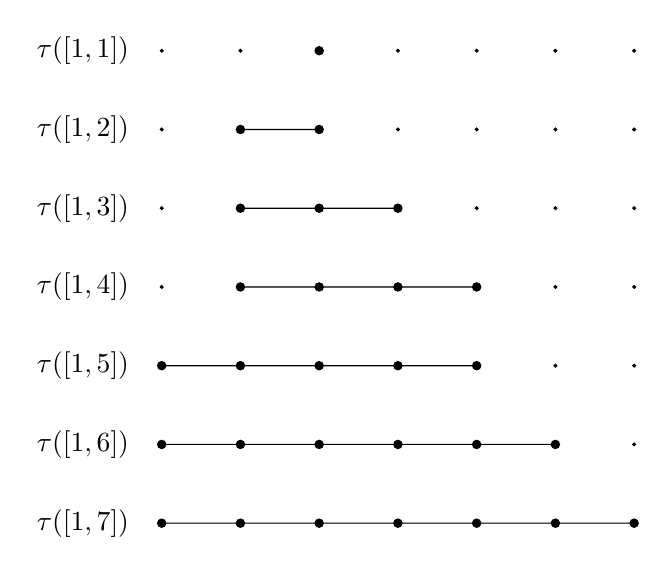
\begin{tikzpicture}
		\tikzset{
			c/.style={insert path={circle[radius=0.5pt]}},
			d/.style={insert path={circle[radius=1.5pt]}},
		}
		\draw[fill] (0,0)[c]  (1,0) [c] (2,0) [d] (3,0) [c] (4,0) [c] (5,0) [c] (6,0) [c];
		\draw[fill] (0,-1)[c] (1,-1) [d] -- (2,-1) [d] (3,-1) [c] (4,-1) [c] (5,-1) [c] (6,-1) [c];
		\draw[fill] (0,-2)[c] (1,-2) [d] -- (2,-2) [d]  -- (3,-2) [d] (4,-2) [c] (5,-2) [c] (6,-2) [c];
		\draw[fill] (0,-3)[c] (1,-3) [d] -- (2,-3) [d]  -- (3,-3) [d] -- (4,-3) [d] (5,-3) [c] (6,-3) [c];
		\draw[fill] (0,-4)[d] -- (1,-4) [d] -- (2,-4) [d]  -- (3,-4) [d] -- (4,-4) [d] (5,-4) [c] (6,-4) [c];
		\draw[fill] (0,-5)[d] -- (1,-5) [d] -- (2,-5) [d]  -- (3,-5) [d] -- (4,-5) [d] -- (5,-5) [d] (6,-5) [c];
		\draw[fill] (0,-6)[d] -- (1,-6) [d] -- (2,-6) [d]  -- (3,-6) [d] -- (4,-6) [d] -- (5,-6) [d] -- (6,-6) [d];
		\node (t1) at (-1,0) {$\tau([1,1])$};
		\node (t2) at (-1,-1) {$\tau([1,2])$};
		\node (t3) at (-1,-2) {$\tau([1,3])$};
		\node (t4) at (-1,-3) {$\tau([1,4])$};
		\node (t5) at (-1,-4) {$\tau([1,5])$};
		\node (t6) at (-1,-5) {$\tau([1,6])$};
		\node (t7) at (-1,-6) {$\tau([1,7])$};
	\end{tikzpicture}
	\caption{The elements of $\Xi_N$ are built by iteratively appending to the left or the right. Shown is a visual representation of the element $[3,2,4,5,1,6,7] \in \Xi_7$.}
	\label{fig:mental_picture_Xi_N}
\end{figure}

\begin{example}

	We show that the algebra $\Heis(\mcU_q(\mfn_2))$ from \cref{exmp:heisenberg} is a
	symmetric CGL extension. The first condition is verified easily by using
	\cref{table:sigma_delta_heisenberg}. For example, for $k = 5$ we have
	\begin{align*}
		 & \delta_5(x_1) = \delta_5(E_2) = (q\inv - q)F_1 \in R_{[2,4]},                   \\
		 & \delta_5(x_2) = \delta_5(E_{12}) = (q\inv - q)(F_1E_1 - E_1 F_1) \in R_{[3,4]}, \\
		 & \delta_5(x_3) = \delta_5(E_{1}) = 0 \in R_{[4,4]},                              \\
		 & \delta_5(x_3) = \delta_5(F_{1}) = 0 \in R_{[5,4]} = \bbK.
	\end{align*}
	%
	For the second condition, we can take
	\begin{align*}
		h_1^* & = h_1\inv =(1, q, q\inv), \quad h_4^* = h_4\inv = (q\inv, q, 1), \\
		h_2^* & = h_2\inv =(q, 1, q\inv), \quad h_5^* = h_5\inv = (q\inv,1, q),  \\
		h_3^* & = h_3\inv =(q, q\inv, 1), \quad h_6^* = h_6\inv = (1, q\inv, q).
	\end{align*}
	%
	Furthermore, $\lambda_1^* = \lambda_2^* = \cdots = \lambda_6^* = q^2$ is not a root of
	unity.
\end{example}

\textbf{Homogeneous prime elements.}

A \emph{prime element}\index{element!prime} of a not necessarily commutative domain $R$
is a nonzero element $p \in R$ such that $p$ is \emph{normal}\index{element!normal},
that is, $Rp = pR$ and such that the quotient $R / Rp$ is a domain. To illustrate that
this definition corresponds to our intuition of what a prime element should be, we
prove the following small lemma.
\begin{lemma}\label{lem:prime_divides_product}
	%
	Let $p$ be a prime element in a ring $R$. If $p$ divides a product $ab$ for some $a,b
		\in R$, then $p$ divides $a$ or $p$ divides $b$.
\end{lemma}
\begin{proof}
	%
	Note that since $p$ is normal, there is no ambiguity about dividing $ab$ on the left or
	on the right. Indeed, if $c p = ab$ for some $c \in R$, then $ab \in Rp = pR$, and
	there exists some $c' \in R$ such that $p c' = ab$. So, assume that $ab \in Rp$. Then
	the image of $ab$ is zero under the quotient map $\pi \colon R \to R/Rp$. Since $Rp$ is
	a domain, that implies that either $\pi(a) = 0$ or $\pi(b)$ is zero. So, either $a \in
		Rp$ or $b \in Rp$.
\end{proof}
%
We now state a theorem that is quite technical, but forms the heart of the main
theorem. Let us first fix some notation. For a function $\eta \colon [1, N] \to \bbZ$,
we can define a predecessor and successor
function\index{function!predecessor}\index{function!successor}:
\begin{align*}
	p \colon [1, N] \to [1, N] \sqcup \{-\infty\} & \colon k \mapsto  \max\{j < k \mid \eta(j) = \eta(k)\}  \\
	s \colon [1, N] \to [1, N] \sqcup \{+\infty\} & \colon k \mapsto  \min\{j > k \mid \eta(j) = \eta(k)\},
\end{align*}
%
where we take $\max \{\} = - \infty$ and $\min \{\}= + \infty$ (cf.
\cref{fig:predecessor_successor}).

\begin{figure}
	\centering
	\begin{tikzpicture}
		\draw[help lines, xstep =0] (0,0) grid (8,3);
		\draw plot[mark=*] coordinates {(1,1) (2,2) (3,1) (4,0) (5,1) (6,3) (7,2)};
		\node (neginf) at (-0.5,1) {$-\infty$};
		\node (a) at (1,1) {};
		\node (b) at (3,1) {};
		\node (c) at (5,1) {};
		\node (posinf) at (8.5, 1) {$+\infty$};
		\draw[Stealth-, red] (neginf) to [bend right = 20] (a);
		\draw[Stealth-Stealth, red] (a) to [bend right = 20] (b);
		\draw[Stealth-Stealth, red] (b) to [bend right = 20] (c);
		\draw[-Stealth, red] (c) to [bend right = 15] (posinf);
	\end{tikzpicture}
	\caption{The predecessor and successor functions move along the level sets (the horizontal lines) to the previous or the next point respectively.}
	\label{fig:predecessor_successor}
\end{figure}

\begin{theorem}[\protect{\cite[Theorem 3.6]{GoodearlYakimov2017QCA}}]\label{thm:homogeneous_primes}
	Let $R$ be a CGL extension of length $N$. There exists a function $\eta \colon [1, N] \to \bbZ$ and elements
	\begin{equation*}
		c_k \in R_{k-1} \text{ for all } k \in [2,N] \text{ with } p(k) \neq - \infty
	\end{equation*}
	such that the elements $y_1, \dots, y_N \in R$, recursively defined by
	\begin{equation*}
		y_k = \begin{cases}
			y_{p(k)}x_k - c_k & \text{ if } p(k) \neq -\infty \\
			x_k               & \text{ if } p(k) = -\infty,
		\end{cases}
	\end{equation*}
	%
	are homogeneous and have the property that for every $k \in [1, N]$,
	\begin{equation}\label{eq:list_of_ys_in_R_k}
		\{y_j \mid j \in [1, k], s(j) > k\}
	\end{equation}
	%
	is a list of the homogeneous prime elements of $R_k$, up to scalar multiples. The
	elements $y_1, \dots, y_N \in R$ with these properties are unique, and the function $p$
	has the property that $p(k) = - \infty$ if and only if $\delta_k = 0$.
\end{theorem}

To compute the elements $y_1, \dots, y_N$, some additional facts come in handy. For
this, we introduce some further notation and relations related to CGL extensions. In
what follows, $R$ is a CGL extension and the elements $y_k, k \in [1, N]$ and the
functions $p$ and $s$ are as in \cref{thm:homogeneous_primes}.

Let $O_{\pm} \colon [1, N] \to \bbZ_{\geq 0}$ be the order
functions\index{function!order} given by
\begin{align*}
	O_{+}(k) & = \max\{m \in \bbZ_{\geq 0} \mid s^m(k) \neq + \infty\}   \\
	O_{-}(k) & = \max\{m \in \bbZ_{\geq 0} \mid p^m(k) \neq - \infty\} ,
\end{align*}
%
where we take $p^0 = s^0 = \id$. Define
\begin{equation*}
	\overline{e}_k = \sum_{m=0}^{O_{-}(k)} e_{p^m(k)} \in \bbZ^N,
\end{equation*}
%
for $k \in [1, N]$. Then, for $j,k \in [1, N]$, set
\begin{equation*}
	\alpha_{kj} = \Omega_{\bbl}(e_k, \overline{e}_j) = \prod_{m=0}^{O_{-}(j)}\lambda_{k, p^m(j)} \in \bbK^\times
\end{equation*}
and
\begin{equation*}
	q_{kj} = \Omega_{\bbl}(\overline{e}_k, \overline{e}_j) = \prod_{m=0}^{O_{-}(k)}\prod_{l=0}^{O_{-}(j)}\lambda_{p^m(k),p^l(j)} = \prod_{m=0}^{O_{-}(k)}\alpha_{p^m (k),j} \in \bbK^\times,
\end{equation*}
%
where $\bbl$ is as defined in \cref{eq:CGL_lambda}. Write $\bmq = (q_{kj}) \in
	M_N(\bbK^\times)$.
\begin{proposition}[\protect{\cite[Proposition 3.11]{GoodearlYakimov2017QCA}}]\label{prop:y_quantum_torus}
	The $y_k$ quasi-commute:
	\begin{equation}\label{eq:y_quasi_commute}
		y_k y_j = q_{kj}y_jy_k, \quad \forall j, k \in [1, N].
	\end{equation}
	%
	The quantum torus $\mcT_{\bmq}$ embeds in $\Fract(R)$ via the $\bbK$-algebra
	homomorphism $\varphi \colon \mcT_{\bmq} \injto \Fract(R)$ given by $\varphi(Y_i) =
		y_i,\,\forall i \in [1, N]$, and this embedding gives rise to inclusions
	\begin{equation*}
		\varphi(\mcA_{\bmq}) \subseteq R \subset \varphi(\mcT_{\bmq}) \subset \Fract(R).
	\end{equation*}
\end{proposition}

Additionally, we have the following equations.
\begin{align}\label{eq:y_x_quasi_commute}
	y_j x_k            & = \alpha_{kj}\inv x_k y_j, \text{ for all } j, k \in [1, N] \text{ such that } s(j) > k                                             \\
	\sigma_k (y_j)     & = \alpha_{kj}y_j, \text{ for } 1 \leq j \leq k \leq N \label{eq:sigma_of_y}                                                         \\
	\delta_k(y_{p(k)}) & = \alpha_{k, p(k)}(\lambda_k - 1)c_k, \text{ for all } k \in [2, N] \text{ such that } p(k) \neq - \infty \label{eq:delta_of_y_pk}.
\end{align}
%
From this we can deduce a small lemma that is useful for finding the sequence of
homogeneous prime elements $y_1, \dots, y_N$ of \cref{thm:homogeneous_primes}.
\begin{lemma}\label{lem:delta_nonzero_iff_predecessor}
	For all $1 \leq j < k \leq N$ such that $p(k) \neq -\infty$ and $s(j) \geq k$, we have $\delta_k(y_j) \neq 0$ if and only $s(j) = k$.
\end{lemma}
\begin{proof}
	First, suppose that $s(j) = k$. Then $p(k) = j$, and \cref{eq:delta_of_y_pk} gives that $\delta_k(y_j)$ is a scalar multiple of $c_k$, which is nonzero. Indeed, $c_k \neq 0$ because $p(k) \neq -\infty$ and $\lambda_k \neq 1$ because it is not a root of unity. Now, suppose that $s(j) > k$. Then \cref{eq:y_x_quasi_commute,eq:sigma_of_y} give that
	\begin{equation*}
		\alpha_{kj}y_jx_k = x_k y_j = \sigma_k(y_j) x_k + \delta_k(y_j) = \alpha_{kj}y_j x_k + \delta_k(y_j),
	\end{equation*}
	so that we must have $\delta_k(y_j) = 0$.
\end{proof}

% Finally, the following proposition provides a semi-constructive way of computing the
% $y_k$.
% \begin{proposition}[\protect{\cite[Proposition 3.10]{GoodearlYakimov2017QCA}}]\label{prop:constructive_hom_primes}
% 	Assume that $y_1', \dots, y_N'$ and $c_1',\dots, c_N'$ are two sequences of elements of $R$ such that
% 	\begin{enumerate}
% 		\item $y_1', \dots, y_N'$ are homogeneous normal elements of $R_1, \dots, R_N$ respectively.
% 		\item $c'_k \in R_{k-1}, \forall k \in [1, N]$.
% 		\item For every $k \in [1, N]$, if $\delta_k = 0$ then $y'_k = x_k$ and otherwise there
% 		      exists $j \in [1, k-1]$ such that $y'_k = y'_j x_k - c'_k$.
% 	\end{enumerate}
% 	Then $y_1' = y_1, y_2' = y_2, \dots, y_N' = y_N$.
% \end{proposition}

% With these preparations, we can now work out the homogeneous prime elements of \cref{thm:homogeneous_primes} for \cref{exmp:heisenberg}.

\begin{example}
	The goal is to find the sequence $y_1, y_2, \dots, y_6$ of homogeneous prime elements from \cref{thm:homogeneous_primes} for $R = \HeisUqn$. To do this, we make use of \cref{lem:delta_nonzero_iff_predecessor}.

	Since $\delta_1 = 0$ and $\delta_2 = 0$ we must have $y_1 = x_1 = E_2$ and $y_2 = x_2 =
		E_{12}$. Let $\eta \colon [1, 6] \to \bbZ$ denote the function from
	\cref{thm:homogeneous_primes}, and $p,s$ the corresponding predecessor and successor
	functions. Since $p(1) = p(2) = -\infty$ we must have $\eta(1) \neq \eta(2)$. Let us
	take $\eta(1) = 1$ and $\eta(2) = 2$.

	Because $\delta_3 \neq 0$, we know that $y_3$ is of the form $y_j x_3 - c_3 = y_j E_1 -
		c_3$ for some $j \in [1,2]$ and $c_3 \in R_{2}$. Since
	\begin{align*}
		\delta_3(y_2) = \delta_3(E_{12}) = 0,
	\end{align*}
	%
	we find, using \cref{lem:delta_nonzero_iff_predecessor}, that $p(3) \neq 1$. Thus, we
	must have $\eta(3) = 1$ and $j = p(3) = 1$. In this case,
	\begin{equation*}
		\delta_3(y_{p(3)}) = \delta_3(y_1) = \delta_3(E_2) = q E_{12}.
	\end{equation*}
	%
	Thus, from \cref{eq:delta_of_y_pk,eq:heisenberg_lambda_k}, we obtain
	\begin{equation*}
		c_3 = \alpha_{3,1}\inv (\lambda_3-1)\inv \delta_3(E_2) = q\inv \frac{1}{q^{-2}-1}(-q E_{12}) = \frac{1}{1 - q^{-2}}E_{12},
	\end{equation*}
	and hence
	\begin{equation*}
		y_3 = E_2 E_1 - \frac{1}{1-q^{-2}}E_{12} = \frac{1}{1-q^2}(E_2 E_1 - q E_1 E_2).
	\end{equation*}

	Again, since $\delta_4 \neq 0$, we know that $y_4 = y_j F_1 -c_4$ for some $j \in [1,
			3]$ and $c_4 \in R_3$. Furthermore, we know that $j = p(4)$. So, since $\eta(1) =
		\eta(3)$, we must have $j = 2$ or $j = 3$. The case $j = 2$ can be ruled out because,
	$\delta_4(y_2) = \delta_4(E_{12}) = 0$. Thus, $\eta(4) = 1$ and $j = p(4) = 3$. We can
	now compute $c_4$ using \cref{eq:delta_of_y_pk}. We have, using
	\cref{table:sigma_delta_heisenberg},
	\begin{align*}
		\delta_4(y_{p(4)})
		 & = \delta_4(y_3)                                                                                                                \\
		 & = \delta_4\Bigl(\frac{1}{1-q^2}(E_2 E_1 - q E_1 E_2)\Bigr)                                                                     \\
		 & = \frac{1}{1-q^2}\Bigl(\sigma_4 (E_2)\delta_4(E_1) + \delta_4(E_2)E_1 - q(\sigma_4(E_1)\delta_4(E_2) + \delta_4(E_1)E_2)\Bigr) \\
		 & = \frac{1}{1-q^2}\Bigl(q\inv E_2  - qE_2\Bigr)                                                                                 \\
		 & = \frac{1}{1-q^2} q\inv (1- q^2) E_2                                                                                           \\
		 & = q\inv E_2.
	\end{align*}
	%
	Hence, from \cref{table:sigma_delta_heisenberg,eq:heisenberg_lambda_k}, we obtain
	\begin{align*}
		c_4 & = \alpha_{4,3}\inv (\lambda_4 - 1)\inv \delta_4(y_3)           \\
		    & = \lambda_{4,3}\inv\lambda_{4,1}\inv (q^{-2} -1)\inv q\inv E_2 \\
		    & = \frac{q^{-2}qq\inv}{q^{-2} - 1} E_2                          \\
		    & = \frac{1}{1 - q^2} E_2,
	\end{align*}
	and consequently
	\begin{equation*}
		y_4 = y_3 F_1 - \frac{1}{1-q^2}E_2.
	\end{equation*}

	For $y_5$ we must have either $p(5) = 2$ or $p(5) = 4$. Let us first assume that $p(5)
		= 4$. Then we would have
	\begin{align*}
		\delta_5(y_{p(5)})
		 & = \delta_5(y_4)                                                                                 \\
		 & = \delta_5\Bigl(y_3F_1 - \frac{1}{1-q^2}\delta_5(E_2)\Bigr)                                     \\
		 & = \delta_5(y_3)F_1 - \frac{1}{1-q^2}(q\inv -q) F_1                                              \\
		 & = \frac{1}{1-q^2}\Bigl(\delta_5(E_2)E_1 - q \sigma_5 (E_1) \delta_5(E_2) - (q\inv -q)\Bigr) F_1 \\
		 & = \frac{q\inv - q}{1-q^2}\bigl(F_1E_1 - q^2 E_1 F_1 - 1\bigr) F_1                               \\
		 & = 0.
	\end{align*}
	%
	Thus \cref{eq:delta_of_y_pk} gives $c_5 = 0$, a contradiction. So, $p(5) = 2$ and
	$\eta(5) = \eta(2)$. We find
	\begin{align*}
		\delta_5(y_{p(5)})
		 & = \delta_5(y_2)                                                          \\
		 & = \delta_5(E_{12})                                                       \\
		 & = (q\inv -q)(F_1E_1 - E_1F_1)                                            \\
		 & = (q\inv -q)(1 + (q^2 - 1)E_1 F_1),
		\intertext{and hence}
		c_5
		 & = \alpha_{5, 2}\inv (\lambda_5 - 1)\inv \delta_5(y_{p(5)})               \\
		 & = \lambda_{5, 2}\inv (q^{-2} - 1)\inv (q\inv - q)(1 + (q^2 - 1) E_1 F_1) \\
		 & = q^{-2} (q^{-2} - 1)\inv q (q^{-2} - 1)(1 + (q^2 - 1) E_1 F_1)          \\
		 & = q\inv + (q - q\inv) E_1 F_1.
	\end{align*}
	%
	We have thus shown that
	\begin{align*}
		y_5 = y_2 F_{12} + (q\inv - q) E_1 F_1 - q\inv.
	\end{align*}
	%
	Note that if we would have first calculated $\delta_5(y_2)$, then we could have avoided
	calculating $\delta_5(y_4)$, since we would already know that it is zero by
	\cref{lem:delta_nonzero_iff_predecessor}.

	We now move on to calculating the final homogeneous prime element, $y_6$. There are two
	possibilities, $p(6) = 4$ or $p(6) = 5$. We first determine $\delta_6(y_4)$:
	\begin{align*}
		\delta_6(y_4)
		 & = \delta_6\bigl(y_3F_1- \frac{1}{1-q^2}E_2\bigr)                                        \\
		 & = \delta_6\bigl(y_3F_1- \frac{1}{1-q^2}E_2\bigr)                                        \\
		 & = \sigma_6(y_3)F_{12} + \frac{1}{1-q^2}\delta_6(E_2E_1 - q E_1 E_2)F_1- \frac{1}{1-q^2} \\
		 & = qy_3F_{12} + \frac{1}{1-q^2}(E_1 - E_1)F_1- \frac{1}{1-q^2}                           \\
		 & = qy_3F_{12} - \frac{1}{1-q^2}.
	\end{align*}
	%
	Since it is nonzero, we conclude using \cref{lem:delta_nonzero_iff_predecessor} that
	$p(6) = 4$ and $\delta_6(y_5) = 0$. Hence,
	\begin{align*}
		c_6
		 & = \alpha_{6, 4}\inv (q^{-2} - 1)\inv \delta_6(y_4)                                                             \\
		 & = (\lambda_{6,4}\lambda_{6,3}\lambda_{6,1})\inv \frac{1}{q^{-2} - 1}\Bigl(q y_3 F_{12} - \frac{1}{1-q^2}\Bigr) \\
		 & = \frac{1}{1 -q^{2}}\Bigl(q y_3 F_{12} - \frac{1}{1-q^2}\Bigr),
	\end{align*}
	and
	\begin{equation*}
		y_6 = y_4 F_2 - \frac{1}{1-q^2}\Bigl(q y_3 F_{12} + \frac{1}{1-q^2}\Bigr).
	\end{equation*}

	We now briefly summarize all the findings. The $\eta$-function of
	\cref{thm:homogeneous_primes} for the algebra $\HeisUqn$ can be taken to be $\eta
		\colon [1, 6] \to \bbZ$ with $\eta(1)=\eta(3)=\eta(4)=\eta(6) = 1$ and $\eta(2) =
		\eta(5) = 2$. The sequence of homogeneous prime elements is given by
	\begin{align*}
		y_1 & = E_2                                                                      \\
		y_2 & = E_{12}                                                                   \\
		y_3 & = y_1 E_1 - \frac{1}{1- q^{-2}}E_{12}                                      \\
		y_4 & = y_3 F_1 - \frac{1}{1-q^2} E_2                                            \\
		y_5 & = y_2 F_{12} - (q - q\inv) E_1 F_1 - q \inv                                \\
		y_6 & = y_4 F_2 - \frac{1}{1-q^2} \Bigl(q y_3 F_{12} - \frac{1}{1 - q^2} \Bigr).
	\end{align*}
	%
	To visualize $\eta$ as well as the predecessor and successor functions, we can think of
	them arranged as follows:
	\begin{equation*}
		\begin{tikzcd}[sep=tiny]
			& y_2 & & & y_5 \\
			y_1 & & y_3 & y_4 & & y_6
		\end{tikzcd}
	\end{equation*}

\end{example}

\subsection{The main theorem}

To obtain a cluster algebra structure on a symmetric CGL extension, we need to study
how the homogeneous prime elements change when the variables $x_1, \dots, x_N$ are
adjoined in a different order. We consider the most basic case, when we swap the order
of two adjacent variables $x_k, x_{k+1}$. So, we have a CGL extension
\begin{equation}\label{eq:default_cgl_presentation}
	R = \bbK[x_1][x_2; \sigma_2, \delta_2]\cdots[x_k; \sigma_k, \delta_k][x_{k+1};\sigma_{k+1}, \delta_{k+1}]\cdots[x_N; \sigma_N, \delta_N],
\end{equation}
%
such that we can also write $R$ as a CGL extension of the form
\begin{multline}\label{eq:swapped_cgl_presentation}
	R = \bbK[x_1][x_2; \sigma_2, \delta_2]\cdots[x_{k-1}; \sigma_{k-1}, \delta_{k-1}][x_{k+1}; \sigma_k', \delta_k'][x_k;\sigma_{k+1}', \delta_{k+1}']\\
	[x_{k+2}; \sigma_{k+2}, \delta_{k+2}]\cdots[x_N; \sigma_N, \delta_N].
\end{multline}
%
We will denote the chain of algebras as
\begin{equation*}
	\bbK = R'_0 \subset R'_1  = \bbK[x_1] \subset R'_2 = \bbK[x_1][x_2; \sigma_2, \delta_2] \subset \cdots \subset R'_N = R
\end{equation*}
for the presentation \eqref{eq:swapped_cgl_presentation}.
We first look at what restrictions this places on the $\sigma_i, \sigma_i '$ and
$\delta_i,\delta_i'$ appearing in the CGL presentations.
\begin{lemma}\label{lem:swapped_cgl_sigma_delta}
	Let $R$ be a CGL extension with presentations of the form \eqref{eq:default_cgl_presentation} and \eqref{eq:swapped_cgl_presentation}. Then
	\begin{equation}\label{eq:sigma_prime}
		\begin{aligned}
			\sigma_k ' & = \sigma_{k+1}|_{R_{k-1}}    \\
			\sigma_k   & = \sigma_{k+1}' |_{R_{k-1}},
		\end{aligned}
	\end{equation}
	and
	\begin{equation}\label{eq:delta_prime}
		\begin{aligned}
			\delta_k ' & = \delta_{k+1}|_{R_{k-1}}    \\
			\delta_k   & = \delta_{k+1}' |_{R_{k-1}}.
		\end{aligned}
	\end{equation}
	Furthermore, $\delta_{k+1}(x_k) \in R_{k-1}$ and
	\begin{equation}\label{eq:sigma_delta_prime_x_k_1}
		\begin{aligned}
			\sigma_{k+1}'(x_{k+1}) & = \lambda_{k, k+1} x_{k+1}             \\
			\delta_{k+1}'(x_{k+1}) & = -\lambda_{k, k+1} \delta_{k+1}(x_k).
		\end{aligned}
	\end{equation}
	%
\end{lemma}
\begin{proof}
	%
	From \cref{eq:default_cgl_presentation} we have that $x_{k+1}a = \sigma_{k+1}(a)x_{k+1}
		+ \delta_{k+1}(a)$ for $a \in R_{k-1}$. On the other hand, also $x_{k+1}a =
		\sigma_k'(a)x_{k+1} + \delta_k'(a)$ using \cref{eq:swapped_cgl_presentation}. So
	\begin{equation*}
		\sigma_{k+1}(a)x_{k+1} + \delta_{k+1}(a) = \sigma_k'(a) x_{k+1} + \delta_k'(a).
	\end{equation*}
	%
	Using that $\sigma_k'(a)\in R_{k-1}, \sigma_{k+1}(a) \in R_k$ and $\delta_k'(a) \in
		R_{k-1}, \delta_{k+1}(a) \in R_{k}$ together with the fact that $x_{k+1}$ and 1 are
	linearly independent over $R_k$ it follows that $\sigma_k'(a) = \sigma_{k+1}(a)$ and
	$\delta_k'(a) = \delta_{k+1}(a)$. Applying the same reasoning, but swapping the roles
	of \cref{eq:default_cgl_presentation,eq:swapped_cgl_presentation} we obtain
	$\sigma_k(a) = \sigma_{k+1}'(a)$ and $\delta_k(a) = \delta_{k+1}'(a)$, and we have
	shown \cref{eq:delta_prime,eq:sigma_prime}.

	Recalling \cref{eq:CGL_lambda}, note that $x_k x_{k+1} = \lambda'_{k+1,k}x_{k+1}x_{k} +
		\delta'_{k+1}(x_{k+1})$, and $\lambda'_{k,k+1} = (\lambda_{k+1, k}')\inv$. So,
	\begin{equation*}
		\lambda'_{k,k+1}x_k x_{k+1} - \lambda'_{k,k+1} \delta'_{k+1}(x_{k+1}) = x_{k+1} x_k = \lambda_{k+1, k} x_k x_{k+1} + \delta_{k+1}(x_k).
	\end{equation*}
	%
	Then, since $\delta'_{k+1} \in R'_k $ and $\delta_{k+1}(x_k) \in R_k$ are linearly
	independent of $x_k x_{k+1}$ over $R_{k-1}$, we must have $\lambda_{k,k+1}' =
		\lambda_{k+1,k}$ and
	\begin{equation*}
		-\lambda'_{k,k+1}\delta'_{k+1}(x_{k+1}) = \delta_{k+1}(x_k) \in R'_k \cap R_k = R_{k-1}.
	\end{equation*}
	%
	Thus,
	\begin{align*}
		\sigma'_{k+1}(x_{k+1}) & = \lambda'_{k+1,k}x_{k+1} = \lambda_{k, k+1}x_{k+1}         \\
		\delta'_{k+1}(x_{k+1}) & = -(\lambda_{k,k+1}')\inv \delta_{k+1}(x_k) = - \lambda_{k,
			k+1}\delta_{k+1}(x_k),
	\end{align*}
	showing \cref{eq:sigma_delta_prime_x_k_1}.
\end{proof}

Using the previous lemma, we can now describe what happens to the homogeneous prime
elements $y_1, \dots, y_N$.

\begin{theorem}\label{thm:y_prime_swapped_cgl}
	Assume that $R$ is a CGL extension of the form \eqref{eq:default_cgl_presentation}, with a second CGL presentation of the form \eqref{eq:swapped_cgl_presentation}. Denote with $y_1, \dots, y_N$ the sequence of homogeneous prime elements from \cref{thm:homogeneous_primes}, and $\eta : [1, N] \to \bbZ$ the associated function for \eqref{eq:default_cgl_presentation}. For \eqref{eq:swapped_cgl_presentation} we write $y'_1, \dots, y'_N$ and $\eta'$.
	\begin{enumerate}[(a)]
		\item If $\eta(k) \neq \eta(k+1)$, then $y'_j = y_j$ for $j \neq k, k+1$ and $y'_k = y_{k+1},
			      y'_{k+1} = y_k$.

		\item \label{itm:eta_k_is_eta_k_plus_one} If $\eta(k) = \eta(k+1)$,
		      then
		      \begin{equation*}
			      y_k y'_k - \alpha_{k p(k)} y_{p(k)} y_{k+1}
		      \end{equation*}
		      is a homogeneous normal element of $R_{k-1}$, where we take $y_{-\infty} = 1 =
			      \alpha_{k, -\infty}$. From \cref{eq:y_x_quasi_commute} we know that $y_{p(k)}y_{k+1}
			      x_j = \gamma_j y_{p(k)}y_{k+1}$ for some $\gamma_j \in \bbK$ for each $j \in [1, k-1]$.
		      Then, also
		      \begin{equation*}
			      (y_ky'_k - \alpha_{kp(k)}y_{p(k)}y_{k+1})x_j = \gamma_j x_j (y_ky'_k - \alpha_{kp(k)}y_{p(k)}y_{k+1}).
		      \end{equation*}
		      Moreover,
		      \begin{equation}\label{eq:y_prime_in_swapped_cgl}
			      y'_j = \begin{dcases*}
				      \lambda_{k+1,k}y_j, & if $j=s^l(k+1)$ for some $l \in \bbZ_{\geq 0}$                               \\
				      y_j,                & if $j < k$, or $j>k+1$ and $j \neq s^l (k+1)$ for all $l \in \bbZ_{\geq 0}$.
			      \end{dcases*}
		      \end{equation}
	\end{enumerate}
	In both cases, we can take $\eta' = \eta \circ (k,k+1)$, where $(k, k+1)$ denotes a transposition in $S_N$.
\end{theorem}
\begin{proof}
	%
	Since $R'_j = R_j$ for $j\neq k, k+1$ we also have that $y'_j = y_j$ for $j\in [1,
			k-1]$ since they only depend recursively on the ones before. We can hence also choose
	$\eta'(j) = \eta(j)$ for all $j\in [1, k-1]$. As we already remarked in the previous
	lemma, $R'_k \cap R_k = R_{k-1}$, and hence $y'_k$ which lies in $R'_k$ but not in
	$R_{k-1}$ is not contained in $R_k$.

	If $\eta(k) \neq \eta(k+1)$, then $s(k) > k+1$, and hence $y_k$ is a homogeneous prime
	element of $R_{k+1}$ due to \cref{eq:list_of_ys_in_R_k}. So, $R_{k+1}$ has two
	homogeneous prime elements up to taking scalar multiples, $y_k$ and $y_{k+1}$, which do
	not belong to $R_{k-1}$. Since $R_{k-1}' = R_{k-1}$ and $R_{k+1}' = R_{k+1}$, it
	follows that $\eta'(k) \neq \eta'(k+1)$. Indeed, $s'(k) = k+1$ would mean that $y'_k$
	is not a homogeneous prime element of $R'_{k+1}$, and $R'_{k+1}$ would only have one
	homogeneous prime element up to taking associates which doesn't belong to $R_{k-1}$.
	Now, by the uniqueness up to taking associates of the homogeneous prime elements and
	the fact that $y'_k \notin R_k$, we have that $y'_k = \xi_{k+1}y_{k+1}$ and $y'_{k+1} =
		\xi_{k}y_k$ for some $\xi_k, \xi_{k+1} \in \bbK^\times$. Since $y_j' = y_j$ for $j \in
		[1, k-1]$, \cref{thm:homogeneous_primes} gives that $\xi_{k} = 1 \xi_{k+1}$, and that
	we may choose $\eta'(k) = \eta(k+1)$ and $\eta'(k+1) = \eta(k)$. Additionally, since
	$R'_j = R_j$ for $j \in [k+1, N]$, we have $y'_j = \xi_j y_j$ for some $\xi_j \in
		\bbK^\times$. Applying \cref{thm:homogeneous_primes} and looking at the leading
	coefficients, we find that $\xi_j = 1$ and that we may choose $\eta'(j) = \eta(j)$ for
	all $j \in [k+1, N]$. \medskip

	If $\eta(k) = \eta(k+1)$, then $s(k) = k+1$ so that $y_k$ is not a homogeneous prime
	element of $R_{k+1}$. So, $y_{k+1}$ is the only homogeneous prime element, up to taking
	associates, in $R_{k+1}\setminus R_{k-1}$. Since $R'_{k+1} = R_{k+1}$ and $R'_{k-1} =
		R_{k-1}$ we must have that $y'_{k+1}$ is a scalar multiple of $y_{k+1}$, and that
	$\eta'(k) = \eta'(k+1)$. Because $\eta'(k) = \eta'(p(k)) = \eta(p(k))$ if $p(k) \neq
		-\infty$, we may choose $\eta'(k) = \eta'(k+1) = \eta(k+1) = \eta(k)$. Using this
	information, \cref{thm:homogeneous_primes} gives
	\begin{equation}\label{eq:recursive_yk_y_k_prime}
		\begin{alignedat}{2}
			y_k &= \begin{dcases*}
				\mathrlap{y_{p(k)}x_k - c_k,}\hphantom{y_{p(k)}x_{k+1}-c'_k,} & if $p(k) \neq -\infty$ \\
				x_k,                                                          & if $p(k) = -\infty$
			\end{dcases*}
			&
			y_{k+1} &= y_k x_{k+1} - c_{k+1}\\
			y'_k    & = \begin{dcases*}
				y_{p(k)}x_{k+1} - c'_k, & if $p(k) \neq -\infty$ \\
				x_{k+1},                & if $p(k) = -\infty$
			\end{dcases*}
			\qquad
			&
			y_{k+1} & = y'_k x_k - c'_{k+1}
		\end{alignedat}
	\end{equation}
	%
	for some $c_k,c'_k \in R_{k-1}, c_{k+1} \in R_k$ and $c'_{k+1} \in R'_{k}$. Now,
	\begin{align*}
		y_{k+1}  & = y_k x_{k+1} - c_{k+1} = y_{p(k)} x_k x_{k+1} - c_{k+1} - c_k x_{k+1} ,                                                        \\
		\shortintertext{and}
		y'_{k+1} & = y'_k x_k - c'_{k+1} = y_{p(k)}x_{k+1}x_k - c'_{k+1} - c'_k x_k = \lambda_{k+1, k}y_{p(k)}x_k x_{k+1} - c'_{k+1} - c'_{k} x_k,
	\end{align*}
	%
	where we use the convention that $y_{p(k)} = 1$ and $c'_k = c_k = 0$ if $p(k) =
		-\infty$. Since $y'_{k+1}$ is a scalar multiple of $y_{k+1}$, we must have
	\begin{equation*}
		y'_{k+1} = \lambda_{k+1,k}y_{k+1}.
	\end{equation*}
	%
	Using again that $R'_j = R_j$ for $j \in [k+1, N]$, together with
	\cref{thm:homogeneous_primes} we find $\eta'(j) = \eta(j)$ for $j\in [k+1, N]$ and
	$y'_j = \lambda_{k+1,k} y_j$ if $j = s^l(k+1)$ for some $l \in \bbZ_{\geq 0}$ while
	$y'_j = y_j$ otherwise.

	We now verify that
	\begin{equation*}
		y_k y'_k - \alpha_{k p(k)}y_{p(k)}y_{k+1} \in R_{k-1}.
	\end{equation*}
	%
	If $p(k) = -\infty$, then $y_k = x_k$ and
	\begin{equation*}
		c_{k+1} \overset{\eqref{eq:delta_of_y_pk}}{=} \alpha_{k+1, p(k+1)}\inv (\lambda_{k+1} - 1)\inv\delta_{k+1}(y_{p(k+1)})
		= \alpha_{k+1, k}\inv (\lambda_{k+1} -1)\inv \delta_{k+1}(x_k) \in R_{k-1},
	\end{equation*}
	%
	as $\delta_{k+1}(x_k) \in R_{k-1}$ by \cref{lem:swapped_cgl_sigma_delta}. By
	convention, $y_{-\infty} = 1 = \alpha_{k, -\infty}$. Hence,
	\begin{equation}\label{eq:y_k_y_k_prime_when_pk_inf}
		y_k y'_k - \alpha_{kp(k)}y_{p(k)}y_{k+1} = y_k y'_k - y_{k+1} =  x_k x_{k+1} - (x_k x_{k+1} - c_{k+1}) = c_{k+1} \in R_{k-1},
	\end{equation}
	as desired, and we also immediately obtain that it is homogeneous, as $c_{k+1} = y_k x_{k+1} -y_{k+1}$ is homogeneous.

	Now, let us tackle the case where $p(k) \neq -\infty$. We have
	\begin{align*}
		y_k y_{p(k)}  \overset{\eqref{eq:recursive_yk_y_k_prime}} & {=} (y_{p(k)}x_k - c_k)y_{p(k)}                       \\
		\overset{\eqref{eq:y_x_quasi_commute}}                    & {=} y_{p(k)}\sigma_k(y_{p(k)}) x_k - c_k y_{p(k)}     \\
		\overset{\eqref{eq:sigma_of_y}}                           & {=} \alpha_{kp(k)} y_{p(k)}y_{p(k)}x_k - c_k y_{p(k)} \\
		\overset{\eqref{eq:y_quasi_commute}}                      & {=} \alpha_{kp(k)}y_{p(k)}y_k,
	\end{align*}
	and hence
	\begin{align*}
		y_k y'_k - \alpha_{kp(k)}y_{p(k)}y_{k+1} & = y_k (y_{p(k)}x_{k+1}-c'_k) -\alpha_{kp(k)}y_{p(k)}(y_kx_{k+1}-c_{k+1}) \\
		                                         & = -y_k c'_k + \alpha_{kp(k)}y_{p(k)}c_{k+1} \in R_k.
	\end{align*}
	%
	On the other hand,
	\begin{align*}
		\sigma'_{k+1}(y'_k)                          & = \sigma'_{k+1}(y_{p(k)}x_{x+1} - c'_k)                                \\
		\overset{\eqref{eq:sigma_delta_prime_x_k_1}} & {=} \alpha_{kp(k)}\lambda_{k,k+1}y_{p(k)}x_{k+1} - \sigma_{k+1}'(c'_k) \\
		\overset{\eqref{eq:sigma_of_y}}              & {=} \alpha_{kp(k)}\lambda_{k+1,k}\inv y'_k,
	\end{align*}
	from which we obtain
	\begin{align*}
		y_k y_k' - \alpha_{kp(k)}y_{p(k)}y_{k+1} & = (y_{p(k)}x_k -c_k)y'_k -\alpha_{kp(k)}y_{p(k)}\lambda_{k+1,k}\inv y_{p(k)} y'_{k+1}                                                       \\
		                                         & = y_{p(k)}(\sigma'_{k+1}(y'_k)x_k + \delta'_{k+1}(y'_k)) -c_k y'_k -\alpha_{kp(k)}y_{p(k)}\lambda_{k+1,k}\inv y_{p(k)}(y'_k x_{k}-c'_{k+1}) \\
		                                         & = y_{p(k)}\delta'_{k+1}(y'_k) -c_k y'_k -\alpha_{kp(k)}y_{p(k)}\lambda_{k+1,k}\inv y_{p(k)}c'_{k+1} \in R'_k.
	\end{align*}
	%
	So, $y_k y_k'- \alpha_{kp(k)}y_{p(k)}y_{k+1} \in R_k \cap R_k' = R_{k-1}$, which is
	what we wanted to show. Let us now show that it is also homogeneous in this case.

	By \cref{eq:delta_of_y_pk}, $c'_k$ and $c_{k+1}$ are scalar multiples of $\delta'_k
		(y_{p(k)}) = \delta_{k+1}(y_{p(k)})$ and $\delta_{k+1}(y_k)$ respectively. So, by
	\cref{lem:h_after_delta}, we have that
	\begin{align*}
		h \cdot (y_k c'_k)        & = \chi_{y_k}(h)y_k h \cdot (\xi \delta_{k+1}(y_{p(k)}))                              \\
		                          & = \chi_{y_k}(h)y_k \chi_{x_{k+1}}(h) \chi_{y_{p(k)}}(h)\xi \delta_{k+1}(y_{p(k)})    \\
		                          & = \chi_{y_k}(h)\chi_{x_{k+1}}(h)\chi_{y_{p(k)}}(h) y_k c'_k                          \\
		\shortintertext{and}
		h \cdot (y_{p(k)}c_{k+1}) & = \chi_{y_{p(k)}}(h) y_{p(k)} h \cdot (\xi' \delta_{k+1}(y_k))                       \\
		                          & = \chi_{y_{p(k)}}(h)y_{p(k)}  \chi_{x_{k+1}}(h) \chi_{y_k}(h) \xi' \delta_{k+1}(y_k) \\
		                          & = \chi_{y_{p(k)}}(h)  \chi_{x_{k+1}}(h) \chi_{y_k}(h) y_{p(k)}c_{k+1},
	\end{align*}
	%
	for all $h \in \mcH$. Hence, $-y_k c'_k + \alpha_{kp(k)}y_{p(k)}c_{k+1} = y_k y'_k -
		\alpha_{kp(k)}y_{p(k)}y_{k+1}$ is homogeneous.

	It remains to show that it is normal in $R_{k-1}$. By \cref{eq:y_x_quasi_commute}, we
	get that
	\begin{equation*}
		(y_k y_k')x_j = \beta_j x_j (y_k y'_k),
	\end{equation*}
	and
	\begin{equation*}
		(y_{p(k)}y_{k+1})x_j = \gamma_j x_j (y_{p(k)}y_{k+1}),
	\end{equation*}
	for all $j \in [1, k-1]$, where
	\begin{align*}
		\beta_j & = (\alpha'_{jk})\inv \alpha_{jk} \inv                                                                                   \\
		        & = \left(\prod_{m = 0}^{O_{-}(k)}\lambda_{j,p^m (k)} \prod_{l=0}^{O_{-}(k)}\lambda'_{j,p^l(k)}\right)\inv                \\
		        & = \left(\lambda_{j, k+1}\prod_{m = 0}^{O_{-}(k)}\lambda_{j,p^m (k)} \prod_{l=1}^{O_{-}(k)}\lambda_{j,p^l(k)}\right)\inv \\
		        & = \left(\prod_{m = 0}^{O_{-}(k+1)}\lambda_{j,p^m (k)} \prod_{l=0}^{O_{-}(p(k))}\lambda_{j,p^l(p(k))}\right)\inv         \\
		        & = (\alpha_{j,k+1} \alpha_{j, p(k)})\inv                                                                                 \\
		        & = \gamma_j.
	\end{align*}
	This completes the proof.
\end{proof}

Although \cref{thm:y_prime_swapped_cgl}~\ref*{itm:eta_k_is_eta_k_plus_one} does not
give an explicit formula for $y'_k$ in terms of $y_k$, we can make it more explicit, by
using the following fact.
\begin{theorem}[\protect{\cite[Proposition 3.1]{GoodearlYakimov2017QCA}}]\label{thm:normal_in_UFD}
	%
	Let $R$ be a CGL extension\footnote{The statement holds more generally for Noetherian
		$\mcH$-UFD's, but we only need this specific case.}. Every normal $\mcH$-eigenvector in
	$R$ is either a unit or a product of prime $\mcH$-eigenvectors. The factors are unique
	up to reordering and taking associates.
\end{theorem}
Let us write
\begin{equation}\label{eq:P_of_k}
	P(k) = \{j \in [1,  k] \mid s(j) > k\}.
\end{equation}
%
Then in the context of \cref{thm:homogeneous_primes}, the homogeneous primes of $R_k$
are given by $\{y_j \mid j \in P(k)\}$.
\begin{theorem}\label{thm:almost_cluster_mutation}
	%
	With the same assumptions as
	\cref{thm:y_prime_swapped_cgl}~\ref*{itm:eta_k_is_eta_k_plus_one}, there exist a
	collection of nonnegative integers $\{m_i \mid i \in P(k-1), i\neq p(k)\}$ and $\kappa
		\in \bbK^\times$ such that
	\begin{equation*}
		y'_k = y_k\inv \left(\alpha_{kp(k)}y_{p(k)}y_{k+1} + \kappa \prod_{i \in P(k-1), i\neq p(k)} y_i^{m_i}\right).
	\end{equation*}
\end{theorem}
\begin{proof}
	Since $y_k y'_k - \alpha_{kp(k)}y_{p(k)}y_{k+1}$ is a homogeneous normal element of $R_{k-1}$, it follows from \cref{thm:normal_in_UFD} that
	\begin{equation*}
		y_k y'_k - \alpha_{kp(k)}y_{p(k)}y_{k+1} = \kappa \prod_{i \in P(k-1)} y_i^{m_i}
	\end{equation*}
	%
	for some $\kappa \in \bbK$ and a collection of nonnegative integers $\{m_i \mid i \in
		P(k-1)\}$, as the set $\{y_i \mid i \in P(k-1)\}$ contains all homogeneous prime
	elements of $R_{k-1}$ up to associates by \cref{thm:homogeneous_primes}. If $p(k) =
		-\infty$, then \cref{eq:y_k_y_k_prime_when_pk_inf} gives that the $\kappa$ can not be
	zero as $c_{k+1} \neq 0$. In this case, also $i \neq p(k)$ for all $i \in P(k-1)$.
	Thus, it remains to show that $\kappa \neq 0$ and $m_{p(k)} = 0$ if $p(k) \neq -
		\infty$.

	If $\kappa = 0$, then $y_k y'_k = \alpha_{kp(k)}y_{p(k)}y_{k+1}$, which is a
	contradiction, as $y_{k+1}$ is a prime element of $R_{k+1}$ which does not divide
	either $y_k$ or $y'_k$ (cf. \cref{lem:prime_divides_product}).

	If $m_{p(k)} \neq 0$ and $p(k) \neq -\infty$, then $y_{p(k)}$ is a prime element of
	$R_{k-1}$ since $s(p(k)) = k > k-1$, and
	\begin{equation*}
		y_k y'_k - \alpha_{kp(k)}y_{p(k)}y_{k+1} \in y_{p(k)}R_{k-1},
	\end{equation*}
	which implies
	\begin{equation*}
		y_k y'_k \in y_{p(k)}R_{k+1}.
	\end{equation*}
	%
	From \cref{thm:homogeneous_primes} we know that we can write $y_k = y_{p(k)}x_k - c_k$
	and $y'_k = y_{p(k)}x_{k+1} - c'_k$ for some $c_k, c'_k \in R_{k-1}$. Then $y_{p(k)}$
	does not divide $c_k$, as otherwise $y_{p(k)}$ would divide $y_k$, and they would be
	associates by \cref{thm:normal_in_UFD}. Similarly, $y_{p(k)}$ does not divide $c'_k$.
	Hence,
	\begin{align*}
		c_kc'_k & = c_k (y'_k - y_{p(k)}x_{k+1})                         \\
		        & = y_ky'_k - y_{p(k)}x_ky'_k + c_k y_{p(k)}x_{k+1}      \\
		        & \in (y_{p(k)} R_{k+1}) \cap R_{k-1} = y_{p(k)}R_{k-1},
	\end{align*}
	%
	as $c_kc'_k \in R_{k-1}$ and $c_k y_{p(k)} \in R_{k-1}y_{p(k)} = y_{p(k)}R_{k-1}
		\subseteq y_{p(k)}R_{k+1}$ by normality of $y_{p(k)}$ in $R_{k-1}$. So, $y_{p(k)}$
	divides either $c_k$ or $c'_k$ in $R_{k-1}$, a contradiction.
\end{proof}

At the moment, there are three issues, preventing the results of
\cref{thm:almost_cluster_mutation,thm:y_prime_swapped_cgl} to be used as a cluster
mutation statement.

\begin{enumerate}
	\item In order for $y'_1, \dots, y'_N$ to be a mutated cluster of $y_1, \dots, y_N$, we would
	      need $y'_j = y_j$ for all $j \neq k$. However, in \cref{eq:y_prime_in_swapped_cgl} we
	      see that $y'_j = \lambda_{k+1,k}y_j$ if $j = s^l(k+1)$ for some $l \in \bbZ_{\geq 0}$.
	\item In the setting of \cref{thm:y_prime_swapped_cgl}, the indexing of the $y'$-elements is
	      different from the indexing of the $y$-elements. For a cluster mutation, the indices
	      should remain consistent.
	\item The factor $\kappa \in \bbK^\times$ appearing in \cref{thm:almost_cluster_mutation}. In
	      order for this to be a mutation statement, we would need $\kappa = 1$.
\end{enumerate}

We will now resolve the first of the three issues, by a normalization of the
homogeneous prime elements, $y_1, \dots, y_N$. The last issue will be resolved by a
rescaling of the variables $x_1, \dots, x_N$, while the second issue will be addressed
by a permutation of the cluster variables. After settling these three problems, we will
finally be ready to state the main theorem.

In order to be able to normalize the homogeneous prime elements, we need to be able to
take square roots of the scalars $\lambda_{lj}$ for all $l,j \in [1, N]$. If this is
not possible in $\bbK$, one can consider the field extension $\bbK[\sqrt{\lambda_{lj}}
		\mid j < l \in [1, N]]$, and consider the CGL extension over this bigger field instead
(the extension of scalars preserves the structure of the CGL extension). From now on,
we will assume that $R$ is a CGL extension where $\sqrt{\lambda_{lj}} \in \bbK$ for all
$l, j \in [1, N]$. We then fix a choice of
\begin{equation*}
	\nu_{lj} \in K \text{ such that } \nu^2_{lj} = \lambda_{lj}
\end{equation*}
%
for all $l < j \in [1, N]$. Define $\nu_{ll} = 1$ and $\nu_{jl} = \nu_{lj}\inv$ for $l
	< j \in [1, N]$. Then $\bbn = (\nu_{ij}) \in M_N(\bbK\times)$ is multiplicatively
skew-symmetric, and $\bbn^{\cdot 2} = \boldsymbol{\lambda}$. Then analogous to the
definition of $\mathbf{q}$, we define
\begin{equation*}
	r_{lj} = \Omega_{\bbn}(\oe_l, \oe_j) = \prod_{m=0}^{O_{-}(l)}\prod_{n=0}^{O_{-}(j)}\nu_{p^m(l), p^n(j)}.
\end{equation*}
%
Thus, the matrix $\bbr = (r_{lj}) \in M_N(\bbK^\times)$ is multiplicatively
skew-symmetric, and $\bbr^{\cdot 2} = \boldsymbol{q}$.

The normalization is now defined as
\begin{equation*}
	\oy_j = \mcS_{\bbn}(\oe_j) y_j = \left(\prod_{0 \leq n < m \leq O_{-}(j)}\nu\inv_{p^m(j),p^n(j)}\right) y_j.
\end{equation*}
%
We then obtain a toric frame $M \colon \bbZ^N \to \Fract{R}$ with matrix $\bbr$ and
such that $M(e_j) = \oy_j$ for all $j \in [1, N]$.

\medskip

If we now consider a second CGL presentation as in \cref{eq:swapped_cgl_presentation},
we define $\nu', \bbr'$ and $M'$ in the same way, i.e., $M'(e_j) = \oy'_j$ for all $j
	\in [1, N]$. Since $\lambda'_{lj} = \lambda_{(k, k+1)l, (k, k+1)j}$, we also have
\begin{equation*}
	\bbn' = (k, k+1)\bbn (k, k+1) \in M_N(\bbK^\times).
\end{equation*}
\textbf{TODO: prove this.}

In the next theorem we describe $\bbr'$ in terms of $\bbr$ and show that the
normalization has the desired effect.

\begin{theorem}\label{thm:almost_mutation_toric_frame}

	Assume the setting of \cref{thm:y_prime_swapped_cgl} and that $\sqrt{\lambda_{lj}}\in
		\bbK$ for all $j, l \in [1, N]$.
	\begin{enumerate}[(a)]
		\item If $\eta(k) \neq \eta(k+1)$, then $\bbr' = (k, k+1)\bbr (k, k+1)$ and $\oy'_j =
			      \oy_{(k, k+1)j}$, for all $j \in [1, N]$. Hence, $M' = M(k, k+1)$.
		\item If $\eta(k) = \eta(k+1)$, then $M'(e_j) = M(e_j)$ for all $j \neq k$, and
		      \begin{equation}\label{eq:M'_of_ek}
			      M'(e_k) = M(-e_k + e_{p(k)} + e_{k+1}) + \zeta M\left(-e_k + \sum_{i \in P(k-1), i\neq p(k)}m_ie_i\right)
		      \end{equation}
		      %
		      for some $\zeta \in \bbK^\times$. Furthermore,
		      \begin{equation*}
			      \bbr' = \prescript{(E_{+}^\circ)^T}{}{\bbr}^{E^\circ_{+}},
		      \end{equation*}
		      where $E^\circ_{+}\in M_N(\bbZ)$ is the matrix with entries
		      \begin{equation*}
			      (E^\circ_{+})_{lj} = \begin{dcases*}
				      \delta_{lj} & if $j \neq k$                               \\
				      -1          & if $l = j = k$                              \\
				      1           & if $j=k$, and $l= p(k)$ or $k+1$            \\
				      0           & if $j = k$, and $l \neq p(k), k,$ or $k+1$.
			      \end{dcases*}
		      \end{equation*}
	\end{enumerate}
\end{theorem}
\begin{proof}

	If $\eta(k) \neq \eta(k+1)$, then \cref{thm:y_prime_swapped_cgl} gives that $y'_j =
		y_{(k,k+1)j}$ for all $j \in [1, N]$. In this case, we have $p'(j) = (k, k+1)p(j)(k,
		k+1)$ for all $j\in [1,N]$. Indeed,
	\begin{align*}
		(k, k+1) p'(j) & = (k, k+1)\max\{i \in [1, j-1] \mid \eta'(i) = \eta'(j)\}                \\
		               & = (k, k+1)\max\{i \in [1, j-1] \mid \eta((k, k+1) i) = \eta((k, k+1)j)\} \\
		               & = \max\{ i \in [1, (k, k+1)j-1] \mid \eta(i) = \eta((k, k+1)j)\}         \\
		               & = p((k, k+1)j),
	\end{align*}
	%
	where we take the maximum to be $-\infty$ if the set is empty, and we crucially use the
	fact that $\eta(k) \neq \eta(k+1)$. Hence,
	\begin{align*}
		\mcS_{\bbn'}(\oe_j) & = \prod_{0 \leq n < m \leq O'_{-}(j)}(\nu'_{(p')^m (j), (p')^n (j)})\inv                \\
		                    & = \prod_{0 \leq n < m \leq O'_{-}(j)}\nu\inv_{(k, k+1)(p')^m (j), (k, k+1)(p')^n (j)}   \\
		                    & = \prod_{0 \leq n < m \leq O'_{-}(j)}\nu\inv_{p^m ((k, k+1)j), p^n ((k, k+1)j)}         \\
		                    & = \prod_{0 \leq n < m \leq O_{-}((k, k+1)j)}\nu\inv_{p^m ((k, k+1) j), p^n ((k, k+1)j)} \\
		                    & = \mcS_{\bbn}(\oe_{(k, k+1)j}),
	\end{align*}
	%
	such that $\oy'_j = \oy_{(k, k+1)j}$ for all $j \in [1, N]$, which also immediately
	implies that $\bbr' = (k, k+1)\bbr (k, k +1)$.

	If $\eta(k) = \eta(k+1)$, we can still apply the same reasoning as above to show that
	$\mcS_{\bbn'}(\oe_j) = \mcS_{\bbn}(\oe_j)$ in the case that $j < k$ or $j > k+1$ and $j
		\neq s^l(k+1)$ for all $l \in \bbZ_{\geq 0}$. If $j = s^l (k+1)$ for some $l \in
		\bbZ_{\geq 0}$, then the difference between $\mcS_{\bbn'}(\oe_j)$ and
	$\mcS_{\bbn}(\oe_j)$ is that $\mcS_{\bbn'}(\oe_j)$ will contain a term $\nu_{k+1,
			k}\inv$ instead of $\nu_{k, k+1}\inv$. Hence,
	\begin{align*}
		\mcS_{\bbn'}(\oe_j) & = \nu_{k+1, k}\inv \nu_{k, k+1} \mcS_{\bbn'}(\oe_j) \\
		                    & = \nu_{k, k+1}^2 \mcS_{\bbn'}(\oe_j)                \\
		                    & = \lambda_{k, k+1} \mcS_{\bbn'}(\oe_j).
	\end{align*}
	It now follows from \cref{eq:y_prime_in_swapped_cgl} that $\oy'_j = \oy_j$ for all $j\neq k$. To prove the expression for $M'(e_k) = \oy'_k$, we start with the observation that $q_{kp(k)} = \alpha_{kp(k)}$. Indeed,
	\begin{align*}
		q_{kp(k)} & = \prod_{m=0}^{O_{-}(k)}\prod_{l=0}^{O_{-}(p(k))} \lambda_{p^m(k),p^l(p(k))}                                                                            \\
		          & = \left(\prod_{l = 0}^{O_{-}(p(k))}\lambda_{k, p^l(p(k))}\right)\left(\prod_{m=1}^{O_{-}(k)}\prod_{l=0}^{O_{-}(p(k))} \lambda_{p^m(k),p^l(p(k))}\right) \\
		          & = \alpha_{kp(k)}\left(\prod_{m=1}^{O_{-}(k)}\prod_{l=1}^{O_{-}(k)} \lambda_{p^m(k),p^l(k)}\right)                                                       \\
		          & = \alpha_{kp(k)}.
	\end{align*}
	Thus,
	\begin{equation*}
		\alpha_{kp(k)}y\inv_k y_{p(k)}y_{k+1} = y_{p(k)}y_k\inv y_{k+1}.
	\end{equation*}
	%
	So, by \cref{thm:almost_cluster_mutation}, we have that \cref{eq:M'_of_ek} holds, as
	long as the coefficients agree. Since we may choose $\zeta$, it suffices to compare the
	coefficients of $M'(e_k)$ and $M(-e_k + e_{p(k)} + e_{k+1})$, i.e., to verify that
	\begin{equation*}
		\mcS_{\bbn'}(\oe_k) = \mcS_{\bbr}(-e_k + e_{p(k)} + e_{k+1})\mcS_{\bbn}(\oe_{p(k)})\mcS_{\bbn}(\oe_k)\inv \mcS_{\bbn}(\oe_{k+1}).
	\end{equation*}
	%
	This follows from
	\begin{align*}
		\mcS_{\bbr}(-e_k + e_{p(k)} + e_{k+1})
		 & = r_{p(k),k}r_{k,k+1}r_{p(k), k+1}\inv                                                                 \\
		 & = \Omega_{\bbn}(\oe_{p(k)}, \oe_k)\Omega_{\bbn}(\oe_k, \oe_{k+1})\Omega_{\bbn}(-\oe_{p(k)}, \oe_{k+1}) \\
		 & = \Omega_{\bbn}(\oe_{p(k)}, \oe_k)\Omega_{\bbn}(e_k, \oe_{k+1})                                        \\
		 & = \Omega_{\bbn}(\oe_{p(k)}, \oe_k)\Omega_{\bbn}(e_k, \oe_{k})\Omega_{\bbn}(e_k, e_{k+1})               \\
		 & = \Omega_{\bbn}(\oe_{k}, \oe_k)\Omega_{\bbn}(e_k, e_{k+1})                                             \\
		 & = \Omega_{\bbn}(e_k, e_{k+1})                                                                          \\
		 & = \nu_{k, k+1},
	\end{align*}
	and
	\begin{align*}
		\mcS_{\bbn}(\oe_{p(k)})\mcS_{\bbn}(\oe_k)\inv \mcS_{\bbn}(\oe_{k+1})
		 & = \mcS_{\bbn}(\oe_{p(k)})\prod \{\nu_{i, k+1}\inv \mid i = p^{O_{-}(k)}(k), \dots, p(k), k\}        \\
		 & = \nu_{k, k+1}\inv  \prod \{\nu_{i, j}\inv \mid i,j = p^{O_{i}(k)}(k), \dots, p(k), k+1; \; i < j\} \\
		 & = \nu_{k, k+1}\inv\mcS_{\bbn'}(\oe_k).
	\end{align*}
	%
	It remains to show the expression for $\bbr'$. We have
	\begin{equation*}
		\Omega_{\bbr'}(e_l, e_j) = \Omega_{\bbn'}(\oe_l, \oe_j) = \Omega_{\bbn}((k, k+1)\oe_l, (k, k+1)\oe_j), \quad \text{ for all } l,j \in [1, N].
	\end{equation*}
	%
	In particular,
	\begin{equation*}
		\Omega_{\bbr'}(e_l, e_j) = \Omega_{\bbn}(\oe_l, \oe_j) = \Omega_{\bbr}(e_l, e_j)
	\end{equation*}
	for all $l, j \neq k$, and
	\begin{equation*}
		\Omega_{\bbr'}(e_k, e_j) = \Omega_{\bbn}(\oe_{p(k)} + e_{k+1}, e_j) = \Omega_{\bbn}(\oe_{p(k)} + \oe_{k+1} - \oe_k, e_j) = \Omega_{\bbr}(e_{p(k)} + e_{k+1} - e_k , e_j),
	\end{equation*}
	for all $j \neq k$.
\end{proof}

We now proceed by addressing the indexing issue of the $y$ and $y'$ elements. To do
this, we first move to a more general setting, which will be necessary for the main
theorem. So, let $R$ be a symmetric CGL extension, and $\tau \in \Xi_n$. Recall that
each such $\tau$ gives rise to a CGL extension presentation of the form
\begin{equation*}
	R = \bbK[x_{\tau(1)}][x_{\tau(2)}; \sigma_{\tau(2)}'', \delta_{\tau(2)}''] \cdots [x_{\tau(N)}; \sigma_{\tau(N)}'', \delta_{\tau(N)}''],
\end{equation*}
%
where
\begin{itemize}
	\item $\sigma''_{\tau(k)} = \sigma_{\tau(k)}, \delta_{\tau(k)}'' = \delta_{\tau(k)}$
	      and $h_{\tau(k)}' = h_{\tau(k)}$ if $\tau(k) = \max(\tau([1,k-1])) + 1$.
	\item $\sigma''_{\tau(k)} = \sigma^*_{\tau(k)}, \delta_{\tau(k)}'' = \delta^*_{\tau(k)}$ and
	      $h_{\tau(k)}'' = h_{\tau(k)}^*$ if $\tau(k) = \min(\tau([1,k-1])) - 1$.
\end{itemize}

We now want to define a toric frame $M_\tau$ corresponding to this new presentation in
such a way that the indexing issue gets resolved.

As before, this presentation has $\bbl$-matrix given by $\bbl_\tau = \tau\inv \bbl
	\tau$. We then define $\bbn_\tau = \tau\inv \bbn \tau$, and $\widehat{\bbr}_\tau$ the
corresponding skew-symmetric matrix with entries
\begin{equation*}
	\widehat{r}_{\tau, lj} = \Omega_{\bbn_\tau}(\oe_l, \oe_j),
\end{equation*}
%
for all $l, j \in [1, N]$.	Write $\oy_{\tau, 1}, \dots, \oy_{\tau, N}$ for the
sequence of normalized homogeneous prime elements of this presentation, and
$\widehat{M}_\tau$ as the toric frame with matrix $\widehat{\bbr}_\tau$ and such that
$\widehat{M}_\tau (e_k) = \oy_{\tau, k}$ for all $k \in [1, N]$.

We now need to address indexing issue by permuting the order of the cluster variables.
Consider $\eta : [1, N] \bbZ$ satisfying the conditions of
\cref{thm:homogeneous_primes} for the \emph{original} CGL presentation of $R$. For
every element $m$ in the image of $\eta$, write
\begin{equation*}
	\eta\inv(m) = \{\tau(k_1), \dots, \tau(k_{|\eta\inv(m)|})\}
\end{equation*}
for $k_1 < \cdots < k_{|\eta\inv(m)|}$. Order the elements of $\eta\inv(m)$ in increasing order:
\begin{equation*}
	\tau(k_{i_1}) < \cdots < \tau(k_{i_{|\eta\inv(m)|}}).
\end{equation*}
We then set $\tau_\bullet(\tau(k_j)) = \tau(k_{i_j})$, i.e., the $j$-th element in the ordered list. So, $\tau_\bullet$ orders the elements in the level sets of $\eta$.

We can then finally define the toric frame $M_\tau$ as
\begin{equation*}
	M_\tau = \widehat{M}_\tau (\tau_\bullet \tau)\inv \colon \bbZ^N \to \Fract(R),
\end{equation*}
which has corresponding matrix
\begin{equation*}
	\bbr_\tau = \prescript{(\tau_\bullet \tau)\inv}{}{ \widehat{\bbr}_\tau} ^{(\tau_\bullet \tau)\inv}.
\end{equation*}

This definition of $\tau_\bullet$ calls for some examples. At the same time, the
examples will demonstrate how the toric frame $M_\tau$ fixes the problem with the order
of the cluster variables.

\begin{example}
	Let us first consider $\eta \colon [1, 6] \to \bbZ$ defined as
	\begin{equation*}
		\eta(1) = \eta(4) = \eta(6) = 1, \quad \eta(2) = \eta(5) = 2, \quad \eta(3) = 3.
	\end{equation*}
	We will look at the two permutations
	\begin{align*}
		\tau  & = [3,4,2,5,1,6]  \\
		\tau' & = [3,4,2,1,5,6],
	\end{align*}
	%
	and compute $\tau_\bullet$ and $\tau'_\bullet$. We have
	\begin{align*}
		\eta\inv(1) & = \{1, 4, 6\}                          \\
		            & = \{\tau(5), \tau(2), \tau(6)\}        \\
		            & = \{\tau(k_2), \tau(k_1), \tau(k_3)\},
	\end{align*}
	from which we obtain
	\begin{align*}
		\tau_\bullet(4) & = \tau_\bullet(\tau(2)) = 1, \\
		\tau_\bullet(1) & = \tau_\bullet(\tau(5)) = 4, \\
		\tau_\bullet(6) & = \tau_\bullet(\tau(6)) = 6.
	\end{align*}
	From
	\begin{equation*}
		\eta\inv(2) = \{2, 5\} = \{\tau(3), \tau(4)\}
	\end{equation*}
	%
	we obtain $\tau_\bullet(2) = 2$ and $\tau_\bullet(5) = 5$. Since $\eta\inv(3) = \{3\}$,
	we automatically have $\tau_\bullet(3) = 3$. For $\tau'$ we find
	\begin{align*}
		\eta\inv(1) & = \{1, 4, 6\}                             \\
		            & = \{\tau'(4), \tau'(2), \tau'(6)\}        \\
		            & = \{\tau'(k_2), \tau'(k_1), \tau'(k_3)\},
	\end{align*}
	such that
	\begin{align*}
		\tau'_\bullet(4) & = \tau'_\bullet(\tau'(2)) = 1, \\
		\tau'_\bullet(1) & = \tau'_\bullet(\tau'(4)) = 4, \\
		\tau'_\bullet(6) & = \tau'_\bullet(\tau'(6)) = 6.
	\end{align*}
	%
	Similarly, one finds $\tau'_\bullet(2) = 2, \tau'_\bullet(5) = 5$ and $\tau'_\bullet(3)
		= 3$. Hence,
	\begin{equation*}
		\tau_\bullet = \tau'_\bullet = [4,2,3,1,5,6].
	\end{equation*}

	Now, remark that $\tau, \tau' \in \Xi_6$ and that $\tau' = \tau (4, 5) = (1,5) \tau$.
	Hence, if $\eta$ was the function satisfying the conditions of
	\cref{thm:homogeneous_primes} for some CGL extension of length 6, then the
	presentations corresponding to $\tau$ and $\tau'$ would satisfy the setting of
	\cref{thm:y_prime_swapped_cgl}. Since $\eta(1) = 1 \neq 2 = \eta(5)$, the conclusion of
	\cref{thm:y_prime_swapped_cgl} would be that $y_{\tau, j} = y_{\tau', (4,5)j}$ for all
	$j \in [1, N]$. Since no mutation occurs in this case, we should find that $M_\tau
		(e_j) = M_{\tau'}(e_j)$ for all $j \in [1, N]$. Indeed,
	\begin{align*}
		M_{\tau}(e_j)
		 & = \oy_{\tau, (\tau_\bullet \tau)\inv (j)}        \\
		 & = \oy_{\tau', (4,5)(\tau_\bullet \tau)\inv (j)}  \\
		 & = \oy_{\tau', (\tau_\bullet \tau (4,5))\inv (j)} \\
		 & = \oy_{\tau', (\tau_\bullet \tau')\inv (j)}      \\
		 & = M_{\tau'}(e_j).
	\end{align*}
\end{example}
\begin{example}
	We now look at $\eta \colon [1,6] \to \bbZ$ defined by
	\begin{equation*}
		\eta(1) = \eta(3) = \eta(4) = \eta(6) = 1, \quad \eta(2) = \eta(5) = 2,
	\end{equation*}
	and the two permutations $\tau, \tau' \in \Xi_6$ given by
	\begin{align*}
		\tau  & = [2,3,4,1,6,5]  \\
		\tau' & = [2,3,1,4,6,5].
	\end{align*}
	In this case $\tau_\bullet \neq \tau'_\bullet$, but
	\begin{align*}
		\tau_\bullet  & = [4,2,1,3,5,6]  \\
		\tau'_\bullet & = [3,2,1,4,5,6],
	\end{align*}
	%
	such that $\tau_\bullet \tau = \tau'_\bullet \tau'$. As $\tau' = \tau (3,4)$, we are
	again in the setting of \cref{thm:y_prime_swapped_cgl}, but now in the second case, as
	$\eta(3) = 1 = \eta(4)$. In this case, the conclusion of
	\cref{thm:almost_mutation_toric_frame} gives that we should have $M_\tau (e_j) =
		M_{\tau'}(e_j)$ for all $j \neq 3$. That is precisely why we need to permute
	$\widehat{M}_\tau$ with $\tau_\bullet$ as well.
\end{example}

The following lemma, which we will need later on, justifies the observations made in
the examples. Write $\ex = \{j \in [1, N] \mid s(j) \neq + \infty\}$.

\begin{lemma}\label{lem:tau_bullet}
	\leavevmode
	\begin{enumerate}[(a)]
		\item For any $\tau \in \Xi_N$, the permutation $(\tau_\bullet\tau)\inv$ maps $\ex$
		      bijectively onto the set $\{j \in [1, N] \mid s_\tau(j) \neq + \infty\}$.
		\item Take $\tau,\tau' \in \Xi_N$ such that $\tau' = \tau(k, k +1)$ for some $k \in [1,
				      N-1]$. If $\eta(\tau(k)) = \eta(\tau(k+1))$, then $\tau_\bullet' = \tau_\bullet\tau$.
		\item Take $\tau,\tau' \in \Xi_N$ such that $\tau' = \tau(k, k +1)$ for some $k \in [1,
				      N-1]$. If $\eta(\tau(k)) \neq \eta(\tau(k+1))$, then $\tau'_\bullet\tau' =
			      \tau_\bullet\tau (k, k +1)$.
		\item For each $j \in \ex$ there exist $\tau, \tau'\in \Gamma_N$ such that $\tau' = \tau(k,
			      k+1)$ for some $k \in [1, N-1]$ with $\eta(\tau(k)) = \eta(\tau(k+1))$ and
		      $\tau_\bullet\tau(k) = j$. \textbf{TODO: $\Gamma_N$ hasn't been introduced yet!!!}
	\end{enumerate}
\end{lemma}
\begin{proof}\leavevmode
	\begin{enumerate}[(a)]
		\item Take $j\in [1, N]$ and let $k = (\tau_\bullet \tau)\inv(j)$. Since $\tau_\bullet$
		      preserves the level sets, we have $\eta(j) = \eta(\tau(k))$. So, $j \in \ex$ if and
		      only if $s(j) \neq + \infty$, if and only if $j$ is not the largest element of
		      $\eta\inv(\eta(j))$, if and only if $k$ is not the largest element of
		      $\tau\inv(\eta\inv(\eta(j))) = \eta_\tau\inv(\eta_\tau(k))$, if and only if $s_\tau(k)
			      \neq + \infty$.
		\item Because $\eta(\tau(k)) = \eta(\tau(k+1)) = \eta(\tau'(k)) = \eta(\tau'(k+1))$, and
		      $\tau(j) = \tau'(j)$ for all $j\neq k, k+1$ we have $\tau\inv(L) = (\tau')\inv(L)$ for
		      all level sets of $\eta$. Hence, $\tau_\bullet(\tau) = (\tau')_\bullet(\tau')$.
		\item Suppose
		      \begin{equation*}
			      \eta\inv(a) = \{\tau(k_1), \dots, \tau(k_n) \mid k_1 < \dots < k_n\}
		      \end{equation*}
		      %
		      is the level set of some $a\in \bbZ$ in the image of $\eta$. If $k, k+1 \neq k_i$ for
		      all $i \in [1, n]$, then $\tau(k_i) = \tau'(k_i)$ for all $i\in [1, n]$ and it follows
		      that $\tau_\bullet (\tau(k_i)) = (\tau')_\bullet (\tau'(k_i))$ for all $i\in [1, n]$.
		      If $k = k_j$ for some $j \in [1, n]$, then it follows that $k+1 \neq k_i$ for all $i\in
			      [1, n]$, because $\eta(\tau(k)) \neq \eta(\tau(k+1))$. Furthermore, $\tau'(k+1) =
			      \tau(k)$ implies that
		      \begin{equation*}
			      \eta\inv(a) = \{\tau'(k'_1), \dots, \tau'(k'_n)
			      \mid k'_1 < \cdots < k'_n\}	,
		      \end{equation*}
		      %
		      where $k'_i = k_i$ for all $i \neq j$ and $k'_j = k+1$. So, we see that $\tau_\bullet$
		      and $(\tau')_\bullet$ agree on this level set as well. The case where $k+1 = k_j$ for
		      some $j\in [1, n]$ is analogous.
		\item Write $j = O_{-}(j) \in \bbZ_{\geq 0}$. Then $i = p^m(j) \in [1, N]$ is such that $p(i)
			      = -\infty$, and $s^m(i) = j$. Since $i < s(j) < + \infty$, we may take $\tau = \tau_{i,
				      s(j) - 1}\in \Gamma_N$ and $\tau' = \tau_{i, s(j)} \in \Gamma_N$. Then, as we have
		      observed before, $\tau' = \tau(k, k+1)$ where $k = s(j) - i$, and $\tau(k) = i,
			      \tau(k+1) = s(j)$. Thus, $\eta(\tau(k)) = \eta(i) = \eta(s(j)) = \eta(\tau(k+1))$.
		      Write $L = \eta\inv(\eta(\tau(k)))$. Since $\tau$ is increasing on $[1, k - 1]$, we
		      find that $\tau$ maps the elements of $[1, k] \cap \tau\inv(L)$ to $s(i), \dots,
			      s^m(i), i$ in that order. So, $\tau_\bullet\tau(k) = \tau_\bullet(i)$ equals the
		      $(m+1)$-st element of $L$, when $L$ is written in increasing order. Since $p(i) =
			      -\infty$, that element is $s^m(i) = j$.
	\end{enumerate}
\end{proof}

We now describe the rescaling of the $x$-elements that will ensure that $\zeta = 1$ in
\cref{thm:almost_mutation_toric_frame}. The key insight, is that we can find back all
the variables $\oy_{\tau}$ (up to a scalar multiple) by considering just the
homogeneous prime elements of the subalgebras $R_{[j, k]}$ of the original CGL
extension presentation.

We now introduce some new notation. For $i \in [1, N]$ and $m \in \bbZ$ such that
$s^m(i)\in [1, N]$, i.e., $s^m(i) \neq + \infty$, we define
\begin{equation*}
	e_{[i, s^m(i)]} = e_i + e_{s(i)} + \cdots + e_{s^m(i)}.
\end{equation*}
In particular, $\oe_k = e_{[p^{O_{-}(k)}, k]}$, for all $k \in [1, n]$.
\begin{theorem}\label{thm:y_square_brackets}
	Let $R$ be a symmetric CGL extension of length $N$. For $i\in [1, N]$ and $m \in \bbZ_{\geq 0}$ such that $s^m(i) \neq + \infty$, the following hold:
	\begin{enumerate}[(a)]
		\item All the homogeneous prime elements of $R_{[i, s^m(i)]}$ that do not lie in $R_{[i,
							      s^m(i)-1]}$ are associates of each other.
		\item All the homogeneous prime elements of $R_{[i, s^m(i)]}$ that do not lie in $R_{[i+1,
							      s^m(i)]}$ are associates of each other.
		\item The sets of homogeneous prime elements of \textrm{(a)} and \textrm{(b)} are equal, and
		      the elements have leading terms of the form
		      \begin{equation*}
			      \xi x^{e_{[i, s^m(i)]}} = \xi x_i x_{s(i)}\cdots x_{s^m(i)}
		      \end{equation*}
		      %
		      for some $\xi \in \bbK^\times$. \textbf{TODO: explain what leading term is precisely}.
		      For each $\xi \in \bbK^\times$, there is a unique homogeneous prime element of $R_{[i,
							      s^m(i)]}$ with such a leading term. We will write $y_{[i, s^m(i)]}$ for the prime
		      element with leading term $x_i x_{s(i)}\cdots x_{s^m(i)}$.
		\item The elements $y_{[i, s^m(i)]}$ satisfy the following recursive description
		      \begin{align*}
			      y_{[i, s^m(i)]} = y_{[i, s^{m-1}(i)]}x_{s^m (i)} - c_{[i, s^m(i) -1]} = x_i y_{[s(i), s^m(i)]} - c'_{[i+1, s^m(i)]},
		      \end{align*}
		      %
		      where $c_{[i, s^m(i) -1]} \in R_{[i, s^m(i) - 1]}$ and $c'_{[s(i), s^m(i)]} \in
			      R_{[i+1, s^m(i)]}$.
		\item For all $k \in [1, N]$ such that $p(i) < k < s^{m+1}(i)$ we have the following variant
		      of \cref{eq:y_x_quasi_commute}:
		      \begin{equation*}
			      y_{[i, s^m(i)]}x_k = \Omega_{\bbl}(e_{[i, s^m(i)]}, e_k)x_k y_{[i, s^m(i)]}.
		      \end{equation*}
	\end{enumerate}
\end{theorem}
\begin{proof}
	\textbf{TODO: add the proof, after introducing $\Gamma_N$}.
\end{proof}

Applying \cref{thm:y_prime_swapped_cgl,thm:almost_cluster_mutation} in this setting
yields the following result.
\begin{proposition}[\protect{\cite[Corollary 5.11]{GoodearlYakimov2017QCA}}]\label{prop:def_u_brackets}
	Let $R$ be a symmetric CGL extension of length $N$. Then, for $i\in [1, N]$ and $m \in \bbZ_{\geq 0}$ such that $s^m(i) \neq + \infty$, the element
	\begin{align*}
		u_{[i, s^m(i)]} & = y_{[i, s^{m-1}(i)]}y_{[s(i), s^m(i)]} - \Omega_{\bbl}(e_i, e_{[s(i), s^{m-1}(i)]})y_{[s(i), s^{m-1}(i)]}y_{[i, s^m(i)]}             \\
		                & = y_{[i, s^{m-1}(i)]}y_{[s(i), s^m(i)]} - \Omega_{\bbl}(e_{s^m(i)}, e_{[s(i), s^{m-1}(i)]})\inv y_{[i, s^m(i)]}y_{[s(i), s^{m-1}(i)]}
	\end{align*}
	%
	is a nonzero homogeneous normal element of $R_{[i+1, s^m(i) - 1]}$ which is not a
	multiple of $y_{[s(i), s^{m-1}(i)]}$ if $m \geq 2$. It normalizes the elements of
	$R_{[i+1, s^m(i) - 1]}$ in exactly the same way as $y_{[s(i),
						s^{m-1}(i)]}y_{[i,s^m(i)]}$ does. Moreover,
	\begin{equation*}
		u_{[i, s^m(i)]} = \psi \prod_{k \in P} y^{m_k}_{[p^{O_{-}^{i+1}(k)}, k]}
	\end{equation*}
	where $\psi \in \bbK^\times, O^{i+1}_{-}(k) = \max\{n \in \bbZ_{\geq 0} \mid p^n(k) \geq i + 1\}$,
	\begin{equation*}
		P = P_{[i,s^m (i)]} = \{k \in [i, s^m(i)]\setminus \{i, s(i), \dots, s^m(i)\} \mid s(k) > s^m(i)\},
	\end{equation*}
	%
	and the integers $m_k$ are those from \cref{thm:almost_cluster_mutation}. Thus, the
	leading term of $u_{[i, s^m(i)]}$ has the form
	\begin{equation*}
		\lt (u_{[i, s^m(i)]}) = \pi_{[i, s^m(i)]} x^{f_{[i, s^m(i)]}}
	\end{equation*}
	%
	for some $\pi_{[i, s^m(i)]} \in \bbK^\times$ and $f_{[i, s^m(i)]} = n_{i+1}e_{i+1} +
		\cdots + n_{s^m(i) -1}e_{s^m(i)-1} \in \bbZ_{\geq 0}^N$ such that $n_{s(i)} = \cdots =
		n_{s^{m-1}(i)} = 0$ and $n_j = n_l$ for all $i+1 \leq j \leq l \leq s^m(i)-1$ with
	$\eta(j) = \eta(l)$.
\end{proposition}

The proposition does not apply for $m = 0$, so in this case we simply set
\begin{equation*}
	u_{[i, i]} = 1,
\end{equation*}
and hence $\pi_{[i,i]} = 1, f_{[i,i]} = 0$.

We now have the necessary definitions to describe the rescaling of the $x$-elements.
For each $\bbg = (\gamma_1, \dots, \gamma_N) \in (\bbK^\times)^N$, one can rescale the
generators $x_1, \dots, x_N$ of $R$ by replacing them by $\gamma_1 x_1, \dots, \gamma_N
	x_N$. These still generate the same CGL extension, with the same $\mcH$-action and
matrix $\bbl$. Furthermore, for $i \in [1, N]$ and $m \in \bbZ_{\geq 0}$ such that
$s^m(i) \neq + \infty$, the subalgebra $R_{[i, s^m(i)]}$ is the same. Since $y_{[i,
					s^m(i)]}$ is the \emph{unique} homogeneous prime element of $R_{[i, s^m(i)]}$ with a
leading term $x_i x_{s(i)} \cdots x_{s^m(i)}$, we find that $y_{[i, s^m(i)]}$ gets
replaced by $(\gamma_i \gamma_{s(i)} \cdots \gamma_{s^{m(i)}})y_{[i, s^m(i)]}$ after
the rescaling. The definition of $u_{[i, s^m(i)]}$ then implies that they get rescaled
by
\begin{equation*}
	u_{[i, s^m(i)]} \mapsto \bbg^{e_{[i, s^m(i)]} + e_{[s(i), s^{m-1}(i)]} }u_{[i, s^m(i)]} =  (\gamma_i \gamma_{s(i)}^2 \cdots \gamma_{s^m(i)}^2 \gamma_{s^m(i)})u_{[i, s^m(i)]}.
\end{equation*}
%
Now one has to be careful to not conclude that $\pi_{[i, s^m(i)]}$ gets scaled by
exactly the same factor as $u_{[i, s^m(i)]}$. Indeed, the definition of $\pi_{[i,
				s^m(i)]}$ is as the coefficient of $x^{f_{[i, s^m(i)]}}$ which gets rescaled as well.
Hence, the scalar $\pi_{[i, s^m(i)]}$ get rescaled by the rule
\begin{equation*}
	\pi_{[i, s^m(i)]} \mapsto \bbg^{e_{[i, s^m(i)]}+e_{[s(i), s^{m-1}(i)]} - f_{[i, s^m(i)]}}\pi_{[i, s^m(i)]}.
\end{equation*}
%
The rescaling that we need is described by the following proposition.
\begin{proposition}

	Let $R$ be a symmetric CGL extension of length $N$, for which there exist $\nu_{lj} =
		\sqrt{\lambda_{lj}}$ for all $1 \leq l < j \leq N$. Then there exist $\bbg \in
		(\bbK^\times)^N$ such that after applying the rescaling $x_j \mapsto \gamma_j x_j$ for
	all $j \in [1, N]$ we have
	\begin{equation}\label{eq:rescaling_conditions_for_pi}
		\pi_{[i, s(i)]} = \mcS_{\bbn}(-e_i + f_{[i, s(i)]})
	\end{equation}
	%
	for all $i \in [1, N]$ such that $s(i) \neq + \infty$. Every such $\bbg \in
		(\bbK^\times)^N$ is recursively determined by
	\begin{equation*}
		\gamma_i \text{ is arbitrary if } p(i) = -\infty
	\end{equation*}
	and
	\begin{equation*}
		\gamma_i = \gamma_{p(i)}\inv \bbg^{f_{[p(i),i]}}\pi\inv_{[p(i), i]}\mcS_{\bbn}(-e_{p(i)} + f_{[p(i), i]})
	\end{equation*}
	if $p(i) \neq -\infty$. The scalars $\pi_{[p(i), i]}$ in the right-hand side are taken with respect to the original generators of $R$.
\end{proposition}
\begin{proof}

	Note that for each $i \in [1, N]$ such that $s(i) \neq -\infty$,
	\cref{eq:rescaling_conditions_for_pi} holds if and only if
	\begin{equation*}
		\gamma_i \gamma_{s(i)} \gamma^{-f_{[i, s(i)]}}\pi_{[i, s(i)]} = \mcS_{\bbn}(-e_i + f_{[i, s(i)]})
	\end{equation*}
	%
	This last equation is of course equivalent to
	\begin{equation*}
		\gamma_{s(i)} =  \gamma_{i}\inv \gamma^{f_{[i, s(i)]}}\pi_{[i, s(i)]}\inv \mcS_{\bbn}(-e_i + f_{[i, s(i)]}) \text{ for all } i \in [1, N] \text{ such that } s(i) \neq -\infty,
	\end{equation*}
	which is precisely the claim of the proposition.
\end{proof}

We will not prove here directly that this rescaling has the desired effect. That will
be covered in \cref{prop:mutation_adjacent_permutations}. Instead, we now finally state
the main theorem.

\begin{theorem}[\protect{\cite[Theorem 8.2]{GoodearlYakimov2017QCA}}]\label{thm:gy_main_result}

	Let $R$ be a symmetric CGL extension of length $N$. Define $\ex = [1 ,N] \setminus P(N)
		= \{k \in [1, N] \mid s(k) \neq +\infty\}$ where $s$ is the predecessor function as in
	\cref{thm:homogeneous_primes}. Assume that the base field $\bbK$ contains square roots
	$\nu_{lj} = \sqrt{\lambda_{lj}}$ such that $\bbn = (\nu_{lj})$ is a multiplicatively
	skew-symmetric matrix and the subgroup of $\bbK^\times$ generated by $\{\nu_{lj} \mid 1
		\leq j < l \leq N\}$ does not contain elements of order 2. Assume also that there exist
	positive integers $d_i, i\in \img(\eta)$ such that
	\begin{equation*}
		(\lambda^*_l)^{d_{\eta(j)}} = (\lambda^*_j)^{d_{\eta(l)}}, \quad \forall j, l \in \ex.
	\end{equation*}
	%
	Let the sequence of generators $x_1, \dots, x_N$ of $R$ be rescaled such that
	\cref{eq:rescaling_conditions_for_pi} is satisfied.

	Then the following hold
	\begin{enumerate}[(a)]
		\item For all $\tau \in \Xi_N$ and $l \in \ex$, there exists a unique vector $b^l_{\tau}\in
			      \bbZ^N$ such that $\chi_{M_\tau (b^l_\tau)} = 1$ and
		      \begin{equation*}
			      \Omega_{\bbr_\tau}(b^l_\tau, e_j) = 1, \quad \forall j\in [1, N],\,j\neq l \quad \text{and} \quad \Omega_{\bbr_\tau}(b^l_{\tau}, e_l)^2 = \lambda_l^*.
		      \end{equation*}
		      %
		      Denote by $\tB_\tau \in M_{N \times |\ex|}(\bbZ)$ the matrix with columns $b^l_\tau$
		      for all $l \in \ex$. Write $\tB = \tB_{\id}$.
		\item For all $\tau \in \Xi_N$, the pair $(M_\tau, \tB_\tau)$ is a quantum seed for
		      $\Fract(R)$. The principal part of $\tB_\tau$ is skew-symmetrizable by the integers
		      $d_{\eta(k)}$ for $k \in \ex$.
		\item All such quantum seeds are mutation-equivalent to each other. More precisely, they are
		      linked by the following one-step mutations. Let $\tau, \tau' \in \Xi_N$ be such that
		      \begin{equation*}
			      \tau' = (\tau(k), \tau(k+1))\tau = \tau (k, k+1)
		      \end{equation*}
		      for some $k\in [1, N-1]$. If $\eta(\tau(k)) \neq \eta(\tau(k+1))$, then $M_{\tau'} = M_\tau$. Otherwise, if $\eta(\tau(k)) = \eta(\tau(k+1))$, then $M_{\tau'} = \mu_{k_\bullet}(M_\tau)$, where $k_\bullet = \tau_\bullet \tau(k)$.
		\item We have equality between the CGL extension $R$, the quantum cluster algebra and the
		      upper cluster algebra associated to $M$ and $\tB$:
		      \begin{equation*}
			      R = \mcA(M, \tB, \emptyset)_\bbK = \mcU(M, \tB, \emptyset)_\bbK.
		      \end{equation*}
		\item Finally, let $\binv$ be any subset of $P(N) = \frz$. Then
		      \begin{equation*}
			      R[y_k\inv \mid k \in \binv] = \mcA(M, \tB, \binv)_{\bbK} = \mcU(M, \tB, \binv)_{\bbK}.
		      \end{equation*}
	\end{enumerate}
\end{theorem}

\subsection{Ore localizations of CGL extensions}

We now prove some results which will be crucial in proving equality between the upper
cluster algebra and the cluster algebra. Since the upper cluster algebra consists of
intersections of localizations, it makes sense to look at what happens to the
intersection of the localizations by the two sequences of prime elements in the setting
of \cref{thm:y_prime_swapped_cgl}~\ref*{itm:eta_k_is_eta_k_plus_one}.

\begin{lemma}\label{lem:ore_set_ore_extension}
	%
	Let $B[x;\sigma,\delta]$ be an Ore extension and $E$ a (left or right) Ore set of
	regular elements in $B$. If $\sigma(\bbK^\times E) = \bbK^\times E$, then $E$ is a
	(left or right) Ore set of regular elements in $B[x;\sigma, \delta]$.
\end{lemma}
\begin{proof}
	%
	That the elements remain regular follows from $x b = 0 \iff b x = 0 \iff b = 0$ for all
	$b \in B$.

	Take $e \in E$. We only prove the case where $E$ is a right Ore set, as the case for a
	left Ore set is completely analogous. We first show that there exist $e' \in E$ and $r
		\in R = B[x; \sigma, \delta]$ such that $er = x e'$. Because $E$ is a right Ore set of
	$B$, there exist $f\in E$ and $b \in B$ such that
	\begin{equation*}
		e b = \delta(\sigma\inv(e))f.
	\end{equation*}
	Because $\sigma\inv(e) \in \bbK^\times E$ by assumption, there exists some $\xi \in \bbK^\times$ such that $\xi \sigma\inv(e) \in E$.
	Define
	\begin{equation*}
		e' = \xi \sigma\inv(e)f \in E.
	\end{equation*}
	Then
	\begin{align*}
		xe' & = x\xi\sigma\inv(e)f                                     \\
		    & = \xi (\sigma(\sigma\inv(e)f)x + \delta(\sigma\inv(e)f)) \\
		    & = \xi(e\sigma(f)x + e \delta(f) + e b)                   \\
		    & = e(\xi (\sigma(f)x + \delta(f) + b)) \in eR.
	\end{align*}

	Now, assume that $r,s \in R$ are such that $e R \cap r E \neq \emptyset$ and $e R \cap
		s E \neq \emptyset$ for all $e \in E$. Then, also $e R \cap rs E \neq \emptyset$ for
	all $e\in E$. Indeed, for $e \in E$ we can find $a \in R$ and $f \in E$ such that $ea =
		r f$, and $b \in R$ and $g \in E$ such that $f b = s g$, and then
	\begin{equation*}
		e a b = r f b = r s g \in rs E \cap e R.
	\end{equation*}

	The statement now follows by iteratively applying this fact on an element $\sum b_i x^i
		\in R$.
\end{proof}

We now apply this lemma to a CGL extension $R$. Let $y_1, \dots, y_N$ be the sequence
of homogeneous prime elements from \cref{thm:homogeneous_primes}. We now claim that for
each $j \in [1, K]$, the set, $E_j = \bbK^\times\{y_j^{m} \mid m \in \bbZ_{\geq 0}\}$,
is an Ore set in $R$. Indeed, first note that for any $m \in \bbZ_{\geq 0}$ and $a \in
	R_j$, we have
\begin{equation*}
	y_j^k R_j \cap a E_j = R_j y_j^k \cap  a E_j \ni a y_j^k.
\end{equation*}
%
This shows that $E_j$ is an Ore set in $R_j$. Furthermore, $\sigma(\bbK^\times E_j) =
	\bbK^\times E_j$ because $y_j$ is homogeneous. Hence, by
\cref{lem:ore_set_ore_extension}, we find that $E_j$ is also an Ore set in $R_{j + 1}$.
By repeatedly applying \cref{lem:ore_set_ore_extension} we find that $E_j$ is an Ore
set in $R$. Now, take $I \subseteq [1, N]$ and define
\begin{equation*}
	E_I = \bbK^\times \prod_{j \in I}\{y_j^m \mid m \in \bbZ_{\geq 0}\}.
\end{equation*}
%
By \cref{eq:y_quasi_commute}, it is a multiplicative set. It is also an Ore set by a
similar argument as in the proof of \cref{lem:ore_set_ore_extension}. Indeed, if $e \in
	E$ and $f \in F$ for two Ore sets $E$ and $F$, then for every $x \in R$ the set $ef R
	\cap x E F$ is non-empty. Using that $E$ and $F$ are Ore sets, take $y, z \in R, e' \in
	E$ and $f' \in F$ such that $ey = xe'$ and $fz = yf'$. Then $xe'f' = eyf' = efz \in efR
	\cap xEF$.

We will use the shorthand $E = E_{[1,N]}$. Write $a \mid_l b$ if $a$ divides $b$ on the
left, i.e., $b = ar$ for some $r \in R$. Call an element $y_1^{m_1}\cdots y_N^{m_N}$ a
\emph{minimal denominator}\index{minimal denominator} of a nonzero element $v\in
	R[E\inv]$ if
\begin{equation*}
	v = y_1^{-m_1}\cdots y_N^{-m_N} s
\end{equation*}
%
for some $s \in R$ such that $y_j \nmid_l s$ for all $j\in [1,N]$ with $m_j > 0$.
Intuitively, this means that we can not cancel any terms.

In what follows, we assume the setting of
\cref{thm:y_prime_swapped_cgl}~\ref*{itm:eta_k_is_eta_k_plus_one}. We then define for
all $I \subseteq [1, N]$ the analogous Ore sets,
\begin{equation*}
	E'_{I} := \bbK^\times \prod_{j \in I}\{(y'_j)^m \mid m \in \bbZ_{\geq 0}\};
\end{equation*}
%
and write $E' = E'_{[1, N]}$. Because $y'_j$ is a scalar multiple of $y_j$ for all $j
	\neq k$, we have that $E'_I = E_I$ if $k \notin I'$. We now state the theorem that we
want to prove.

\begin{theorem}\label{thm:minimal_denominators}
	Assume the setting of \cref{thm:y_prime_swapped_cgl}~\ref*{itm:eta_k_is_eta_k_plus_one}. Let
	\begin{equation*}
		y_1^{m_1}\cdots y_N^{m_N} \quad \text{and} \quad y_1^{m'_1} \cdots y_{k-1}^{m'_{k-1}}(y'_k)^{m'_k}y_{k+1}^{m'_{k+1}} \cdots y_N^{m'_N}
	\end{equation*}
	%
	be two minimal denominators of a nonzero element $v \in R[E\inv] \cap R[(E')\inv]$
	(with respect to both $R[E\inv]$ and $R[(E')\inv]$). Then
	\begin{equation*}
		m_k = m'_k = 0 \quad \text{and} \quad m_j = m'_j,\quad \forall j \in [1, N], j \neq k.
	\end{equation*}
	In particular,
	\begin{equation*}
		R[(E_I)\inv] \cap R[(E'_{I'})\inv] = R[(E_I \cap E'_{I'})\inv] = R[(E_{(I \cap I')\setminus \{k\}})\inv]
	\end{equation*}
	for all $I,I' \subseteq [1, N]$.
\end{theorem}

Note that since $E_I \cap E'_{I'} \subseteq E_I, E'_{I'}$ we always have
\begin{equation*}
	R[(E_I)\inv] \cap R[(E'_{I'})\inv] \supseteq R[(E_I \cap E'_{I'})\inv].
\end{equation*}
%
The other inclusion follows from the first part of the theorem. The last equality of
the theorem follows from the following lemma.
\begin{lemma}
	For all $I, I' \subseteq [1, N]$,
	\begin{equation*}
		E_I \cap E'_I = E_{(I \cap I')\setminus \{k\}} = E'_{(I \cap I') \setminus \{k\}}.
	\end{equation*}
\end{lemma}
\begin{proof}
	%
	The inclusions $E_{(I \cap I')\setminus \{k\}}, E'_{(I \cap I') \setminus \{k\}}
		\subseteq E_I \cap E'_{I'}$ are immediate. Take $e \in E_I \cap E'_{I'}$, and write
	\begin{equation*}
		e = \beta \prod_{j=1}^N y_j^{m_j} = \beta' \prod_{j=1}^N (y'_j)^{m'_j}
	\end{equation*}
	%
	for some $\beta, \beta' \in \bbK^\times$ and $m_j, m'_j\in \bbZ_{\geq 0}$ such that
	$m_j = 0$ for $j \notin I$ and $m'_j = 0$ for $j \notin I'$. It now remains to show
	\begin{equation*}
		m_k = m'_k = 0 \quad \text{and}\quad m_j = m'_j, \quad \forall j \in [1, N], j\neq k.
	\end{equation*}
	%

	By \cref{thm:normal_in_UFD} we must have $m_N = m'_N$, as $y_N$ and $y'_N$ are prime
	elements and associates in $R$, but do not divide $y_1, \dots, y_{N-1}$. So, we may
	assume that $m_N = m'_N = 0$, by replacing $e$ with $e y_N^{-m_N}$ and multiplying
	$\beta'$ by an appropriate scalar. Applying this reduction repeatedly, we reduce to the
	case where $m_j = m'_j = 0$ for all $j \in [k+1, N]$.

	We must now get rid of the ``obstacles'', $y_k$ and $y'_k$. Write, using
	\cref{thm:y_prime_swapped_cgl},
	\begin{equation*}
		y_k y'_k - \alpha_{kp(k)}y_{p(k)}y_{k+1} = u \in R_{k-1}.
	\end{equation*}
	%
	Assume that $m_k > 0$. Then,
	\begin{equation*}
		e y_k' = \beta \left(\prod_{j \in [1, k-1]}y_j^{m_j}y_k^{m_k-1}\right)(u+\alpha_{kp(k)}y_{p(k)}y_{k+1}).
	\end{equation*}
	%
	In this expression, only $y_{k+1} \in R_{k+1}$, and it follows that $ey'_k$ has degree
	1 with respect to $x_{k+1}$. On the other hand, we can also write
	\begin{equation*}
		ey'_k = \beta'\left(\prod_{j \in [1, k-1]}(y'_j)^{m'_j}\right)(y'_k)^{m'_k + 1},
	\end{equation*}
	where $ey'_k$ has degree $m'_k + 1$ with respect to $x_{k+1}$. So, we must have $m'_k = 0$ and consequently
	\begin{equation*}
		e = \beta' \prod_{j\in [1, k-1]}(y'_j)^{m'_j} \in R_{k-1}.
	\end{equation*}
	This contradicts the assumption that $m_k > 0$. Hence, $m_k = 0$ and by symmetry $m'_k = 0$. We can then continue as above to conclude that also $m_j = m'_j$ for all $j \in [1, k-1]$, which is what we needed to show.
\end{proof}

We now state and prove 3 lemmas that we will need for the proof of
\cref{thm:minimal_denominators}.

\begin{lemma}\label{lem:prime_in_ore_localization}
	%
	Let $R$ be a $\bbK$-algebra that is a domain and $E$ a left or right Ore set in $R$.
	Let $p \in R$ be a prime element that is normal in $\bbK^\times E$ and such that $Rp
		\cap E = \emptyset$. Then $p$ is a prime element of $R[E\inv]$. Furthermore, if $s \in
		R$ and $p \nmid s$ as elements of $R$, then $p \nmid s$ as elements of $R[E\inv]$.
\end{lemma}
\begin{proof}
	%
	Take $e \in E$. By normality of $p$ in $\bbK^\times E$, we can write $pe = \alpha f p$
	and $ep = p \beta g$ for some $\alpha, \beta \in \bbK^\times$ and $f,g \in E$. Then $p
		e \inv = \alpha\inv f\inv p$ and $e\inv p = p \beta\inv g \inv$. Since $p$ is prime it
	is also normal in $R$, and we obtain that $p$ is normal in $R[E\inv]$.

	To see that it is prime, we go for the brute-force approach. Take $xe\inv, yf\inv \in
		R[E\inv]$ such that their product lies in $pR[E\inv]$. We want to show that either
	$xe\inv$ or $yf\inv$ must lie in $pR[E\inv]$. We can write
	\begin{equation*}
		xe\inv yf\inv = p z g\inv
	\end{equation*}
	%
	for some $z \in R$ and $g \in E$. Using that $E$ is an Ore set we can write
	\begin{equation*}
		x e\inv y f\inv = x y' (e')\inv f\inv = xy' (fe')\inv = p z g\inv.
	\end{equation*}
	%
	Using \cref{lem:ore_set_properties}, we find that the above is equivalent to the
	existence of $a,b \in R$ such that
	\begin{equation*}
		xy'a = pzb \quad \text{and} \quad fe'a = gb \in E.
	\end{equation*}
	%
	Since $p$ is a prime element of $R$, we must have that either $x,y'$ or $a$ is an
	element of $Rp$. If $x \in Rp$ then $xe\inv \in pR[E\inv]$. If $y' \in Rp$, then
	\begin{equation*}
		ye' = ey' \in Rp,
	\end{equation*}
	%
	implies $y \in Rp$ as $Rp \cap E = \emptyset$ by assumption. Thus, $y f\inv \in
		pR[E\inv]$. Finally, $a \in Rp$ is impossible as
	\begin{equation*}
		fe'a = gb \in E \cap Rp
	\end{equation*}
	gives a contradiction.

	For the last statement, take some $pxe\inv \in R[E\inv]p \cap R$, with $x \in R$ and $e
		\in E$. Then $pxe\inv = y$ for some $y \in R$, and hence $px = ye$. So, since $p$ is
	prime in $Rp$, we must have $y \in Rp$ or $e\in Rp$. By assumption, $Rp \cap E =
		\emptyset$, so $y \in Rp$ which shows that $R[E\inv] \cap R \subseteq Rp$ since the
	other inclusion is immediate. Now, note that if $s\notin Rp$ for some $s\in R$, then if
	$s \in R[E\inv]p$ we would have $s \in R[E\inv]p \cap R \subseteq Rp$, a contradiction.
\end{proof}

Let us write
\begin{equation*}
	s = \sum_{l_j, \dots, l_N \in \bbZ_{\geq 0}} s_{l_j,\ldots,l_N}x_j^{l_j} \cdots x_N^{l_N}
\end{equation*}
for $s \in R$ and $j \in [1, N]$ where each $s_{l_j, \dots, l_N} \in R_{j-1}$.

\begin{lemma}\label{lem:y_divides_ys}
	If
	\begin{equation*}
		y_j \mid_l y_1^{n_1}\cdots y_{j-1}^{n_j-1}s
	\end{equation*}
	for some $j \in [1, N], s\in R$ and $n_1,\dots,n_{j-1}\in \bbZ_{\geq 0}$, then $y_j \mid_l s$.
\end{lemma}
\begin{proof}
	%
	By assumption, $y_j s' = y_1^{n_1}\cdots y_{j-1}^{n_j - 1}s$ for some $s' \in R$. Since
	the set
	\begin{equation*}
		\{x_j^{l_{j+1}}\cdots x_N^{l_N} \mid l_{j+1}, \dots, l_N \in \bbZ_{\geq 0}\},
	\end{equation*}
	forms a basis for $R_{N}$ as an $R_j$-module, we must have
	\begin{equation*}
		y_j \mid_l y_1^{n_1}\cdots y_{j-1}^{n_j -1} s_{l_{j+1}, \dots, l_N}
	\end{equation*}
	%
	for all $l_{j+1}, \dots, l_N \in \bbZ_{\geq 0}$. Then, because $y_j \nmid_l y_1, \dots,
		y_{j-1}$, and $y_j$ is a prime element of $R_j$, we must have
	\begin{equation*}
		y_j \mid_l s_{l_{j+1}, \ldots, l_N}
	\end{equation*}
	for all $l_{j+1}, \dots, l_N \in \bbZ_{\geq 0}$. Hence, also $y_j \mid_l s$.
\end{proof}

\begin{lemma}\label{lem:y_divides_sy_prime}
	%
	If $y_k \mid_l s (y'_k)^n$ for some $s \in R_{k+1}$ and $n \in \bbZ_{\geq 0}$, then
	$y_k \mid_l s$.
\end{lemma}
\begin{proof}
	%
	Using a similar argument as in the previous lemma, we find that $y_k \mid_l s$ is
	equivalent to $y_k \mid s_l$ for all $l \in \bbZ_{\geq 0}$, where $s = \sum_{l \in
			\bbZ_{\geq 0 }} s_l x^{k+l}$ for $s_l \in R_k$. Write
	\begin{equation*}
		s' = \sum \{s_l x_{k+1}^l \mid l \in \bbZ_{\geq 0}, y_k \mid s_l\}.
	\end{equation*}
	%
	Then $y_k \mid_l s'$, and $y_k \mid_l s$ if and only if $s = s'$. Assume that $s \neq
		s'$. Since $y_k \mid_l s (y'_k)^n$ and $y_k \mid_l s' (y'_k)^n$, we have that
	\begin{equation*}
		y_k \mid_l (s - s') (y'_k)^n.
	\end{equation*}
	Writing
	\begin{equation*}
		s - s' = s_L x^L_{k+1} + \sum_{l=0}^{L-1}s_l x_{k+1}^l
	\end{equation*}
	%
	for some $L \in \bbZ_{\geq 0}$ with $s_L \neq 0$, we have $y_k \mid_l s_L$. The highest
	degree term of $(s-s')(y'_k)^n$ with respect to $x_{k+1}$ is given by
	\begin{equation*}
		\xi s_L y_{p(k)}^n x_{k+1}^{L+n}
	\end{equation*}
	%
	for some $\xi \in \bbK^\times$. Like in the previous lemma, we then must have $y_k \mid
		s_L y^n_{p(k)}$, but this contradicts $y_k$ being a prime element of $R_k$ which does
	not divide $s_L$ or $y_{p(k)}$.
\end{proof}

\begin{proof}[Proof of \cref{thm:minimal_denominators}]
	%
	By assumption, we have
	\begin{equation*}
		v = y_1^{-m_1}\cdots y_N^{-m_N} s = y_1^{-m_1'} \cdots y_{k-1}^{-m_{k-1}'}(y'_k)^{-m'_k}y_{k+1}^{-m_{k+1}'}\cdots y_N^{-m'_N}s'
	\end{equation*}
	%
	for some $s, s' \in R$. Take $i\in [k+1, N]$ maximal such that $m_i \neq m'_i$. Without
	loss of generality, we may assume that $m'_i > m_i$. Then we can write
	\begin{equation*}
		y_i^{m'_i - m_i}\left(\prod_{j\in [1, i-1] \setminus \{k\}}y_j^{m'_j}\right)s = \xi \left(\prod_{j = 1}^{i-1}y_j^{m_i}\right)(y'_k)^{-m'_k} s',
	\end{equation*}
	%
	for some $\xi \in \bbK^\times$, making use of \cref{eq:y_quasi_commute}. Now, $y_i$ is
	a prime element of $R_i$ which does not divide $y_1, \dots, y_{i-1}$. By
	\cref{lem:prime_in_ore_localization}, we find that $y_i$ is prime in $R_i[(y'_k)\inv]$
	and that it also doesn't divide $y_1, \dots, y_{i-1}$ in $R_i[(y'_k)\inv]$. By
	comparing the coefficients of $x_{i+1}^{l_{i+1}}\cdots x_N^{l_N}$, we find
	\begin{equation*}
		y_i^{m'_i - m_i}\left(\prod_{j\in [1, i-1] \setminus \{k\}}y_j^{m'_j}\right)s_{l_{i+1},\dots, l_N} = \xi \left(\prod_{j = 1}^{i-1}y_j^{m_i}\right)(y'_k)^{-m'_k} s'_{l_{i+1}, \dots, l_N} \in R_i.
	\end{equation*}
	%
	Thus, we must have, for all $l_{i+1}, \dots, l_N \in \bbZ_{\geq 0}$, that $y_i \mid
		s'_{l_{i+1}, \dots, l_N}$ in $R_i[(y'_k)\inv]$ and hence also in $R_i$ due to
	\cref{lem:prime_in_ore_localization}. Consequently, $y_i \mid_l s'$, which contradicts
	the minimality of the denominators.

	We now need to prove that $m_k = m'_k = 0$. Assume that $m_k > 0$. Then, as above, we
	obtain that
	\begin{equation*}
		\left(\prod_{j=1}^{k-1}y_j^{m'_j}\right)s_{l_{k+2}, \dots, l_N} = \xi y_k^{m_k}\left(\prod_{j=1}^{k-1}y_j^{m_j}\right)(y'_k)^{-m_k'}s'_{l_{k+2}, \dots, l_N} \in R_{k+1},
	\end{equation*}
	%
	for all $l_{k+2}, \dots, l_N \in \bbZ_{\geq 0}$, for some $\xi \in \bbK^\times$. Write
	\begin{equation*}
		(y'_k)^{-m'_s}s'_{l_{k+2}\dots, l_N} = s''_{l_{k+2}\dots, l_N}(y'_k)^{-m''_k},
	\end{equation*}
	%
	for some $s''_{l_{k+2}, \dots, l_N} \in R_{k+1}$ and $m''_k \in \bbZ_{\geq 0}$ using
	the fact that $\{(y'_k)^m \mid m \in \bbZ_{\geq 0}\}$ is an Ore set in $R_{k+1}$ by
	\cref{lem:ore_set_ore_extension}. Then,
	\begin{equation*}
		y_k \mid_l \left(\prod_{j=1}^{k-1}y_j^{m'_j}\right)s_{l_{k+2}, \dots, l_N}(y'_k)^{m''_k}.
	\end{equation*}
	%
	By \cref{lem:y_divides_ys}, we find that $y_k \mid_l s_{l_{k+2}, \dots
				l_N}(y'_k)^{m''_k}$. Hence, $y_k \mid_l s_{l_{k+2}, \dots, l_N}$ by
	\cref{lem:y_divides_sy_prime}. Since this holds for all $l_{k+2}, \dots, l_N \in
		\bbZ_{\geq 0}$, we find that $y_k \mid_l s$, which contradicts the minimality of the
	denominators. Thus, $m_k = 0$, and by symmetry also $m'_k = 0$.

	In the same way as we showed that $m_i = m_i'$ for all $i \in [k+1, N]$, one shows that
	$m_i = m'_i$ for all $i \in [1, k-1]$.
\end{proof}

\subsection{Proof of the main theorem}

We begin by studying more closely the subset $\Xi_N \subset S_N$. Recall that an
element $\tau \in \Xi_N$ has the property that $\tau([1, j])$ is an interval for all $j
	\in [1, N]$. In particular, this means that $\tau([1, N-1]) = [1, N-1]$ or $\tau([1,
		N-1]) = [2, N]$. Reformulating this in terms of an element $\tau' \in \Xi_{N-1}$ we
obtain the following lemma.
\begin{lemma}
	For each $\tau \in \Xi_N$, there exists $\tau' \in \Xi_{N-1}$ such that either
	\begin{equation*}
		\tau(i) = \tau'(i), \text{ for all } i \in [1, N-1] \quad \text{and} \quad \tau(N) = N
	\end{equation*}
	or
	\begin{equation*}
		\tau(i) = \tau'(i) + 1, \text{ for all } i \in [1, N-1] \quad \text{and} \quad \tau(N) = 1.
	\end{equation*}
	%
	Conversely, any element $\tau' \in \Xi_{N-1}$ defines an element $\tau \in \Xi_N$ this
	way.
\end{lemma}

From this we obtain an alternative description of $\Xi_N$. Namely, for $k\in [1, N]$
and $k \leq j_k \leq \cdots \leq j_1 \leq N$, define
\begin{equation*}
	\tau_{(j_k, \dots, j_1)} = (k,k+1, \cdots, j_k)\cdots (2,3, \cdots, j_2)(1,2,\cdots, j_1)\in S_N,
\end{equation*}
%
where the right-hand side is a composition of cycles.
\begin{lemma}
	We have the following characterization for $\Xi_N$.
	\begin{equation*}
		\Xi_N = \{\tau_{(j_k, \dots, j_1)} \mid k \leq j_k \leq \cdots \leq j_1 \leq N,\, k\in [1, N]\}.
	\end{equation*}
\end{lemma}
\begin{proof}
	By induction on $N$. For $N = 1$, we have $\Xi_N = \{\id\}$, and $\tau_{(1)} = \id$. Now assume the lemma holds for $\Xi_{N-1}$, and take $\tau \in \Xi_N$. There are two cases
	\begin{enumerate}
		\item There exists $\tau' \in \Xi_{N-1}$ such that $\tau(i) = \tau'(i)$ for all $i\in [1,
				      N-1]$ and $\tau(N) = N$. Write $\tau' = \tau_{(j_k, \dots, j_1)} \in S_{N-1}$ using the
		      induction hypothesis. Then $\tau = \tau_{(j_k, \dots, j_1)}$ but now viewed as an
		      element of $S_N$ (since $\tau$ fixes $N$ and equals $\tau'$ on $[1, N-1]$).
		\item Otherwise, there exists $\tau' \in \Xi_{N-1}$ such that $\tau(i) = \tau'(i)$ for all
		      $i\in [1, N-1]$ and $\tau(N) = 1$. The induction hypothesis gives that we can write
		      $\tau' = \tau_{(j'_k, \dots, j'_1)}$ for some $k \in [1, N - 1]$ and $k \leq j'_k \leq
			      \cdots \leq j'_1 \leq N - 1$. Write $j_{i+1} = j'_i + 1$ for $1 \leq i \leq k$ and
		      define $j_1 = N$. Then
		      \begin{equation*}
			      \tau = \tau_{(j_k, \dots, j_1)} = (k+1, \cdots, j'_k + 1) \cdots (2, 3, \cdots ,j'_1 + 1)(1,2, \cdots, N) \in S_N.
		      \end{equation*}
		      Indeed, $\tau_{(j_k, \dots, j_1)}(N) = 1$, and for $i \in [1, N-1]$,
		      \begin{align*}
			      \tau_{(j_k, \dots, j_1)}(i)
			       & = (k+1, \cdots, j'_k + 1) \cdots (2, 3, \cdots, j'_1 + 1)(1,2, \cdots, N) i \\
			       & = (k+1, \cdots, j'_k + 1) \cdots (2, 3, \cdots, j'_1 + 1) (i+1)             \\
			       & = \tau'(i) + 1                                                              \\
			       & = \tau(i).
		      \end{align*}
	\end{enumerate}

	That the other inclusion holds will be explained below.
\end{proof}

To illustrate the induction step in the proof of the previous lemma, we look at a small
example.
\begin{example}

	Suppose $N = 4$ and $\tau = [3,4,2,1] \in \Xi_4$. Then, since $\tau(N) = \tau(4) = 1$,
	we have $\tau' = [2,3,1] \in \Xi_{3}$. Similarly, we find $\tau'' = [1,2] \in \Xi_2$
	and $\tau''' = [1] \in \Xi_1$. The base case gives $\tau''' = \tau_{(1)} = (1) = \id
		\in S_1$. Then, since $\tau''(2) = 2$, the induction step gives $\tau'' = \tau_{(1)}$
	as well, but now viewed as an element of $S_2$. Now, because $\tau'(3) = 1$, the
	induction step now tells us that $\tau' = \tau_{(2,3)} = (2)(1,2,3) = (1,2,3) \in S_3$,
	which is indeed the case. Finally, as $\tau(4) = 1$ we must have
	\begin{equation*}
		\tau = \tau_{(3,4,4)} = (3)(2,3,4)(1,2,3,4) = (2,3,4)(1,2,3,4) \in S_4.
	\end{equation*}

	Note that we also have $\tau = \tau_{(4,4)}$ which shows that the representation is not
	unique.
\end{example}

We now use this result to show that any element $\tau \in \Xi_N$ can be built out of a
sequence of elements of $\Xi_N$ which differ only by a transposition.
\begin{proposition}\label{prop:eta_invariance}
	Let $R$ be a symmetric CGL extension of length $N$ and $\tau \in \Xi_N$.
	\begin{enumerate}[(a)]
		\item There exists a sequence $\tau_0 = \id, \tau_1, \dots, \tau_n = \tau$ in $\Xi_N$ such
		      that for all $l \in [1, n]$,
		      \begin{equation*}
			      \tau_l = (\tau_{l-1}(k_l), \tau_{l-1}(k_l + 1))\tau_{l-1} = \tau_{l-1}(k_l, k_l + 1)
		      \end{equation*}
		      %
		      for some $k_l \in [1, N-1]$ such that $\tau_{l-1}(k_l) < \tau_{l-1}(k_l + 1)$.
		\item If $\eta : [1, N] \to \bbZ$ is a function satisfying the conditions of
		      \cref{thm:homogeneous_primes} for the original CGL extension presentation of $R$, then
		      \begin{equation*}
			      \eta_\tau = \eta \tau : [1, N] \to \bbZ
		      \end{equation*}
		      %
		      satisfies the conditions of \cref{thm:homogeneous_primes} for the presentation of $R$
		      corresponding to $\tau$.

		\item Furthermore, for all $1 \leq j \leq k \leq N$, the function $\eta_{[j, k]} \colon [1,
				      k-j+1] \to \bbZ$ given by
		      \begin{equation*}
			      \eta_{[j,k]}(l) = \eta(j+l-1)
		      \end{equation*}
		      %
		      satisfies the conditions of \cref{thm:homogeneous_primes} for the symmetric CGL
		      extension $R_{[j,k]}$.
	\end{enumerate}
\end{proposition}
\begin{proof}

	Write $\tau = \tau_{(j_k, \dots, j_1)}$. Then we can decompose the cycle $(1,2,\dots,
		j_1)$ as $(1, j_1)(1, j_1 - 1)\cdots (1, 2)$. For each $l \in [1, j_1 - 1]$, write
	\begin{equation*}
		\tau_l = (1,2,\cdots, l+1) = (1, l+1) (1, l) \cdots (1, 2).
	\end{equation*}
	Then
	\begin{equation*}
		\tau_l = (1, l+1)\tau_{l-1} = (\tau_{l-1}(l), \tau_{l-1}(l+1)) = \tau_{l-1}(l, l+1).
	\end{equation*}
	%
	Furthermore, each $\tau_l \in \Xi_N$, because $\tau_l ([1, i]) = [2, i+1]$ for $i \in
		[1, l]$ and $\tau_l ([1, i]) = [1, i]$ for $i \in [l+1, N]$. Now, we see what happens
	when we add another cycle, $(2,3,\dots, j_2)$. Because we can apply the same type of
	decomposition in transpositions to the cycle $(2,3,\dots, j_2)$, it suffices to show
	that $\tau_{(j_2, j_1)} \in \Xi_N$. For $i \in [1, j_2 - 2]$, we have
	\begin{equation*}
		\tau_{(j_2, j_1)}([1, i]) = (2,3, \dots, j_2)(1,2,\dots,j_1)[1, i]= (2,3,\dots,j_2)[2, i+1] = [3,\dots,i+2].
	\end{equation*}
	For $i \in [j_2 - 1, j_1 -1]$, we have
	\begin{equation*}
		\tau_{(j_2,j_1)}([1, i]) = (2,3,\dots, j_2)(1,2, \dots, j_1)[1, i] = (2,3,\dots,j_2)[2,i+1] = [2, i+1],
	\end{equation*}
	and finally, for $i \in [j_1, N]$ we have $\tau_{(j_2,j_1)}[1,i] = [1, i]$, which proves $\tau_{(j_2, j_1)} \in \Xi_N$. Proceeding like this inductively, one shows the first part.

	The second part follows from the first by applying \cref{thm:y_prime_swapped_cgl}
	inductively. Indeed, assume that $\eta_{\tau_l}$ satisfies the conditions of
	\cref{thm:homogeneous_primes} for the presentation corresponding to $\tau_l$. Then,
	because $\tau_{l+1} = \tau_l (k_{l+1}, k_{l+1} + 1)$, \cref{thm:y_prime_swapped_cgl}
	applied to the CGL presentations corresponding to $\tau_{l}$ and $\tau_{l+1}$ gives
	that we may take $\eta' = \eta_{\tau_l}(k_{l+1}, k_{l+1}+1) = \eta_{\tau_{l+1}}$ for
	the $\eta$-function of the presentation corresponding to $\tau_{l+1}$.

	The final statement follows from the second by looking at
	\begin{equation*}
		\tau = [j, j+1, \dots, k, j-1,j-2, \dots , 1, k+1, k+2, \dots, N] \in \Xi_N.
	\end{equation*}
	%
	By the second part, we can take $\eta_\tau$ for the $\eta$-function of
	\cref{thm:homogeneous_primes} applied to the presentation corresponding to $\tau$.
	Furthermore, \cref{thm:homogeneous_primes} implies that the (restriction of the) same
	function can be used when looking at the subalgebra generated by the first $i$
	generators $x_{\tau(1)}, \dots, x_{\tau(i)}$ for all $i \in [1, N]$. Finally, remark
	that the subalgebra of $R$ generated by $\tau(1), \dots, \tau(k - j + 1)$ equals
	$R_{[j, k]}$, and that $\tau(l) = j + l - 1$ for all $l \in [1, k- j + 1]$.

\end{proof}

\begin{lemma}\label{lem:y_tauk_y_brackets}
	Let $R$ be a symmetric CGL extension of length $N$. Take $\tau \in \Xi_N$ and $k \in [1, N]$.
	\begin{itemize}
		\item If $\tau(k) \geq \tau(1)$, then $y_{\tau,k}$ is a scalar multiple of $y_{[p^m(\tau(k)),
							      \tau(k)]}$, where
		      \begin{equation*}
			      m = \max\{n \in \bbZ_{\geq 0} \mid p^n(\tau(k)) \in \tau([1,k])\}.
		      \end{equation*}
		\item If $\tau(k) \leq \tau(1)$, then $y_{\tau,k}$ is a scalar multiple of $y_{[\tau(k),s^m(
							      \tau(k))]}$, where
		      \begin{equation*}
			      m = \max\{n \in \bbZ_{\geq 0} \mid s^n(\tau(k)) \in \tau([1,k])\}.
		      \end{equation*}
	\end{itemize}
	%
	In both cases the predecessor and successor functions are with respect to the original
	CGL extension presentation of $R$.
\end{lemma}
\begin{proof}

	For $k \in [1, N]$, denote by $R_{\tau, k}$, the subalgebra generated by $x_{\tau(1)},
		\dots, x_{\tau(k)}$. Let us first tackle the case where $\tau(k) \leq \tau(1)$. Because
	$\tau \in \Xi_N$, we have either $\tau(k) \geq \tau(j)$ for all $j\in [1, k - 1]$ or
	$\tau(k) \leq \tau(j)$ for all $j \in [1, k-1]$. The fact that $\tau(k) \leq \tau(1)$
	forces $\tau(k) \leq \tau(j)$ for all $j \in [1, k-1]$. We can hence write
	\begin{equation*}
		\tau([1, k]) = [\tau(k), \tau(i)] \quad \text{for some } i \in [1, k-1],
	\end{equation*}
	from which it follows that $R_{\tau, k} = R_{[\tau(k), \tau(i)]}$ and $R_{\tau, k-1} = R_{[\tau(k) + 1,\tau(i)]}$.
	%
	By assumption, we have $\tau(k) \leq s^m(\tau(k)) \leq \tau(i)$ and $s (s^m(\tau(k))) >
		\tau(i)$. The element $y_{[\tau(k), s^m(\tau(k))]}$ is a homogeneous prime element of
	$R_{[\tau(k), s^m(\tau(k))]}$ by assumption. \Cref{thm:homogeneous_primes} applied to
	this subalgebra shows that $y_{[\tau(k), s^m(\tau(k))]}$ must be a scalar multiple of
	one of the $y$-elements for $R_{[\tau(k), s^m(\tau(k))]}$, and hence also a homogeneous
	prime element of $R_{[\tau(k), \tau(i)]} = R_{\tau, k}$, by
	\cref{prop:eta_invariance,thm:homogeneous_primes} as $s(s^m(\tau(k))) > \tau(i)$.
	Because it's leading term contains $x_{\tau(k)}$ by \cref{thm:y_square_brackets}, it
	does not belong to $R_{[\tau(k) + 1, \tau(i)]} = R_{\tau, k-1}$. But then
	\cref{thm:homogeneous_primes} implies that it must be a scalar multiple of $y_{\tau,
				k}$ as a homogeneous prime element of $R_{\tau, k}$ which does not lie in $R_{\tau,
				k-1}$.

	The other case, where $\tau(k) \geq \tau(1)$, follows by a symmetry argument. Namely,
	consider $\sigma \in \Xi_N$ given by reversing the order, i.e., $\sigma(i) = N- i + 1$
	for all $i \in [1, N]$. By \cref{prop:eta_invariance} we can take $\eta \sigma$ for the
	$\eta$-function with the presentation of $R$ corresponding to $\sigma$. Then note that
	$p_\sigma (i) = \sigma (s(\sigma(i)))$ and $s_\sigma (i) = \sigma(p(\sigma(i)))$ for
	all $i\in [1, n]$, where we define $\sigma(+\infty) = -\infty$ and $\sigma(-\infty) =
		+\infty$. Indeed,
	\begin{align*}
		\sigma(s(\sigma(i))) & = \sigma\left(\min \{k \in [i+1, N]\mid \eta(k) = \eta(\sigma(i))\}\right) \\
		                     & = \max\{k \in [1, i-1] \mid \eta(\sigma(k)) = \eta(\sigma(i))\}            \\
		                     & = p_\sigma(i).
	\end{align*}
	%
	The result is that we can apply \cref{thm:homogeneous_primes} ``in reverse'', which
	allows us to use an analogous argument to the first case.
\end{proof}

In the setting of \cref{thm:gy_main_result} we can improve this result. We first prove
a small lemma which we will need in the inductive step.
\begin{lemma}\label{lem:symmetrization_of_sum}
	Let $\bbr \in M_N(\bbZ)$ be a multiplicatively skew-symmetric matrix. Then, for all $j \in [2, N]$ and $f = m_1 e_1 + \dots m_j e_j, g = m_{j+1} e_{j+1} + \dots m_{N} e_N \in \bbZ^N$,
	\begin{equation*}
		\mcS_\bbr(f+g) = \Omega_{\bbr}(f,g)\inv \mcS_{\bbr}(f)\mcS_{\bbr}(g).
	\end{equation*}
\end{lemma}
\begin{proof}
	This is a straightforward calculation from the definitions.
	\begin{align*}
		\mcS_{\bbr}(f+g)
		 & = \prod_{k < l}r_{kl}^{-m_k m_l}                                                                                 \\
		 & = \prod_{k < l \leq j}r_{kl}^{-m_k m_l} \prod_{k \leq j < l}r_{kl}^{-m_k m_l} \prod_{j < k < l}r_{kl}^{-m_k m_l} \\
		 & = \prod_{k < l \leq j}r_{kl}^{-f_k f_l} \prod_{k \leq j < l}r_{kl}^{-f_k g_l} \prod_{j < k < l}r_{kl}^{-g_k g_l} \\
		 & = \mcS_{\bbr}(f) \prod_{k \leq j < l}r_{kl}^{-f_k g_l} \mcS_{\bbr}(g)                                            \\
		 & = \mcS_{\bbr}(f) \prod_{k, l}r_{kl}^{-f_k g_l} \mcS_{\bbr}(g)                                                    \\
		 & = \Omega_{\bbr}(f,g)\inv \mcS_{\bbr}(f) \mcS_{\bbr}(g).
	\end{align*}
\end{proof}
\begin{proposition}\label{prop:y_tau_is_y_bracket}
	Assume the setting of \cref{thm:gy_main_result}. Let $\tau \in \Xi_N$ and $k \in [1, N]$.
	\begin{itemize}
		\item If $\tau(k) \geq \tau(1)$, then $y_{\tau,k}$ is a scalar multiple of $y_{[p^m(\tau(k)),
							      \tau(k)]}$, where
		      \begin{equation*}
			      m = \max\{n \in \bbZ_{\geq 0} \mid p^n(\tau(k)) \in \tau([1,k])\}.
		      \end{equation*}
		\item If $\tau(k) \leq \tau(1)$, then $y_{\tau,k}$ is a scalar multiple of $y_{[\tau(k),s^m(
							      \tau(k))]}$, where
		      \begin{equation*}
			      m = \max\{n \in \bbZ_{\geq 0} \mid s^n(\tau(k)) \in \tau([1,k])\}.
		      \end{equation*}
	\end{itemize}
	In both cases the predecessor and successor functions are with respect to the original
	CGL extension presentation of $R$.
\end{proposition}
\begin{proof}
	We prove the proposition by induction on $k$. Because $\tau$ does not necessarily preserve the ordering, we need to do induction on both cases at the same time. If $k=1$, then $\oy_{\tau, 1} = y_{\tau, 1} = x_{\tau(1)} = \oy_{[\tau(1), \tau(1)]}$, so both cases are fine. Assume now that $k > 1$, and that $\tau(k) < \tau(1)$. The other case is analogous.

	By the previous lemma, $\oy_{\tau, k} = \xi \oy_{[\tau(k), s^m(\tau(k))]}$ for some
	$\xi \in \bbK^\times$. It is hence sufficient to prove that the leading terms are
	equal. As in the proof of the previous lemma, we find from $\tau(k) < \tau(1)$ that
	$\tau([1, k]) = [\tau(k), \tau(i)]$ for some $i \in [1, k]$. Thus, $R_{[\tau(k),
						\tau(i)]} = R_{\tau, k}$ and $R_{\tau, k-1} = R_{[\tau(k) + 1, \tau(i)]}$.

	In hat follows, all leading terms will be computed with respect to the standard
	presentation of $R_{[\tau(k), \tau(i)]}$ where the generators are adjoined in the order
	$x_{\tau(k)}, x_{\tau(k) + 1}, \dots, x_{\tau(i)}$. By
	\cref{thm:homogeneous_primes,prop:eta_invariance},
	\begin{equation*}
		y_{\tau, k} = y_{\tau, p_{\tau}(k)}x_{\tau(k)} - c_{\tau, k-1}
	\end{equation*}
	%
	for some $c_{\tau, k-1} \in R_{\tau, k-1}$, where, like before, $p_\tau$ is the
	predecessor function corresponding to $\eta_\tau = \eta \tau \colon [1, N] \to \bbZ$.
	If $p_\tau(k) = -\infty$, then $oy_{\tau, k} = x_{\tau(k)} = \oy_{[\tau(k),
					s^m(\tau(k))]}$, because $m = 0$ in this case. Indeed, if $m>0$, then $s(\tau(k)) =
		\tau(j)$ for some $j \in [1, k-1]$. Hence, $\eta_\tau(j) = \eta(\tau(j)) =
		\eta(\tau(k))$, which implies $p_\tau(k) \geq j$, a contradiction with $p_\tau(k) =
		-\infty$.

	We now apply induction on $p_\tau(k)$. If $\tau(p_\tau(k)) \leq \tau(1)$, then
	$\tau([1, p_\tau(k)]) = [\tau(p_\tau(k)), \tau(i')]$ for some $i' \in [1, p_\tau(k)]$
	by the same reasoning as we used to show that $\tau([1, k]) = [\tau(k), \tau(1)]$. We
	now claim that $\tau(p_\tau(k)) = s(\tau(k))$. First note that from $\eta_\tau (k) =
		\eta_\tau(p_{\tau}(k))$ we get
	\begin{equation*}
		\eta(\tau(p_\tau(k))) = \eta(\tau(k)) = \eta(s(\tau(k))),
	\end{equation*}
	%
	which shows that they belong to the same level set. Since $p_\tau(k) \in [1, k-1]$, we
	find that $\tau(p_\tau(k)) > \tau(k)$. Now, take $\tau(j) \in [\tau(k) + 1,
			\tau(p_\tau(k))]$ such that $\eta(\tau(j)) = \eta(\tau(k))$. We need to show that $j =
		p_\tau(k)$. By definition of $p_\tau(k)$ we have $j \notin [p_\tau(k) + 1, k-1]$. Since
	$\tau([1, p_\tau(k)]) = [\tau(p_\tau(k)), \tau(i')]$, we also have $j \not [1,
			p_\tau(k) - 1]$. If $j = p_\tau(k)$, then we are done. If not, then $j > k$, and hence
	$\tau(j) \notin [\tau(k), \tau(i)]$. By assumption, $\tau(j) \geq \tau(k) + 1$, so we
	must have
	\begin{equation*}
		\tau(j) > \tau(i) \geq \tau(1) \geq \tau(p_\tau(k)),
	\end{equation*}
	a contradiction to $\tau(j) \in [\tau(k) + 1, \tau(p_\tau(k))]$. So, the claim holds, and we must have
	\begin{equation*}
		\max\{n \in \bbZ_{\geq 0} \mid s^n(\tau(p_\tau(k))) \in \tau([1, p\tau(k)])\} = m-1.
	\end{equation*}
	%
	Since $p_\tau(k) < k$, we can apply the induction hypothesis to conclude that
	$\oy_{\tau, p_\tau(k)} = \oy_{[s(\tau(k)), s^m(\tau(k))]}$.

	If $\tau(p_\tau(k)) \geq \tau(1)$, then we claim that $\tau(p_\tau(k)) = s^m(\tau(k))$,
	which will then also imply $\oy_{\tau, p_\tau(k)} = \oy_{[s(\tau(k)), s^m(\tau(k))]}$
	using the induction hypothesis. So, assume that $\tau(j) \in [p_\tau(k), N]$ and
	$\eta(\tau(j)) = \eta(\tau(k))$. We want to show $j=k$ or $j = p_\tau(k)$ or $\tau(j)
		\in \tau([1, k])$. Then $j \notin [1, p_\tau(k) - 1]$, because $\tau([1, p_\tau(k)]) =
		[\tau(i'), \tau(p\tau(k))]$ for some $i \in [1, p_\tau(k)]$. By definition of
	$p\tau(k)$ we also have $j \notin [p_\tau(k) + 1, k -1]$. So, either $j = p_\tau(k)$,
	or $j = k$ or $j > k$ in which case $\tau(j) \in \tau([1, k])$, proving the claim.

	So, in both case we found $\oy_{\tau, p_\tau(k)} = \oy_{[s(\tau(k)), s^m(\tau(k))]}$.
	From \cref{lem:symmetrization_of_sum}, we obtain
	\begin{align*}
		\mcS_{\bbn_\tau}(e^\tau_{[p^m_\tau(k), k]})
		 & = \Omega_{\bbn_\tau}(e^\tau_{[p^m_\tau(k), p_\tau(k)]}, e_k)\inv \mcS_{\bbn_\tau}(e^\tau_{[p^m_\tau(k), p_\tau(k)]})\mcS_{\bbn_\tau}(e_k) \\
		 & = \Omega_{\bbn}(e_{[s(\tau(k)), s^m(\tau(k))]}, e_{\tau(k)})\inv \mcS_{\bbn_\tau}(e^\tau_{[p^m_\tau(k), p_\tau(k)]}),
	\end{align*}
	%
	where $e^\tau_{[p^m_\tau(k), p^l_\tau(k)]} = e_{p^m _\tau(k)} + e_{p^{m-1}_\tau(k)} +
		\cdots + e_{p^l_\tau(k)}$ for $m \geq l \geq 0$. Hence,
	\begin{align*}
		\lt(\oy_{\tau, k})
		 & = \mcS_{\bbn_\tau}(e^\tau_{[p^m_\tau(k), k]}) \lt(y_{\tau, k})                                                                                                                                              \\
		 & = \mcS_{\bbn_\tau}(e^\tau_{[p^m_\tau(k), k]}) \lt(y_{\tau, p_\tau(k)}x_{\tau(k)})                                                                                                                           \\
		 & = \mcS_{\bbn_\tau}(e^\tau_{[p^m_\tau(k), k]}) \mcS_{\bbn_\tau}(e^\tau_{[p^m_\tau(k), p_\tau(k)]})\inv \lt(\oy_{\tau, p_\tau(k)}x_{\tau(k)})                                                                 \\
		 & = \mcS_{\bbn_\tau}(e^\tau_{[p^m_\tau(k), k]}) \mcS_{\bbn_\tau}(e^\tau_{[p^m_\tau(k), p_\tau(k)]})\inv \Omega_{\bbn}(e_{\tau(k)}, e_{[s(\tau(k)), s^m(\tau(k))]})^{-2} x_{\tau(k)}\lt(\oy_{\tau, p_\tau(k)}) \\
		 & = \Omega_{\bbn}(e_{\tau(k)}, e_{[s(\tau(k)), s^m(\tau(k))]})\inv x_{\tau(k)}\lt(\oy_{\tau, p_\tau(k)})                                                                                                      \\
		 & = \lt(\oy_{[\tau(k), s^m(\tau(k))]}),
	\end{align*}
	%
	which concludes the proof of the proposition.
\end{proof}

We now introduce a subset of $\Xi_N$ which will play a crucial role in the proof of
\cref{thm:gy_main_result}. Denote with $w_\circ = [N, N-1, \dots, 1]$ the longest
element of $S_N$. Then, for $1 \leq i \leq j \leq N$ we define the following elements
of $\Xi_N$:
\begin{equation*}
	\tau_{i,j} = [i+1, i+2, \dots, j, i ,j+1, j+2, \dots, N, i-1,i-2, \dots, 1] \in \Xi_N.
\end{equation*}
%
We have $\tau_{1,1} = \id$,
\begin{equation*}
	\tau_{i, N} = [i+1, i+2, \dots, N, i, i-1, 1] = \tau_{i+1, i+1}
\end{equation*}
%
for $i \in [1, N-1]$ and finally $\tau_{N, N} = w_\circ$. We then define $\Gamma_N
	\subseteq \Xi_N$ as the subset consisting of all the $\tau_{i,j}$ for $1 \leq i \leq j
	\leq N$. Looking only at CGL extension presentations obtained from elements of
$\Gamma_N$ turns out to be enough. This is already illustrated by the following
corollary.
\begin{corollary}
	Assume the setting of \cref{thm:gy_main_result}. Then the following sets of cluster variables are equal.
	\begin{align*}
		\{M_\tau(e_k) \mid \tau \in \Xi_N,\, k \in [1, N]\}
		 & = \{M_\tau(e_k) \mid \tau \in \Gamma_N,\, k \in [1, N]\}             \\
		 & = \{\oy_{[i,j]} \mid 1 \leq i \leq j \leq N, \, \eta(i) = \eta(j)\}.
	\end{align*}
\end{corollary}
\begin{proof}
	Because $\Gamma_N \subseteq \Xi_N$, we have
	\begin{equation*}
		\{M_\tau(e_k) \mid \tau \in \Gamma_N,\, k \in [1, N]\}
		\subseteq \{M_\tau(e_k) \mid \tau \in \Xi,\, k \in [1, N]\}.
	\end{equation*}
	%
	By \cref{prop:y_tau_is_y_bracket},
	\begin{equation*}
		\{M_\tau(e_k) \mid \tau \in \Xi_N,\, k \in [1, N]\} \subseteq
		\{\oy_{[i,j]} \mid 1 \leq i \leq j \leq N, \, \eta(i) = \eta(j)\}.
	\end{equation*}
	It remains to show
	\begin{equation*}
		\{\oy_{[i,j]} \mid 1 \leq i \leq j \leq N, \, \eta(i) = \eta(j)\} \subseteq
		\{M_\tau(e_k) \mid \tau \in \Gamma_N,\, k \in [1, N]\}.
	\end{equation*}
	%
	Take $1 \leq i \leq j \leq N$ with $\eta(i) = \eta(j)$. Then $i = p^m(j)$, where
	\begin{equation*}
		m = \max \{n \in \bbZ_{\geq 0} \mid p^n(j) \in [i, j]\}.
	\end{equation*}
	For $k' = j - i + 1$, and
	\begin{equation*}
		\tau = \begin{dcases*}
			\id = \tau_{1,1}                                                & if $i=1$    \\
			\tau_{i-1,j} = [i, \dots, j, i-1, j+1, \dots, N, i-2, \dots, 1] & if $i > 1$,
		\end{dcases*}
	\end{equation*}
	%
	we have $\tau(1) = i \leq j = \tau(j - i + 1) = \tau(k')$ and $\tau([1, k']) = [i, j]$.
	Hence,
	\begin{equation*}
		m = \max\{n \in \bbZ_{\geq 0} \mid p^n(\tau(k')) \in \tau([1, k'])\},
	\end{equation*}
	such that \cref{prop:y_tau_is_y_bracket} gives
	\begin{equation*}
		\oy_{\tau, k'} = \oy_{[p^m(\tau(k')), \tau(k')]} = \oy_{[i, j]}.
	\end{equation*}
	%
	Write $k = \tau_\bullet(\tau(k'))$. Then, $M_\tau(e_k) = \oy_{\tau,
			(\tau_\bullet\tau)\inv(k)} = \oy_{[i,j]}$, as we wanted.
\end{proof}

We now want to prove that $\zeta = 1$ in \cref{thm:almost_mutation_toric_frame}, under
the assumptions of \cref{thm:gy_main_result}. This will be done in
\cref{prop:mutation_adjacent_permutations}.

\begin{theorem}

	Assume the setting of \cref{thm:almost_cluster_mutation} and that there exists $v_{lj}
		= \sqrt{\lambda_{jl}} \in \bbK$ for $1 \leq i < l \leq N$. Then
	\begin{equation}  \label{eq:Omega_r_squared_one}
		\Omega_{\bbr}\left(e_{p(k)} + e_{k+1} - \sum_{i \in P(k-1), i\neq p(k)} m_i e_i, e_j\right)^2  = 1, \quad \forall j \neq k
	\end{equation}
	and
	\begin{equation}\label{eq:Omega_r_squared_ek}
		\begin{aligned}
			\Omega_{\bbr}\left(e_{p(k)} + e_{k+1} - \sum_{i \in P(k-1), i\neq p(k)}m_i e_i, e_k\right)^2 & = \chi_{x_{k+1}}(h_{k+1})\inv \\
			                                                                                             & = \chi_{x_k}(h'_{k+1})
		\end{aligned}
	\end{equation}
	%
	for the collection of nonnegative integers $\{m_i \mid i \in P(k-1), i\neq p(k)\}$ from
	\cref{thm:almost_cluster_mutation,thm:almost_mutation_toric_frame}.

\end{theorem}
\begin{proof}

	Denote for brevity the elements
	\begin{align}
		g            & = \sum_{i \in P(k-1), i\neq p(k)} m_i e_i            \\
		\overline{g} & = \sum_{i \in P(k-1), i\neq p(k)} m_i \overline{e}_i
	\end{align}
	%
	in $\bbZ^N$. By construction of the toric frames $M$ and $M'$, the element
	$\overline{y}_j$ belongs to the image of both $M$ and $M'$ for each $j \neq k$. Recall
	also that
	\begin{equation*}
		M(f)M(f') = \Omega_{\bbr}(f, f')^2 M(f')M(f)
	\end{equation*}
	%
	for any two vectors $f,f' \in \bbZ^N$. Using this together with
	\cref{eq:y_quasi_commute} and \cref{thm:almost_mutation_toric_frame}, we find
	\begin{align*}
		\xi_{kj}\oy_j \oy'_k & = \oy'_k \oy_j                                                                                                                            \\
		                     & = (M(-e_k + e_{p(k)} + e_{k+1}) + \zeta M(-e_k + g))\oy_j                                                                                 \\
		                     & = \oy_j (\Omega_{\bbr}(-e_k + e_{p(k)} + e_{k+1}, e_j)^2 M(-e_k + e_{p(k)} + e_{k+1}) + \zeta\Omega_{\bbr}(-e_k + g, e_j)^2 M(-e_k + g)),
	\end{align*}
	for some $\xi_{kj} \in \bbK$. So,
	\begin{equation*}
		\Omega_{\bbr}(-e_k + e_{p(k)} + e_{k+1}, e_j)^2 = \xi_{kj} = \Omega_{\bbr}(-e_k + g, e_j)^2
	\end{equation*}
	from which it follows that
	\begin{equation*}
		\Omega_{\bbr}(e_{p(k)} + e_{k+1} - g, e_j)^2 = 1,
	\end{equation*}
	%
	due to \cref{eq:Omega_of_sum}. This proves \cref{eq:Omega_r_squared_one}. Now,
	\begin{align*}
		\Omega_{\bbr}(e_{p(k)} + e_{k+1} -g, e_k)^2
		\overset{\eqref{eq:Omega_r_squared_one}} & {=} \Omega_{\bbr}(e_{p(k)} + e_{k+1}-g,e_k - e_{k+1})^2                     \\
		                                         & = \Omega_{\bbn}(\oe_{p(k)} + \oe_{k+1} - \overline{g}, \oe_k - \oe_{k+1})^2 \\
		                                         & = \Omega_{\bbn}(\oe_{p(k)} + \oe_{k+1} - \overline{g}, e_{k+1})^{-2}        \\
		                                         & = \Omega_{\bbn}(\oe_{p(k)} + \oe_k - \overline{g}, e_{k+1})^{-2},
	\end{align*}
	%
	where we used that $\Omega_{\bbn}(e_{k+1}, e_{k+1}) = 1$ in the last step. Since
	$\oy'_k$ is homogeneous, we must have
	\begin{equation*}
		\chi_{M(-e_k + e_{p(k)} + e_{k+1})} = \chi_{M(-e_k + g)},
	\end{equation*}
	%
	from which we obtain $\chi_{M(e_{p(k)} + e_{k+1} - g)} = 1$. Since $y_{k+1} = y_k
		x_{k+1} - c_{k+1}$ by \cref{thm:homogeneous_primes} we also have
	\begin{equation*}
		\chi_{M(e_{p(k)} + e_{l+1} -g)} = \chi_{M(e_{p(k)} + e_k - g)}\chi_{x_{k+1}},
	\end{equation*}
	and hence
	\begin{equation*}
		\chi_{M(e_{p(k)} + e_k - g)} = \chi_{x_{k+1}}\inv.
	\end{equation*}
	%
	Because $h_{k+1} \cdot x_j = \lambda_{k+1, k} x_j = \nu_{k, k+1}^{-2}x_j$ for all $j
		\in [1, N]$, we find
	\begin{equation*}
		\Omega_{\bbn}(\oe_{p(k)}+\oe_k - \overline{g}, e_{k+1})^{-2} = \chi_{M(e_{p(k)} + e_k - g)}(h_{k+1}) = \chi_{x_{k+1}}(h_{k+1})\inv,
	\end{equation*}
	proving the first equality of \cref{eq:Omega_r_squared_ek}.

	It now remains to show that $\chi_{x_{k+1}}(h_{k+1})\inv = \chi_{x_k}(h'_{k+1})$. By
	the first equality of \cref{eq:Omega_r_squared_ek},
	\begin{equation*}
		M(e_{p(k)} + e_{k+1} - g)\oy_k = \chi_{x_{k+1}}(h_{k+1})\inv \oy_k M(e_{p(k)} + e_{k+1} - g).
	\end{equation*}
	%
	If we now apply the same reasoning, but swap the roles of the two CGL presentations, we
	find that
	\begin{equation*}
		M'(e_{p(k)} + e_{k+1} - g)\oy'_k = \chi_{x_k}(h'_{k+1})\inv \oy'_k M'(e_{p(k)} + e_{k+1} - g).
	\end{equation*}
	%
	On the other hand, \cref{thm:almost_mutation_toric_frame} implies that $M'(e_{p(k)} +
		e_{k+1} - g)$ is a scalar multiple of $M(e_{p(k)} + e_{k+1} - g)$, so that we find
	\begin{equation*}
		M(e_{p(k)} + e_{k+1} - g)\oy'_k = \chi_{x_k}(h'_{k+1})\inv \oy'_k M(e_{p(k)} + e_{k+1} - g).
	\end{equation*}
	%
	From \cref{eq:Omega_r_squared_one} we obtain that $M(e_{p(k)} + e_{k+1} - g)$ commutes
	with $M(e_j)$ for all $j \neq k$. In particular, it commutes with $M(e_{p(k)} +
		e_{k+1})$ and $M(g)$, which implies that it commutes with $\oy_k \oy'_k$, using
	\cref{thm:almost_mutation_toric_frame}. Hence,
	$\chi_{x_{k+1}}(h_{k+1})\chi_{x_k}(h'_{k+1}) = 1$, which is what we needed to show.

\end{proof}

Let $R$ be a symmetric CGL extension of length $N$, and consider the two CGL extension
presentations corresponding to $\tau_{i,j}$ and $\tau_{i, j+1}$ for some $1 \leq i \leq
	j < N$. They have the forms
\begin{multline}
	R = \bbK[x_{i+1}]\cdots[x_j;\sigma_j,\delta_j][x_i;\sigma^*_i,\delta^*_i][x_{j+1}; \sigma_{j+1}, \delta_{j+1}][x_{j+2}; \sigma_{j+2}, \delta_{j+2}]\cdots \\
	[x_N;\sigma_{N}, \delta_{N}][x_{i-1}; \sigma_{i-1}^*, \delta^*_{i-1}]\cdots[x_1; \sigma_1^*, \delta^*_1],
\end{multline}
and
\begin{multline}
	R = \bbK[x_{i+1}]\cdots[x_j;\sigma_j,\delta_j][x_{j+1}; \sigma_{j+1}, \delta_{j+1}][x_i;\sigma^*_i,\delta^*_i][x_{j+2}; \sigma_{j+2}, \delta_{j+2}]\cdots \\
	[x_N;\sigma_{N}, \delta_{N}][x_{i-1}; \sigma_{i-1}^*, \delta^*_{i-1}]\cdots[x_1; \sigma_1^*, \delta^*_1].
\end{multline}
%
By \cref{prop:eta_invariance}, we can take $\eta\tau_{i,j}$ as the $\eta$-function of
\cref{thm:homogeneous_primes} for the CGL extension presentation corresponding to
$\tau_{i,j}$. In particular, $\eta_{\tau_{i,j}}(j-i+1) = i$ and
$\eta_{\tau_{i,j}}(j-i+2) = \eta(j+1)$. So, if $\eta(i) = \eta(j+1)$, then
\cref{eq:Omega_r_squared_ek} of the previous theorem implies
\begin{equation*}
	1 = \chi_{x_{j+1}}(h_{j+1})\chi_{x_i}(h^*_i) = \lambda_{j+1}\lambda_i^*.
\end{equation*}
%
So, $\lambda_{k}^* = \lambda_{l}\inv$ for any $k < l$ such that $\eta(k) = \eta(l)$.
This leads to the following observation.
\begin{proposition}\label{prop:lambda*_of_successor}
	Let $R$ be a symmetric CGL extension of length $N$ and $a \in \bbZ$ in the image of $\eta$. Write $\eta\inv(a) = \{l, s(l), \dots, s^m(l)\}$, where $l\in [1, N]$ and $m = O_{+}(l)$. Then
	\begin{equation*}
		\lambda_l^* = \lambda_{s(l)}^* = \cdots = \lambda_{s^{m-1}(l)}^* = \lambda\inv_{s(l)}=\lambda\inv_{s^2(l)} = \cdots = \lambda\inv_{s^m(l)}.
	\end{equation*}
\end{proposition}

We now finally prove mutation between adjacent pairs of toric frames. In order to do
this, we make use of the following theorem, which we state without proof.
\begin{theorem}[\protect{\cite[Theorem 6.6]{GoodearlYakimov2017QCA}}]\label{thm:mutation_for_bracket_frames}
	Assume the setting of \cref{thm:gy_main_result}. Then, for all $i \in [1, N]$ and $m \in \bbZ_{> 0}$ such that $s^m(i) \in [1, N]$,
	\begin{equation*}
		\oy_{[s(i), s^m(i)]} = \begin{dcases*}
			M_{[i, s(i)]}(e_{s(i)} - e_i) + M_{[i, s(i)]}(g_{[i, s(i)]} - e_i),                         & if $m=1$    \\
			M_{[i, s^m(i)]}(e_{s^{m-1}(i)} + e_{s^m(i)} -e_i) + M_{[i, s^m(i)]}(g_{[i, s^m(i)]} - e_i), & if $m > 1$.
		\end{dcases*}
	\end{equation*}
\end{theorem}
%
We have yet to explain the notation in the theorem. Fix $i \in [1, N]$ and $m\in
	\bbZ_{>0}$ such that $s^m(i) \neq +\infty$. We consider the CGL extension presentation
of $R_{[i, s^m(i)]}$ with the following order of the generators:
\begin{equation*}
	x_{i+1}, x_{i+2}, \dots, x_{s^m(i) - 1}, x_i, x_{s^m(i)}.
\end{equation*}
%
Write $t = s^m(i)-i +1$. We then identify $\bbZ^t \cong \bbZ e_i + \cdots + \bbZ
	e_{s^m(i)}$ and index the rows and columns of matrices in $M_t(\bbZ)$ by $i, \cdots,
	s^m(i)$. Recall from \cref{prop:def_u_brackets} that we write
\begin{equation*}
	O_{-}^j(k) = \max \{n \in \bbZ_{\geq 0} \mid p^n(k) \geq j\},
\end{equation*}
and then define, for $k \in [i, s^m(i)]$,
\begin{equation*}
	e'_k = \begin{dcases*}
		e_{[p^{O^{i+1}_{-}(k)}, k]}, & if $k \in [i+1, s^m(i) - 1]$ \\
		e_{[i, s^{m-1}(i)]},         & if $k=i$                     \\
		e_{[i, s^m(i)]},             & if $k = s^m(i)$.
	\end{dcases*}
\end{equation*}
%
This then gives rise to the toric frame $M_{[i, s^m(i)]}\colon \bbZ^t \to \Fract(R_{[i,
				s^m(i)]})$, with matrix
\begin{equation*}
	\bbr_{[i, s^m (i)]} = (\Omega_{\bbn}(e'_k,e'_j)),
\end{equation*}
such that
\begin{equation*}
	M_{[i, s^m(i)]}(e_k) = \begin{dcases*}
		\oy_{[p^{O^{i+1}_{-}(k)}, k]}, & if $k \in [i+1, s^m(i) - 1]$ \\
		\oy_{[i, s^{m-1}(i)]},         & if $k=i$                     \\
		\oy_{[i, s^m(i)]},             & if $k = s^m(i)$.
	\end{dcases*}
\end{equation*}

Finally, \cref{prop:def_u_brackets} implies that
\begin{equation*}
	f_{[i, s^m(i)]} = \sum\{m_k e_{[p^{O^{i+1}_{-}}(k), k]} \mid k \in P_{[i, s^m(i)]}\},
\end{equation*}
for the integers $m_k$ of \cref{thm:almost_cluster_mutation}, and we define
\begin{equation*}
	g_{[i, s^m(i)]} = \sum\{m_k e_k \mid k \in P_{[i, s^m(i)]}\}.
\end{equation*}

Write, for $g = g_1e_1 + \dots g_N e_N \in \bbZ^N$,
\begin{equation*}
	\supp(g) = \{j \in [1, N] \mid g_j \neq 0\}.
\end{equation*}

\begin{proposition}\label{prop:mutation_adjacent_permutations}
	Assume the setting of \cref{thm:gy_main_result}. Let $\tau, \tau' \in \Xi_N$ be such that
	\begin{equation*}
		\tau' = (\tau(k), \tau(k+1))\tau = \tau(k, k+1)
	\end{equation*}
	for some $k \in [1, N-1]$.
	\begin{enumerate}[(a)]
		\item If $\eta(\tau(k)) \neq \eta(\tau(k + 1))$, then $M_{\tau'} = M_\tau$.
		\item If $\eta(\tau(k)) = \eta(\tau(k+1))$, set $k_\bullet = \tau_\bullet\tau(k)$. Then
		      $(\tau')_\bullet\tau'(k) = k_\bullet$ and,

		      \begin{equation*}
			      M_{\tau'}(e_j) = \begin{dcases*}
				      M_{\tau}(e_j),                                                                         & if $j \neq k_\bullet$ \\
				      M_\tau(e_{p(k_\bullet)} + e_{s(k_\bullet)} - e_{k_\bullet}) + M_\tau(g-e_{k_\bullet}), & if $j =k_\bullet$
			      \end{dcases*}
		      \end{equation*}
		      for some $g \in \bbZ^N_{\geq 0}$ such that $\supp(g)\cap \eta\inv(\eta(k_\bullet)) = \emptyset$ and $|\supp(g)\cap \eta \inv (a)| \leq 1$ for all $a \in \bbZ$. Furthermore, if $\tau(k) < \tau(k +1)$, then the vector $e_{p(k_\bullet)} + e_{s(k_\bullet)} - g \in \bbZ^N$ satisfies the identities
		      \begin{align*}
			       & \Omega_{\bbr_\tau}(e_{p(k_\bullet)} + e_{s(k_\bullet)} - g, e_j) = 1, \, \forall j \neq k_\bullet, \\
			       & \Omega_{\bbr_\tau}(e_{p(k_\bullet)} + e_{s(k_\bullet)} - g, e_k)^2 = \lambda^*_k,                  \\
			      \shortintertext{and}
			       & \chi_{M_\tau(e_{p(k_\bullet)} + e_{s(k_\bullet)} - g)} = 1.
		      \end{align*}
		      %
		      If $\tau(k) > \tau(k+1)$, the identities are instead satisfied by the vector
		      $-(e_{p(k_\bullet)} + e_{s(k_\bullet)} -g) \in \bbZ^N$.
	\end{enumerate}
\end{proposition}
\begin{proof}

	We will first prove the proposition for the case $\tau(k) < \tau(k+1)$. The case
	$\tau(k) > \tau(k+1)$ will then follow from this.

	If $\eta(\tau(k)) \neq \eta(\tau(k+1))$, then \cref{lem:tau_bullet} (c) shows that
	$\tau_\bullet \tau (k, k+1) = (\tau')_\bullet \tau'$, and part (a) of the theorem now
	follows from \cref{thm:almost_mutation_toric_frame} (a).

	We now consider the case where $\eta(\tau(k)) = \eta(\tau(k+1))$ which requires
	significantly more work. Because $\tau([1, k])$ and $\tau([1, k+1])$ are intervals,
	$\tau(k+1)$ must lie on one of the endpoints of the interval $\tau([1, k])$. The
	assumption $\tau(k) < \tau(k+1)$ forces
	\begin{equation*}
		\tau'([1, k+1]) = \tau([1, k+1]) = [\tau(i), \tau(k+1)] \quad \text{and}\quad \tau([1, k]) = [\tau(i), \tau(k+1) - 1]
	\end{equation*}
	for some $i\in [1, k]$. But then,
	\begin{equation*}
		\tau'([1, k]) = \tau'([1, k+1])\setminus\{\tau'(k+1)\} = [\tau(i), \tau(k+1)] \setminus \{\tau(k)\},
	\end{equation*}
	%
	forces $\tau(k) = \tau(i)$ as $\tau'([1, k])$ must also be an interval. Hence,
	\begin{align*}
		\tau'([1, k+1]) & = \tau([1, k+1]) = [\tau(k), \tau(k+1)], \\
		\tau([1, k])    & = [\tau(k), \tau(k+1) - 1],              \\
		\shortintertext{and}
		\tau'([1, k])   & = [\tau(k) + 1, \tau(k+1)].
	\end{align*}
	%
	Because $\eta(\tau(k)) = \eta(\tau(k+1))$ and $\tau(k) < \tau(k+1)$, we must have
	\begin{equation*}
		\tau(k+1) = s^m(\tau(k)) \text{ for some } m \in \bbZ_{\geq 0}.
	\end{equation*}
	%
	This then implies
	\begin{equation}\label{eq:level_set_tau_k}
		\begin{aligned}
			\eta\inv(\eta(\tau(k))) \cap \tau([1, k+1])
			 & = \{j \in [\tau(k), s^m(\tau(k))] \mid \eta(j) = \eta(\tau(k))\} \\
			 & = \{\tau(k), s(\tau(k)), \dots, \tau(k+1) = s^m(\tau(k))\},
		\end{aligned}
	\end{equation}
	which, combined with $\tau(j) = \tau'(j)$ for $j\neq k, k+1$, gives
	\begin{equation*}
		\tau\inv(\eta\inv(\eta(\tau(k)))) = (\tau')\inv(\eta\inv(\eta(\tau(k)))).
	\end{equation*}
	%
	Hence, as $\tau$ and $\tau'$ have the same inverse image on the level set of
	$\eta(\tau(k))$,
	\begin{equation*}
		k_\bullet = \tau_\bullet(\tau(k)) = (\tau')_\bullet(\tau'(k)).
	\end{equation*}
	%
	Since $\tau$ and $\tau'$ agree on the other level sets, we find that $\tau_\bullet \tau
		= (\tau')_\bullet \tau'$, such that \cref{thm:almost_mutation_toric_frame} implies
	$M_\tau(e_j) = M_{\tau'(e_j)}$ for all $j \neq k_\bullet$.

	Now, from $\tau([1, k]) = [\tau(k), \tau(k+1) - 1] = [\tau(k), s^m(\tau(k)) - 1]$ it
	follows that
	\begin{equation*}
		m - 1 = \max\{n \in \bbZ_{\geq 0} \mid s^m(\tau(k)) \in \tau([1, k])\}.
	\end{equation*}
	%
	By \cref{prop:y_tau_is_y_bracket}, and similar arguments for $k+1$ and $\tau'$,
	\begin{align*}
		\oy_{\tau, k+1} & = \oy_{[\tau(k), s^m(\tau(k))]},     \\
		\oy_{\tau, k}   & = \oy_{[\tau(k), s^{m-1}(\tau(k))]}, \\
		\oy_{\tau', k}  & = \oy_{[s(\tau(k)), s^m(\tau(k))]}.
	\end{align*}

	Our goal is now to apply \cref{thm:mutation_for_bracket_frames}. To do this, we will
	construct an isomorphism $\dot{w}$ from $\bbZ^{s^m(\tau(k)) -\tau(k) + 1} = \bbZ^{k+1}$
	to $\bbZ e_{\tau(k)} + \cdots + \bbZ e_{s^m(\tau(k))}$ in such a way that the toric
	frames $\wh{M}_\tau$ and $M_{[\tau(k), s^m(\tau(k))]}\dot{w}$ agree on suitable $e_j$.

	Recall that
	\begin{equation*}
		P_{[\tau(k), s^m(\tau(k))]} = \{j \in [\tau(k), s^m(\tau(k)) -1] \mid s(j) > s^m(\tau(k))\}.
	\end{equation*}
	Hence, $\eta$ is injective on this set and
	\begin{equation*}
		Q = \{j \in [1, k-1] \mid \eta(\tau(j)) \neq \eta(\tau(l)),\, \forall l \in [j+1, k+1]\},
	\end{equation*}
	is in bijection with the set
	\begin{equation*}
		A = \eta(P_{[\tau(k), s^m(\tau(k))]}) = \eta(\tau([1, k+1])) \setminus \{\eta(\tau(k))\},
	\end{equation*}
	%
	through the restriction of $\eta \tau$. The injectivity of $\eta$ on $P_{[\tau(k),
						s^m(\tau(k))]}$ also implies
	\begin{equation*}
		|Q| = |A| = |P_{[\tau(k), s^m(\tau(k))]}|.
	\end{equation*}
	%
	By definition of $Q$, we have $\eta(t) \neq \eta(\tau(j))$ for $j \in Q$ and $t \in
		\tau([j+1, k +1])$. Hence,
	\begin{equation}\label{eq:tau_1j}
		\{t \in [\tau(k), s^m(\tau(k))] \mid \eta(t) = \eta(\tau(j))\} \subseteq \tau([1, j]), \forall j \in Q.
	\end{equation}
	%
	We now differentiate two cases for $j \in Q$.
	\begin{itemize}
		\item If $\tau(j) \geq \tau(1)$ then $\tau([1, j]) = [\tau(i_j), \tau(j)]$ for some $i_j \in
			      [1, j]$, and hence $\tau(j) \in P_{[\tau(k), s^m(\tau(k))]}$ by \cref{eq:tau_1j}.
		      Furthermore,
		      \begin{equation*}
			      m_j = O_{-}^{\tau(k) + 1}(\tau(j)) = \max\{n \in \bbZ_{\geq 0} \mid p^n (\tau(j)) \in \tau([1, j])\},
		      \end{equation*}
		      such that \cref{prop:y_tau_is_y_bracket} implies
		      \begin{equation*}
			      \oy_{\tau, j} = \oy_{[p^m_j(\tau(j), \tau(j))]} = M_{[\tau(k), s^m(\tau(k))]}(e_{\tau(j)}).
		      \end{equation*}
		\item If $\tau(j) < \tau(1)$, then $\tau([1, j]) = [\tau(j), \tau(i_j)]$ for some $i_j \in
			      [1, j-1]$. Let $m_j$ be the integer corresponding to $j$ in
		      \cref{prop:y_tau_is_y_bracket}, and write $s^{m_j}(\tau(j)) = \tau(j^{-})$. Then
		      $s(\tau(j^{-})) s^m(\tau(k))$ and hence $\tau(j-) \in P_{[\tau(k), s^m(\tau(k))]}$.
		      Furthermore, $m_j = O_{-}^{\tau(k) + 1}$ such that \cref{prop:y_tau_is_y_bracket} gives
		      \begin{equation*}
			      \oy_{\tau, j} = \oy_{[p^{m_j}(\tau(j^{-})), \tau(j^{-})]} = M_{[\tau(k), s^m(\tau(k))]}(e_{\tau(j^{-})}).
		      \end{equation*}
	\end{itemize}

	If $m > 1$, then we need one more definition before defining $\dot{w}$. Set, recalling
	\cref{eq:level_set_tau_k},
	\begin{equation*}
		t = \max\{\tau\inv\{s(\tau(k)), \dots, s^{m-1}(\tau(k))\}\} = \max \{j \in [1, k-1] \mid \eta(\tau(j)) = \eta(\tau(k))\} = p_\tau(k).
	\end{equation*}
	%
	Then, because $\tau([1, t])$ is an interval, either $\tau(t) = s^{m-1}(\tau(k))$ or
	$\tau(t) = s(\tau(k))$. \Cref{prop:y_tau_is_y_bracket} now yields
	\begin{equation*}
		\oy_{\tau, t} = \oy_{[s(\tau(k)), s^{m-1}(\tau(k))]} = M_{[\tau(k), s^m(\tau(k))]}(e_{s^{m-1}(\tau(k))}).
	\end{equation*}

	Let $w \colon [1, k+1] \to [\tau(k), s^m(\tau(k))]$ be any bijection such that
	\begin{align*}
		w(k+1) & = s^m(\tau(k))                                                            \\
		w(k)   & = \tau(k)                                                                 \\
		w(t)   & = s^{m-1}(\tau(k)),\,\text{ if }m >1                                      \\
		w(j)   & = \tau(j), \,\text{ for all }j \in Q \text{ with } \tau(j) \geq \tau(1)   \\
		w(j)   & = \tau(j^{-}), \,\text{ for all }j \in Q \text{ with } \tau(j) < \tau(1).
	\end{align*}
	%
	Such a $w$ exists, because $t,k,k+1 \notin Q, w(j) \in P_{[\tau(k), s^m(\tau(k))]}
		\not\ni \tau(k), s^{m-1}(\tau(k)), s^m(\tau(k))$ and $\eta w(j) = \eta(\tau(j))$ for
	all $j \in Q$. Since $|Q| = |P_{[\tau(k), s^m(\tau(k))]}|$, it follows that
	\begin{equation}\label{eq:w_is_bijection}
		w|_Q \colon Q \to P_{[\tau(k), s^m(\tau(k))]}\quad \text{ is a bijection.}
	\end{equation}
	%
	Denote with $\dot{w}$ the isomorphism $\bbZ^{k+1} \to \bbZ e_{\tau(k)} + \cdots + \bbZ
		e_{s^m(\tau(k))}$ such that $\dot{w}(e_j) = e_{w(j)}$ for $j\in[1, k+1]$. Then, by
	construction, we have
	\begin{equation*}
		\wh{M}_\tau(e_j) = \oy_{\tau, j} = M_{[\tau(k), s^m(\tau(k))]}\dot{w}(e_j),
	\end{equation*}
	%
	for $j\in Q \cup \{t, k, k+1\}$ if $m>1$ and $j \in Q \cup \{k, k+1\}$ if $m=1$. The
	matrices of the toric frames also agree on the same sets, i.e.,
	\begin{equation*}
		(\bbr(\wh{M}_\tau |_{\bbZ^{k+1}}))_{lj} = ((\bbr_{[\tau(k), s^m(\tau(k))]})\dot{w})_{lj}
	\end{equation*}
	%
	for $l,j \in Q \cup \{t, k, k+1\}$ if $m>1$ and $l, j \in Q \cup \{k, k+1\}$ if $m=1$.

	We can now apply \cref{thm:mutation_for_bracket_frames}. Assume first that $m = 1$.
	Then,
	\begin{equation*}
		\wh{M}_\tau(f) = M_{[\tau(k), s(\tau(k))]}\dot{w}(f)
	\end{equation*}
	for all $f \in \bbZ^N$ such that $\supp(f) \subseteq Q \cup \{k, k+1\}$. Thus, because of \cref{eq:w_is_bijection}, we obtain from \cref{thm:y_square_brackets} that
	\begin{equation*}
		\oy_{\tau', k} = \oy_{[s(\tau(k)), s(\tau(k))]} = \wh{M}_\tau(e_{k+1} - e_k) + \wh{M}_{\tau}(g' - e_k),
	\end{equation*}
	%
	where $\supp(g') \subseteq \dot{w}\inv(P_{[\tau(k), s(\tau(k))]}) = Q$. By
	\cref{eq:level_set_tau_k}, we find that $\tau_\bullet\tau(k+1) = s(k_\bullet)$ and
	$p_{k\bullet} = -\infty$. Hence,
	\begin{equation*}
		M_{\tau'}(e_{k_\bullet}) = \wh{M}_{\tau'}(e_k) = \oy_{\tau', k} = M_\tau(e_{p(k_\bullet)} + e_{s(k_\bullet)} - e_{k_\bullet}) + M_\tau(\tau_\bullet \tau(g') - e_{k\bullet})
	\end{equation*}
	%
	which is what we needed to show.

	If $m > 1$, the reasoning is analogous. We first observe that
	\begin{equation*}
		\wh{M}_\tau(f) = M_{[\tau(k), s^m(\tau(k))]}\dot{w}(f)
	\end{equation*}
	for all $f \in \bbZ^N$ such that $\supp(f) \subseteq Q \cup \{t, k , k+1\}$. Thus, \cref{eq:w_is_bijection,thm:mutation_for_bracket_frames} give
	\begin{align*}
		\oy_{\tau', k} = \oy_{[s(\tau(k)), s^m(\tau(k))]} = \wh{M}_\tau(e_t + e_{k+1} - e_k) + \wh{M}_\tau(g' - e_k),
	\end{align*}
	where $\supp(g) \subseteq Q$. By \cref{eq:level_set_tau_k}, we find this time that
	\begin{equation*}
		\tau_\bullet\tau(t) = p(k_\bullet) \quad \text{and} \quad \tau_\bullet\tau(k+1) = s(k_\bullet),
	\end{equation*}
	from which we obtain
	\begin{equation*}
		M_{\tau'}(e_{k_\bullet}) = \wh{M}_{\tau'}(e_k) = \oy_{\tau', k} = M_\tau(e_{p(k_\bullet)} + e_{s(k_\bullet)} - e_{k_\bullet}) + M_\tau(\tau_\bullet \tau(g') - e_{k\bullet}),
	\end{equation*}
	again.

	We now resolve the remaining identities. Note that the $p(k)$ appearing in
	\cref{eq:Omega_r_squared_ek,eq:Omega_r_squared_one} is with respect to the presentation
	corresponding to $\tau$, and is hence equal to $p_\tau(k) = t$ in the current setting.
	Consequently, \cref{eq:Omega_r_squared_one} gives
	\begin{equation*}
		\Omega_{\bbr_\tau}(e_{p(k_\bullet)} + e_{s(k_\bullet)} -g, e_j) = 1
	\end{equation*}
	for all $j\neq k_\bullet$, because the subgroup generated by the $\nu_{lj}$ does not contain elements of order two by assumption. Now note that by definition of $k_\bullet$,
	we have $\eta(k_\bullet) = \eta(\tau(k))$. Furthermore, $s(k_\bullet) =
		\tau_\bullet\tau(k+1) \neq + \infty$ and $s(\tau(k)) \leq \tau(k+1) < + \infty$ so that
	we obtain $\chi_{x_{\tau(k)}}(h^*_{\tau(k)})\lambda^*_{\tau(k)} =
		\lambda^*_{k_\bullet}$ using \cref{prop:lambda*_of_successor}. Hence, \cref{eq:Omega_r_squared_ek} gives
	\begin{equation*}
		\Omega_{\bbr_\tau}(e_{p(k_\bullet)} + e_{s(k_\bullet)} - g, e_{k_\bullet})^2 = \lambda_{k_\bullet}^*.
	\end{equation*}

	Finally, since $\oy_{\tau, j}$ and $\oy_{\tau', j}$ are $\mcH$-eigenvectors for all
	$j\in [1, N]$, we must have
	\begin{equation*}
		\chi_{M_\tau(e_{p(k_\bullet)} + e_{s(k_\bullet)} - g)} = 1,
	\end{equation*}
	because
	\begin{equation*}
		M_{\tau'}(e_{k_\bullet}) =
		M_\tau(e_{p(k_\bullet)} + e_{s(k_\bullet)} - e_{k_\bullet}) + M_\tau(g-e_{k_\bullet}).
	\end{equation*}

	\medskip

	We now show how the case $\tau(k) > \tau(k+1)$ can be handled. Note that in this case
	\begin{equation*}
		\tau'(k) = \tau(k+1) < \tau(k) = \tau'(k+1).
	\end{equation*}
	%
	We can thus apply the part we already proved with the roles of $\tau$ and $\tau'$
	swapped. This immediately resolves case (a), since it is symmetric in $\tau$ and
	$\tau'$. It remains to show that the conclusions of (b) for $\tau$ also hold for
	$\tau'$. To do this, we must carefully compare $\bbr_\tau$ and $\bbr_{\tau'}$. We make
	extensive use of \cref{eq:Omega_of_sum,eq:Omega_skew_symmetric}.

	From \cref{thm:almost_mutation_toric_frame} we have
	\begin{align*}
		 & \Omega_{\wh{\bbr}_{\tau'}}(e_l, e_j) = \Omega_{\wh{\bbr}_\tau}(e_l, e_j), \, \forall l, j \neq k,                        \\
		 & \Omega_{\wh{\bbr}_{\tau'}}(e_k, e_j) = \Omega_{\wh{\bbr}_\tau}(e_{p_\tau(k)} + e_{k+1} - e_k, e_j), \, \forall j \neq k.
	\end{align*}
	%
	Thus, because $\tau_\bullet\tau = (\tau')_\bullet\tau'$ by \cref{lem:tau_bullet},
	\begin{align*}
		 & \Omega_{{\bbr}_{\tau'}}(e_l, e_j) = \Omega_{{\bbr}_\tau}(e_l, e_j), \, \forall l, j \neq {k_\bullet},                                                            \\
		 & \Omega_{{\bbr}_{\tau'}}(e_{k_\bullet}, e_j) = \Omega_{{\bbr}_\tau}(e_{p({k_\bullet})} + e_{s({k_\bullet})} - e_{k_\bullet}, e_j), \, \forall j \neq {k_\bullet}.
	\end{align*}
	%
	From this we obtain
	\begin{equation*}
		\Omega_{\bbr_{\tau'}}(-(e_{p(k_\bullet)} + e_{s(k_\bullet)} - g), e_j) =
		\Omega_{\bbr_{\tau}}(e_{p(k_\bullet)} + e_{s(k_\bullet)} - g, e_j)\inv  = 1\inv = 1
	\end{equation*}
	for all $j \neq k_\bullet$, and
	\begin{align*}
		\Omega_{\bbr_{\tau'}}(-(e_{p(k_\bullet)} + e_{s(k_\bullet)} - g), e_{k_\bullet})^2
		 & =\Omega_{\bbr_{\tau}}(-(e_{p(k_\bullet)} + e_{s(k_\bullet)} - g), e_{p(k_\bullet)} + e_{s(k_\bullet)} - e_{k_\bullet})^2 \\
		 & =\Omega_{\bbr_{\tau}}(-(e_{p(k_\bullet)} + e_{s(k_\bullet)} - g),- e_{k_\bullet})^2                                      \\
		 & =\Omega_{\bbr_{\tau}}(e_{p(k_\bullet)} + e_{s(k_\bullet)} - g,e_{k_\bullet})^2                                           \\
		 & =\lambda_{k_\bullet}^* .
	\end{align*}
	%
	Since $M_\tau (e_j) = M_{\tau'}(e_j)$ for all $j\neq k_\bullet$ we obtain that $M_\tau
		(f) = M_{\tau'}(f)$ for all $f\in \bbZ^N$ such that $k_\bullet \notin \supp(f)$. Thus,
	also
	\begin{equation*}
		\chi_{M_{\tau'}(-(e_{p(k_\bullet)} + e_{s(k_\bullet)} - g))} =
		\chi_{M_{\tau'}(e_{p(k_\bullet)} + e_{s(k_\bullet)} - g)} =
		\chi_{M_{\tau}(e_{p(k_\bullet)} + e_{s(k_\bullet)} - g)} = 1.
	\end{equation*}
	%
	It remains to show
	\begin{equation*}
		M_{\tau}(e_{k_\bullet}) = M_{\tau'}(e_{p(k_\bullet)}+e_{s(k_\bullet)}-e_{k_\bullet}) + M_{\tau'}(g-e_{k_\bullet}).
	\end{equation*}
	%
	On the one hand we have
	\begin{equation*}
		M_\tau(g - e_{k_\bullet}) = \Omega_{\bbr_\tau}(-e_{k_\bullet}, g) M_\tau(g) M_\tau(e_{k_\bullet})\inv,
	\end{equation*}
	and
	\begin{align*}
		M_{\tau'}(e_{k_\bullet})\inv M_\tau(g)
		 & = M_{\tau'}(e_{k_\bullet})\inv M_{\tau'}(g)                                                                        \\
		 & =  \Omega_{\bbr_{\tau'}}(-e_{k_\bullet}, g)M_{\tau'}(g -e_{k_\bullet})                                             \\
		 & =  \Omega_{\bbr_{\tau}}(e_{p(k_\bullet)} + e_{s(k_\bullet)} -e_{k_\bullet}, g)\inv M_{\tau'}(g -e_{k_\bullet})     \\
		 & =  \Omega_{\bbr_{\tau}}(e_{p(k_\bullet)} + e_{s(k_\bullet)} - g -e_{k_\bullet}, g)\inv M_{\tau'}(g -e_{k_\bullet}) \\
		 & =  \Omega_{\bbr_{\tau}}(-e_{k_\bullet}, g)\inv M_{\tau'}(g -e_{k_\bullet}),
	\end{align*}
	such that
	\begin{equation*}
		M_{\tau'}(e_{k_\bullet})\inv M_\tau(g -e_{k_\bullet}) = M_{\tau'}(g - e_{k_\bullet})M_\tau (e_{k_\bullet})\inv.
	\end{equation*}
	%
	On the other hand we have
	\begin{equation*}
		M_\tau(e_{p(k_\bullet)} + e_{s(k_\bullet)} - e_{k_\bullet}) = \Omega_{\bbr_\tau}( \ekbullet, \epsbullet)\inv  M_\tau(e_{p(k_\bullet)} + e_{s(k_\bullet)}) M_\tau (e_{k_\bullet})\inv,
	\end{equation*}
	and
	\begin{align*}
		M_{\tau'}(\ekbullet)\inv M_\tau(\epsbullet)
		 & = M_{\tau'}(\ekbullet)\inv M_{\tau'}(\epsbullet)                                               \\
		 & = \Omega_{\bbr_{\tau'}}(\ekbullet, \epsbullet)\inv M_{\tau'}(\epsbullet - \ekbullet)           \\
		 & = \Omega_{\bbr_{\tau}}(\epsbullet-\ekbullet, \epsbullet)\inv M_{\tau'}(\epsbullet - \ekbullet) \\
		 & = \Omega_{\bbr_{\tau}}(-\ekbullet, \epsbullet)\inv M_{\tau'}(\epsbullet - \ekbullet)           \\
		 & = \Omega_{\bbr_{\tau}}(\ekbullet, \epsbullet) M_{\tau'}(\epsbullet - \ekbullet),
	\end{align*}
	such that
	\begin{equation*}
		M_{\tau'}(\ekbullet)\inv M_\tau(\epsbullet - \ekbullet) = M_{\tau'}(\epsbullet - \ekbullet)M_\tau(\ekbullet)\inv.
	\end{equation*}
	%
	Thus, using that
	\begin{equation*}
		M_{\tau'}(e_{k_\bullet}) = M_{\tau}(e_{p(k_\bullet)}+e_{s(k_\bullet)}-e_{k_\bullet}) + M_{\tau}(g-e_{k_\bullet}),
	\end{equation*}
	we obtain
	\begin{equation*}
		M_{\tau}(e_{k_\bullet}) = M_{\tau'}(e_{p(k_\bullet)}+e_{s(k_\bullet)}-e_{k_\bullet}) + M_{\tau'}(g-e_{k_\bullet}),
	\end{equation*}
	as desired. This concludes the proof of the proposition.
\end{proof}

The following two lemmas show uniqueness and equivariance for vectors satisfying
conditions similar to the vector $\epsbullet - g$ in
\cref{prop:mutation_adjacent_permutations}.

\begin{lemma}\label{lem:unique_b}
	Assume that $R$ is a symmetric CGL extension of length $N$, and that $(\nu_{kj}) \in M_N(\bbK^\times)$ is a multiplicatively skew-symmetric matrix with $\nu_{kj}^2 = \lambda_{kj}$ for all $j,k \in [1, N]$. Then, for all $\tau \in \Xi_N, \theta \in X(\mcH)$, and $\xi_1, \dots, \xi_N \in \bbK^\times$, there exists at most one vector $b\in \bbZ^N$ such that $\chi_{M_\tau(b)} = \theta$ and $\Omega_{\bbr_\tau}(b, e_j)^2 = \xi_j$ for all $j \in [1, N]$.
\end{lemma}
\begin{proof}
	Suppose that $b_1, b_2 \in \bbZ^N$ are such that $\chi_{M_\tau(b_1)} = \chi_{M_\tau(b_2)} = \theta$, and $\Omega_{\bbr_\tau}(b_1, e_j)^2 = \Omega_{\bbr_\tau}(b_2, e_j)^2 = \xi_j$ for all $j \in [1, N]$. From the first equality, we find
	\begin{equation*}
		\chi_{M_\tau(b_1)M_\tau(b_2)\inv} = 1.
	\end{equation*}
	%
	The second condition implies that $M_\tau(b_1)M_\tau(b_2)\inv$ commutes with
	$M_\tau(e_j)$ for all $j\in [1, N]$. Thus, by \cref{prop:y_quantum_torus}, it must lie
	in the center $Z(\Fract(R))$. Now,
	\begin{equation*}
		Z(\Fract(R))^\mcH = \bbK,
	\end{equation*}
	where $Z(\Fract(R))^\mcH$ is the subalgebra fixed by $\mcH$ \cite[Theorem II.6.4]{GoodearlBrown2002LecturesAQC}. Hence, $M_\tau(b_1)M_\tau(b_2)\inv \in \bbK$, which can only happen when $b_1 = b_2$.
\end{proof}
\begin{lemma}\label{lem:equivariance_mutations}

	Let $\mcF$ be a division algebra and $\mcH$ a group acting on $\mcF$ by algebra
	automorphisms. Assume that $(M, \tB)$ is a quantum seed for $\mcF$ such that $M(f)$ is
	an $\mcH$-eigenvector for all $f \in \bbZ^N$, and that $\chi_{M(b^j)} = 1$ for all
	columns $b^j$ of $\tB$. Then all mutations of the seed $(M, \tB)$ share the same
	properties.
\end{lemma}
\begin{proof}
	Denote, for brevity, $M' = \mu_k(M)$ and $\tB' = \mu_k(\tB)$. Since $\chi_{M(b^k)} = 1$ and $b^k = [b^k]_{+} + [b^k]_{-}$, we find
	\begin{equation*}
		\chi_{M(-e_k + [b^k]_{+})} = \chi_{M(-e_k - [b^k]_{-})}.
	\end{equation*}
	%
	Thus, by \cref{prop:formula_for_mutation}, $M'(e_k)$ is an $\mcH$-eigenvector with
	$\mcH$-eigenvalue
	\begin{equation*}
		\chi_{M'(e_k)} = \chi_{M(-e_k + [b^k]_{+})} = \chi_{M(-e_k - [b^k]_{-})}.
	\end{equation*}
	Then, since $M'(e_j) = M(e_j)$ for all $j \neq k$, we find that $M'(f)$ is an $\mcH$-eigenvector for all $f \in \bbZ^N$. Furthermore, since $\bbr(M')_{ij} = \bbr(M)_{ij}$ for all $i,j \neq k$, we have $M'(f) = M(f)$ for all $f \in \bbZ^N$ such that $k \notin \supp(f)$.

	It remains to check the $\mcH$-eigenvalues of the columns $(b')^j$ of the matrix
	$\tB'$. Because the principal part of $\tB'$ is skew-symmetrizable, we have $k \notin
		\supp((b')^k)$ and $\chi_{M'((b')^k)} = \chi_{M((b')^k)} = \chi_{M(-b^k)} = 1$.
	Similarly, for $j \neq k$, if $b_{kj} = 0$ then $\chi_{M'((b')^j)} = \chi_{M(b^j)} =
		1$. If $b_{kj} \neq 0$, then
	\begin{equation*}
		(b')^j = b^j + \epsilon b_{kj}[b^k]_{\epsilon} - 2 b_{kj}e_k,
	\end{equation*}
	where $\epsilon = \sign(b_{kj})$. Thus,
	\begin{align*}
		\chi_{M'((b')^j)}
		 & = \chi_{M'(b^j + \epsilon b_{kj}[b^k]_\epsilon - 2b_{kj} e_k)}                                                  \\
		 & = \chi_{M'(b^j + \epsilon b_{kj}[b^k]_\epsilon - b_{kj} e_k)}\chi_{M'(-b_{kj}e_k)}                              \\
		 & = \chi_{M(b^j + \epsilon b_{kj}[b^k]_\epsilon - b_{kj} e_k)}\chi_{M(b_{kj}e_k - \epsilon b_{kj}[b^k]_\epsilon)} \\
		 & = \chi_{M(b^j)} = 1.
	\end{align*}
\end{proof}

Recall the subset $\Gamma_N$ of $\Xi_N$, consisting of the permutations of the form
\begin{equation*}
	\tau_{i, j} = [i+1, i+2, \dots, j, i , j+1, j+2, \dots, N, i-1, i-2, \dots, 1]
\end{equation*}
%
for $1 \leq i \leq j \leq N$. We will now inductively construct quantum seeds for $\tau
	\in \Gamma_N$. To do this, we make use of the following total order on $\Gamma_N$:
\begin{multline*}
	\Gamma_N = \{\tau_{1,1} = \id \prec \tau_{1,2} \prec \cdots \prec \tau_{1, N} = \tau_{2,2} \prec \tau_{2,3} \prec \cdots \prec \tau_{2,N} = \tau_{3,3} \prec \cdots\\ \cdots \prec \tau_{N-1, N-2} \prec \tau_{N-1, N-1} \tau_{N-1, N} = \tau_{N, N} = w_\circ \},
\end{multline*}
%
where $w_\circ = [N, N-1, \dots, 1]$. We will write $\sigma \preceq \tau$ for $\sigma,
	\tau \in \Gamma_N$ to say that either $\sigma = \tau$ or $\sigma \prec \tau$. Note that
any two consecutive elements are of the form $\tau_{i, j-1} \prec \tau_{i, j}$ for some
$1 \leq i < j \leq N$.

To each $\tau \in \Gamma_N$ we associate a subset $\ex_\tau \subseteq \ex$ in such a
way that
\begin{equation*}
	\ex_{\id} = \emptyset, \quad \ex_{w_\circ} = \ex \quad
\end{equation*}
%
and $\ex_\sigma \subseteq \ex_\tau$ for all $\sigma, \tau \in \Gamma_N$ with $\sigma
	\prec \tau$. The subsets $\ex_\tau$ are defined inductively, as follows. The base case
is $\ex_{\id} = \emptyset$. Then, if $\tau \prec \tau'$ are consecutive elements in the
total order, we can write
\begin{equation*}
	\tau = \tau_{i,j-1} \text{ and } \tau' = \tau_{i,j}
\end{equation*}
%
for some $1 \leq i < j \leq N$. Expanding the definitions, we have
\begin{align*}
	\tau_{i, j-1} & = [i+1, i+2, \dots, j - 1, i , j, j+1, j+2, \dots, N, i-1, i-2, \dots, 1] \\
	\tau_{i, j}   & = [i+1, i+2, \dots,j-1,  j, i , j+1, j+2, \dots, N, i-1, i-2, \dots, 1],
\end{align*}
%
from which we see that
\begin{equation*}
	\tau' = \tau_{i,j} = (i, j)\tau_{i, j-1} = (i, j)\tau = \tau(j-i, j-i+1).
\end{equation*}
%
From $\ex_\tau$ we then construct $\ex_{\tau'}$ as
\begin{equation*}
	\ex_{\tau'} = \begin{dcases*}
		\ex_\tau \cup \{p(j)\}, & if $p(i) = -\infty$ and $\eta(i) = \eta(j)$ \\
		\ex_\tau,               & otherwise.
	\end{dcases*}
\end{equation*}
%
Recall that $\ex = \{j \in [1, N] \mid s(j) \neq + \infty \} = \{p(j) \mid j \in [1,
		N],\, p(j) \neq -\infty\}$. It follows that $\ex_{w_\circ} = \ex$, as $\sigma \preceq
	w_\circ$ for all $\sigma\in \Gamma_N$.

As before, we will index matrices of size $N \times |X|$ by the set $X$ for subsets $X
	\subseteq \ex$. The set of such matrices with integer entries will be denoted by $M_{N
			\times X}(\bbZ)$. We now prove two lemmas from which parts (a) and (b) of
\cref{thm:gy_main_result} for $\tau \in \Gamma_N$ will follow.

\begin{lemma}\label{lem:inductive_step_btautau}
	Assume the setting of \cref{thm:gy_main_result}. Suppose that $\tau, \tau' \in \Xi_N$ are such that
	\begin{equation*}
		\tau' = (\tau(k), \tau(k+1))\tau = \tau(k, k+1)
	\end{equation*}
	%
	for some $k \in [1, N-1]$ such that $\eta(\tau(k)) = \eta(\tau(k+1))$ and $\tau(k) <
		\tau(k+1)$. Write $k_\bullet = \tau_\bullet(\tau(k))$, and let $\wt{\ex} \subseteq \ex$
	be a subset such that $k_\bullet \in \wt{\ex}$. Then there exists a matrix $\tB_{\tau,
			\tau'} \in M_{N \times \wt{\ex}}(\bbZ)$ whose columns, $b^l_{\tau, \tau'} \in \bbZ^N$
	for $l \in \wt{\ex}$ satisfy
	\begin{equation}\label{eq:conditions_for_bltautau'}
		\begin{aligned}
			\chi_{M_\tau(b^l_{\tau, {\tau'}})}            & = 1,                                \\
			\Omega_{\bbr_\tau}(b^l_{\tau,{\tau'}}, e_l)^2 & = \lambda^*_l,                      \\
			\Omega_{\bbr_\tau}(b^l_{\tau,{\tau'}}, e_j)   & = 1, \forall j \in [1, N], j\neq l,
		\end{aligned}
	\end{equation}
	%
	for all $l \in \wt{\ex}$ if and only if there exists a matrix $\tB_{\tau', \tau'}$
	whose columns $b^l_{\tau', \tau'} \in \bbZ^N,\,l\in \wt{\ex}$ satisfy
	\begin{equation*}
		\begin{aligned}
			\chi_{M_{\tau'}(b^l_{{\tau'}, {\tau'}})}            & = 1,                                \\
			\Omega_{\bbr_{\tau'}}(b^l_{{\tau'},{\tau'}}, e_l)^2 & = \lambda^*_l,                      \\
			\Omega_{\bbr_{\tau'}}(b^l_{{\tau'},{\tau'}}, e_j)   & = 1, \forall j \in [1, N], j\neq l,
		\end{aligned}
	\end{equation*}
	%
	for all $l \in \wt{\ex}$.

	For both implications the principal parts of the matrices $\tB_{\tau, \tau'}$ and
	$\tB_{\tau' ,\tau'}$ are skew-symmetrizable. Furthermore, $\tB_{\tau', \tau'} =
		\mu_{k_\bullet}(\tB_{\tau, \tau'})$, $\bbr_{\tau'} = \mu_{k_\bullet}(\bbr_{\tau})$ and
	\begin{equation*}
		b^{k_\bullet}_{\tau, \tau'} = - b^{k_\bullet}_{\tau', \tau'} = e_{p(k_\bullet)} + e_{s(k_\bullet)} - g,
	\end{equation*}
	%
	where $g\in \bbZ_{\geq 0}^N$ is the vector from
	\cref{prop:mutation_adjacent_permutations}.
\end{lemma}
\begin{proof}

	We start with the first implication. The conditions of
	\cref{eq:conditions_for_bltautau'} imply that $(\bbr_\tau, \tB_{\tau, {\tau'}})$ is a
	compatible pair. Indeed, if we write $t_{lj} = \Omega_{\bbr_\tau}(b^l_{\tau, {\tau'}},
		e_j)$ for $j\in[1, N], l \in \ex_{\tau'}$, then we see that $t_{lj} = 1$ for all $l
		\neq j$ and that $t_{ll}$ is not a root of unity, as $t_{ll}^2 = \lambda_l^*$, which is
	not a root of unity. Furthermore,
	\begin{align*}
		t_{ll}^{d_{\eta(k)}}  = (\lambda^*_l)^{d_{\eta(k)}} = (\lambda^*_k)^{d_{\eta(l)}} = t_{kk}^{d_{\eta(l)}}
	\end{align*}
	%
	by assumption, which shows that the principal part of $\tB_{\tau, {\tau'}}$ is
	skew-symmetrizable by \cref{lem:principal_part_skew_symmetrizable}.

	Now, \cref{eq:conditions_for_bltautau'} and \cref{prop:mutation_adjacent_permutations}
	(b) together with the uniqueness from \cref{lem:unique_b} give
	\begin{equation*}
		e_{p(k_\bullet)} + e_{s(k_\bullet)} - g = b^{k_\bullet}_{\tau, \tau'}.
	\end{equation*}
	%
	Recalling \cref{prop:formula_for_mutation} and that $g \in \bbZ_{\geq 0}^N$, we find
	\begin{align*}
		\mu_{k_\bullet}(M_\tau)(e_{k_\bullet})
		 & = M_\tau(-e_{k_\bullet} + [b^{k_\bullet}_{\tau, \tau'}]_{+}) + M_\tau(-e_{k_\bullet} - [b^{k_\bullet}_{\tau, \tau'}]_{-})                         \\
		 & = M_\tau(-e_{k_\bullet} + [e_{p(k_\bullet)} + e_{s(k_\bullet)} - g]_{+}) + M_\tau(-e_{k_\bullet} - [e_{p(k_\bullet)} + e_{s(k_\bullet)} - g]_{-}) \\
		 & = M_\tau(-e_{k_\bullet} + e_{p(k_\bullet)} + e_{s(k_\bullet)}) + M_\tau(-e_{k_\bullet} + g)                                                       \\
		 & = M_{\tau'}(e_{k_\bullet}),
	\end{align*}
	such that $\mu_{k_\bullet}(M_\tau)(e_l) = M_{\tau'}(e_l)$ for all $l \in [1, N]$. Hence,
	\begin{equation*}
		\Omega_{\bbr_{\tau'}}(e_t, e_l)^2 M_{\tau'}(e_l)M_{\tau'}(e_t) = M_{\tau'}(e_t)M_{\tau'}(e_l) = \Omega_{\mu_{k_\bullet}(\bbr_{\tau})}(e_t, e_l)^2 M_{\tau'}(e_l)M_{\tau'}(e_t),
	\end{equation*}
	%
	for all $t, l \in [1, N]$. Consequently, $\Omega_{\bbr_{\tau'}}(e_t, e_l)^2 =
		\Omega_{\mu_{k_\bullet}(\bbr_\tau)}(e_t, e_l)^2$ for all $t, l \in [1, N]$ which gives
	$\Omega_{\bbr_{\tau'}}(e_t, e_l) = \Omega_{\mu_{k_\bullet}(\bbr_\tau)}(e_t, e_l)$ as
	the subgroup of $\bbK^\times$ generated by $\{\nu_{lt} \mid l,t \in [1, N]\}$ contains
	no elements of order 2, by assumption. Thus, $\bbr_{\tau'} =
		\mu_{k_\bullet}(\bbr_{\tau})$, with which we can now conclude $M_{\tau'} =
		\mu_{k_\bullet}(M_\tau)$.
	\Cref{prop:mutation_preserves_good_things,lem:equivariance_mutations} now imply
	\cref{eq:conditions_for_bltautau'} for $\tB_{\tau', \tau'} = \mu_{k_\bullet}(\tB_{\tau,
			\tau'})$.

	The proof for the other implication is analogous. The difference is that we now have to
	consider the case $\tau(k) > \tau(k+1)$ in \cref{prop:mutation_adjacent_permutations}
	(b). In this case we obtain
	\begin{equation*}
		\epsbullet - g = - b^{k_\bullet}_{\tau', \tau'},
	\end{equation*}
	and
	\begin{align*}
		\mu_{k_\bullet}(M_{\tau'})(e_{k_\bullet})
		 & = M_{\tau'}(-e_{k_\bullet} + [b^{k_\bullet}_{\tau', \tau'}]_{+}) + M_{\tau'}(-e_{k_\bullet} - [b^{k_\bullet}_{\tau', \tau'}]_{-})                         \\
		 & = M_{\tau'}(-e_{k_\bullet} + [-e_{p(k_\bullet)} - e_{s(k_\bullet)} + g]_{+}) + M_{\tau'}(-e_{k_\bullet} - [-e_{p(k_\bullet)} - e_{s(k_\bullet)} + g]_{-}) \\
		 & = M_{\tau'}(-e_{k_\bullet} + g) + M_{\tau'}(-e_{k_\bullet} + e_{p(k_\bullet)} + e_{s(k_\bullet)})                                                         \\
		 & = M_{\tau}(e_{k_\bullet}).
	\end{align*}
	%
	The rest of the proof can then be taken over literally from the first case, by swapping
	$\tau$ and $\tau'$.

\end{proof}
The previous lemma will serve as the induction step in this lemma.
\begin{lemma}\label{lem:inductive_columns}
	Assume the setting of \cref{thm:gy_main_result} for some $\tau \in \Gamma_N$. For all $\sigma \in \Gamma_N$ such that $\sigma \preceq \tau$, there exists a unique matrix $\tB_{\sigma, \tau}\in M_{N \times \ex_\tau} (\bbZ)$ whose columns, $b^l_{\sigma, \tau} \in \bbZ^N$ for $l\in \ex_\tau$, satisfy
	\begin{equation}\label{eq:conditions_for_blsigmatau}
		\begin{aligned}
			\chi_{M_\sigma(b^l_{\sigma, \tau})}            & = 1,                                \\
			\Omega_{\bbr_\sigma}(b^l_{\sigma,\tau}, e_l)^2 & = \lambda^*_l,                      \\
			\Omega_{\bbr_\sigma}(b^l_{\sigma,\tau}, e_j)   & = 1, \forall j \in [1, N], j\neq l,
		\end{aligned}
	\end{equation}
	%
	for all $l \in \ex_\tau$. The principal part of the matrix $\tB_{\sigma, \tau}$ is
	skew-symmetrizable via the integers $\{d_{\eta(k)} \mid k \in \ex_\tau\}$.
\end{lemma}
\begin{proof}
	The uniqueness statement is handled by \cref{lem:unique_b}. The principal part of $\tB_{\sigma, \tau}$ is skew-symmetrizable by the same argument as in the proof of \cref{lem:inductive_step_btautau}.

	It now remains to prove the existence statement. For $\tau = \id$, we have $\ex_{\id} =
		\emptyset$, and there is nothing to prove. We will now proceed by induction on the
	total ordering of $\Gamma_N$.

	Let $\tau \prec \tau'$ be two consecutive elements of $\Gamma_N$, and assume that the
	existence statement holds for $\tau$. We will now show that it holds for $\tau'$ as
	well. Recall that we can write $\tau = \tau_{i, j-1}$ and $\tau' = \tau_{i, j}$ for
	some $1 \leq i < j \leq N$. Furthermore, $\tau' = (i, j)\tau = \tau(j-i, j-i+1)$ with
	$\tau(j-i) = i < j = \tau(j - i +1)$ such that
	\cref{prop:mutation_adjacent_permutations} is applicable with $k = j - i$.

	If $\eta(i) \neq \eta(j)$, then the existence follows easily. Indeed, $\ex_{\tau'} =
		\ex_\tau$ and, by \cref{prop:mutation_adjacent_permutations}, $M_{\tau'} = M_\tau$,
	such that also $\Omega_{\bbr_{\tau'}} = \Omega_{\bbr_\tau}$. So, we can take
	$\tB_{\sigma, \tau'} = \tB_{\sigma, \tau}$ for $\sigma \preceq \tau$ and $\tB_{\tau',
			\tau'} = \tB_{\tau, \tau}$.

	If $\eta(i) = \eta(j)$, there is more work. Since $i < j$, we can write $j = s^m(i)$
	for some $m \in \bbZ_{\geq 0}$. Then note that
	\begin{equation*}
		\tau([1, j-i]) \cap \eta\inv(\eta(i)) = \{i+1, \dots, j-1, i\} \cap \eta\inv(\eta(i))= \{i, s(i), \dots, s^{m- 1}(i)\},
	\end{equation*}
	%
	so that $\tau_\bullet(\tau(j-i))$ must be the $m$-th element of $\eta\inv(\eta(i))$
	when the elements are ordered from least to greatest. Thus,
	\begin{equation*}
		\tau_\bullet (\tau(j- i)) = s^{m-1}p^{O_{-}(i)}(i),
	\end{equation*}
	because $p^{O_{-}(i)}(i)$ is the smallest element of $\eta\inv(\eta(i))$, by definition of $O_{-}(i)$. Set, as in \cref{prop:mutation_adjacent_permutations}, $k_\bullet = \tau_\bullet(\tau(j-i)) = \tau_\bullet(\tau(k))$. We now have two subcases.

	First, assume that $p(i) \neq -\infty$. Then, $\ex_{\tau'} = \ex_{\tau}$, and we can
	take $\tB_{\sigma, \tau'} = \tB_{\sigma, \tau}$ for $\sigma \in \Gamma_N$ such that
	$\sigma \preceq \tau$. By \cref{lem:inductive_step_btautau} we can take $\tB_{\tau',
			\tau'} = \mu_{k_\bullet}(\tB_{\tau, \tau'})$.

	In the other subcase, where $p(i) = -\infty$, we have $\ex_{\tau'} = \ex_\tau \cup
		\{k_\bullet\}$, because $k_\bullet = s^{m-1}p^{O_{-}(i)}(i) = s^{m-1}(i) = p(j)$. We
	now need to create a new column. We take $b^{k_\bullet}_{\tau, \tau'} =
		e_{p(k_\bullet)} + e_{s(k_\bullet)} - g$, where $g \in \bbZ_{\geq 0}^N$ is again the
	vector from \cref{prop:mutation_adjacent_permutations}. This column satisfies
	\cref{eq:conditions_for_blsigmatau}, precisely because of
	\cref{prop:mutation_adjacent_permutations}. By the inductive hypothesis, the columns
	$b^l_{\tau, \tau}$ of $\tB_{\tau, \tau}$ satisfy \cref{eq:conditions_for_blsigmatau}.
	So, we can take $\tB_{\tau, \tau'}$ as the matrix with columns
	\begin{equation*}
		b^l_{\tau, \tau'} = \begin{dcases*}
			b^l_{\tau, \tau},                        & if $l \neq k_\bullet$ \\
			e_{p(k_\bullet)} + e_{s(k_\bullet)} - g, & if $l = k_\bullet$.
		\end{dcases*}
	\end{equation*}
	%
	By \cref{lem:inductive_step_btautau}, we can then take $\tB_{\tau', \tau'} =
		\mu_{k_\bullet}(\tB_{\tau, \tau'})$.

	So, it remains to construct $\tB_{\sigma, \tau'}$ for $\sigma \in \Gamma_N$ such that
	$\sigma \prec \tau$. To do this, we apply our induction in reverse. Take $\sigma \prec
		\sigma' \preceq \tau$ with $\sigma, \sigma' \in \Gamma_N$ two consecutive elements.
	Then, as before,
	\begin{equation*}
		\sigma = \tau_{i',j' -1} \text{ and } \sigma' = \tau_{i', j'}
	\end{equation*}
	for some $1 \leq i'< j' \leq N$. Write $k_\bullet' = \sigma_\bullet(\sigma(j' - i'))$. Now assume that there exists a matrix $\tB_{\sigma', \tau'} \in M_{N \times \ex_{\tau'}}(\bbZ)$ satisfying \cref{eq:conditions_for_blsigmatau}, and define
	\begin{equation*}
		\tB_{\sigma, \tau'} = \begin{dcases*}
			\tB_{\sigma', \tau'},                   & if $\eta(i') \neq \eta(j')$ \\
			\mu_{k_\bullet'}(\tB_{\sigma', \tau'}), & if $\eta(i') = \eta(j')$.
		\end{dcases*}
	\end{equation*}
	%
	We now apply \cref{lem:inductive_step_btautau} once more, to conclude that
	$\tB_{\sigma, \tau'}$ satisfies \cref{eq:conditions_for_blsigmatau}.

\end{proof}

We can now provide a proof for \cref{thm:gy_main_result} (a) and (b), for $\tau \in
	\Gamma_N$. Indeed, these follow immediately, by taking $(\sigma, \tau) = (\tau,
	w_\circ)$ in \cref{lem:inductive_columns}, and writing $\tB_{\tau} = \tB_{\tau,
		w_\circ}$. In particular, we have constructed the mutation matrix for the initial toric
frame $M_{\id}$.

The proof of parts (a), (b) and (c) of \cref{thm:gy_main_result} are now just a matter
of putting everything together.
\begin{proof}[Proof of \cref{thm:gy_main_result} (a), (b) and (c)]
	We prove part (a) by induction. The uniqueness follows from \cref{lem:unique_b}. Fix $\tau \in \Xi_N$. By \cref{prop:eta_invariance}, we can find a sequence $\tau_0 = \id, \tau_1, \dots, \tau_n = \tau \in \Xi_N$ such that for all $l \in [1, n]$ we can write
	\begin{equation*}
		\tau_l = (\tau_{l-1}(k_l), \tau_{l-1}(k_l + 1))\tau_{l-1} = \tau_{l-1}(k_l, k_l + 1)
	\end{equation*}
	%
	for some $k_l \in [1, N-1]$ such that $\tau_{l-1}(k_l) < \tau_{l-1}(k_l + 1)$. We
	already proved the existence of $\tB_{\id}$ using \cref{lem:inductive_columns}. Then,
	for $l \in [1, n]$, if $\eta(\tau_{l-1}(k_l)) \neq \eta(\tau_l(k_l))$,
	\cref{prop:mutation_adjacent_permutations} (a) yields $M_{\tau_l} = M_{\tau_{l-1}}$,
	and we can choose $\tB_{\tau_l} = \tB_{\tau_{l-1}}$. Otherwise, if
	$\eta(\tau_{l-1}(k_l)) = \eta(\tau_l(k_l))$, we can apply
	\cref{lem:inductive_step_btautau} for $\tau_{l-1}$ and $\tau_{l}$. In this case
	$\tB_{\tau_l} = \mu_{(k_l)_\bullet}(\tB_{\tau_{l-1}})$, where $(k_l)_\bullet =
		(\tau_{k_l})_\bullet(\tau_{k_l}(k_l))$.

	Part (b) follows as in the proofs of
	\cref{lem:inductive_columns,lem:inductive_step_btautau} from
	\cref{lem:principal_part_skew_symmetrizable}.

	For part (c), the one-step mutation statement follows from
	\cref{prop:mutation_adjacent_permutations} (a) if $\eta(\tau(k)) \neq \eta(\tau(k +
			1))$. The other case, $\eta(\tau(k)) = \eta(\tau(k+1))$, is covered by
	\cref{lem:inductive_step_btautau}, swapping the roles of $\tau$ and $\tau'$ if needed.
	Then, since mutation is involutive, every $\tau \in \Xi_N$ can be obtained by a
	sequence of one-step mutations from $\id$ due to \cref{prop:eta_invariance} and the
	uniqueness of part (a), we obtain that all the quantum seeds associated to $\Xi_N$ are
	mutation-equivalent to each other.
\end{proof}

\medskip

We now turn to the last two statements of \cref{thm:gy_main_result}. For this we will
not need the normalizations of the $x$-elements or the $y$-elements. Let, in what
follows, $R$ be a symmetric CGL extension of length $N$, and fix a function $\eta
	\colon [1, N] \to \bbZ$ satisfying the assumptions of \cref{thm:homogeneous_primes}.
Then, for each $\tau \in \Xi_N$, we have a CGL extension presentation of the form
\begin{equation*}
	R = \bbK[x_{\tau(1)}][x_{\tau(2)}; \sigma''_{\tau(2)}, \delta''_{\tau(2)}] \cdots [x_{\tau(N)}; \sigma''_{\tau(N)}, \delta''_{\tau(N)}].
\end{equation*}
%
By \cref{prop:eta_invariance} we may choose $\eta_\tau = \eta\tau$ as the
$\eta$-function corresponding to this presentation. Write $p_\tau$ and $s_\tau$ for the
predecessor and successor functions corresponding to $\eta_\tau$ and let $y_{\tau, 1},
	\dots, y_{\tau, N}$ be the sequence of homogeneous prime elements of
\cref{thm:homogeneous_primes} for this presentation. Finally, denote
\begin{align*}
	\mcA_\tau & = \text{ the $\bbK$-subalgebra of $R$ generated by } \{y_{\tau, k} \mid k \in [1, N]\}                                                   \\
	\mcT_\tau & = \text{ the $\bbK$-subalgebra of $\Fract(R)$ generated by } \{y_{\tau, k}^{\pm} \mid k \in [1, N]\}                                     \\
	E_\tau    & = \text{ the multiplicative subset of $\mcA_\tau$ generated by } \bbK \sqcup \{y_{\tau, k} \mid k \in [1, N], s_\tau(k) \neq + \infty\}.
\end{align*}

Note that $\mcT$ is a quantum torus because of \cref{eq:y_quasi_commute}. Consequently,
$E_\tau$ consists of normal elements in $\mcA_\tau$, and is thus an Ore set in
$\mcA_\tau$, so that $\mcA_\tau[E\inv_\tau]$ makes sense to write down.

\begin{theorem}\label{thm:intersections}
	Let $R$ be a symmetric CGL extension of length $N$.
	\begin{enumerate}[(a)]
		\item $\mcA_\tau \subseteq R \subseteq \mcA_\tau[E\inv_\tau]\subseteq \mcT_\tau \subseteq \Fract(R)$ for all $\tau \in \Xi_N$.
		\item $R$ is generated as a $\bbK$-algebra by $\{y_{\tau, k} \mid \tau \in \Gamma_N, k \in [1, N]\}$.
		\item Each $E_\tau$ is an Ore set in $R$, and $R[E\inv_\tau] = \mcA_\tau[E\inv_\tau]$.
		\item $R = \bigcap_{\tau \in \Gamma_N} R[E\inv_\tau] = \bigcap_{\tau\in\Gamma_N}\mcA_\tau[E\inv_\tau]$.
		\item Let $\binv$ be any subset of $\{k \in [1, N] \mid s(k) = +\infty \}$. Then
		      \begin{equation*}
			      R[y_k^{-1} \mid k \in \binv] = \bigcap_{\tau \in \Gamma_N} R[E\inv_\tau][y\inv_k \mid k \in \binv].
		      \end{equation*}
	\end{enumerate}
\end{theorem}
\begin{proof}
	\leavevmode
	\begin{enumerate}[(a)]
		\item The inclusions $\mcA_\tau \subseteq R$ and $\mcA_\tau[E\inv_\tau] \subseteq \mcT_\tau
			      \subseteq \Fract(R)$ are clear from the definitions. The remaining inclusion, $R
			      \subseteq \mcA_\tau[E\inv_\tau]$, will follow if we can show $x_{\tau(k)} \in
			      \mcA_\tau[E\inv_\tau]$ for all $k \in [1, N]$. To do this we proceed by induction on
		      $k$, using \cref{thm:homogeneous_primes}. If $p_\tau(k) = -\infty$, then $x_{\tau, k} =
			      y_{\tau, k} \in \mcA_\tau \subseteq \mcA_\tau[E\inv_\tau]$. This also covers the base
		      case, $k=1$. Otherwise,
		      \begin{equation*}
			      y_{\tau, k} = y_{\tau, p_\tau(k)}x_{\tau(k)} - c_{\tau, k}
		      \end{equation*}
		      %
		      for some $c_{\tau, k} \in R_{\tau, k-1}$. By induction, $c_{\tau, k} \in
			      \mcA_\tau[E\inv_\tau]$, and hence
		      \begin{equation*}
			      x_{\tau(k)} = y_{\tau, p_\tau(k)}\inv (y_{\tau, k} + c_{\tau, k}) \in \mcA_\tau[E\inv_\tau],
		      \end{equation*}
		      %
		      because $y_{\tau, p_\tau(k)} \in E_\tau$ as $s_\tau(p_\tau(k)) = k \neq +\infty$.
		\item For each $k \in [1, N]$ we have $x_k = y_{[k , k]}$. By \cref{lem:y_tauk_y_brackets},
		      we have that $y_{\tau, 1}$ is a scalar multiple of $y_{[k,k]}$, where $\tau =
			      \tau_{k,k} \in \Gamma_N$.
		\item Recall that we showed using \cref{lem:ore_set_ore_extension} that $E_\tau$ was an Ore
		      set in $R$. Then the inclusions $\mcA_\tau \subseteq R \subseteq \mcA_\tau[E\inv_\tau]$
		      imply the equality $R[E\inv_\tau] = \mcA_\tau[E\inv_\tau]$.
		\item The second equality is just part (c). Since $R \subseteq R[E\inv_\tau]$ for all $\tau
			      \in \Gamma_N$, it suffices to prove that $v\in R$ for any $v \in \bigcap_{\tau\in
				      \Gamma_N} R[E\inv_\tau]$. We may assume $v$ to be nonzero. For each $\tau \in
			      \Gamma_N$, let
		      \begin{equation*}
			      \prod_{l \in [1, N]}y_{\tau, l}^{m_{\tau, l}}
		      \end{equation*}
		      %
		      be a minimal denominator of $v$ with respect to the localization $R[E\inv_\tau]$. So,
		      all $m_{\tau, l} \in \bbZ_{\geq 0}$ and $m_{\tau, l} = 0$ when $s_\tau(l) = + \infty$.
		      We now claim that for all $\tau, \tau' \in \Gamma_N$ such that $\tau' = \tau(k, k+1)$
		      for some $k \in [1, N- 1]$=
		      \begin{enumerate}
			      \item $m_{\tau, (\tau_\bullet\tau)\inv(j)} = m_{\tau', ((\tau')_\bullet\tau')\inv(j)}$ for all $j \in [1, N]$.
			      \item If $\eta(\tau(k)) = \eta(\tau(k+1))$, then $m_{\tau, k} = 0$.
		      \end{enumerate}
		      %
		      Indeed, if $\eta(\tau(k)) = \eta(\tau(k + 1))$, then this follows from
		      \cref{lem:tau_bullet,thm:minimal_denominators}. Otherwise, we obtain from
		      \cref{thm:y_prime_swapped_cgl} that $y_{\tau', j} = y_{\tau, (k, k+1)j}$ for all $j\in
			      [1, N]$. Consequently, $E_\tau = E_{\tau'}$, and $m_{\tau', l} = m_{\tau, (k, k+1)j}$
		      for all $j \in [1, N]$. The claim then follows from \cref{lem:tau_bullet} (c).

		      By using the total order on $\Gamma_N$, the first part of the claim then shows that
		      \begin{equation*}
			      m_{\sigma, (\sigma_\bullet\sigma)\inv(j)} = m_{\tau, (\tau_\bullet\tau)\inv(j)}
		      \end{equation*}
		      %
		      for all $\sigma, \tau \in \Gamma_N$ and $j \in [1, N]$. Because of
		      \cref{lem:tau_bullet} (d), we can find $\tau, \tau' \in \Gamma_N$ such that $\tau' =
			      \tau(k, k+1)$ for some $k\in[1, N-1]$ with $\eta(\tau(k)) = \eta(\tau(k+1))$ and
		      $\tau_\bullet(\tau(k)) = j$, for any $j \in \ex$. So, the second part of the claim then
		      implies that $m_{\tau, (\tau_\bullet\tau)\inv(j)} = 0$, and hence $m_{\sigma,
					      (\sigma_\bullet\sigma)\inv(j)} = 0$ for all $\sigma\in \Gamma_N$. In particular, this
		      holds for $\tau = \id$, and it follows that $v \in R$.
		\item Again, one inclusion is clear. It suffices to show $v \in R[y_k\inv \mid k \in \binv]$
		      for
		      \begin{equation*}
			      v \in \bigcap_{\tau \in \Gamma_N} R[E_\tau\inv][y_k\inv \mid k \in \binv].
		      \end{equation*}
		      %
		      For each $\tau \in \Gamma_N$, we can write $v = xy\inv$ for some $x \in R[E\inv_\tau]$
		      and $y$ in the multiplicative set generated by $\{y_k \mid k \in \binv\}$. Now, we can
		      choose $y$ to be the same for each $\tau \in \Gamma_N$, and hence $vy \in
			      R[E\inv_\tau]$ for all $\tau \in \Gamma_N$ (cf. \cref{lem:ore_set_properties}). Thus,
		      $vy\in R$ by part (d), and $v \in R[y_k\inv \mid k \in \binv]$ as we needed to show.
	\end{enumerate}
\end{proof}

We are now ready to prove parts (d) and (e) of \cref{thm:gy_main_result}, which is now
just a matter of putting together the inclusions from
\cref{thm:intersections,thm:quantum_laurent} with some simple observations.
\begin{proof}[Proof of \cref{thm:gy_main_result} parts (d) and (e).]
	First observe that for each $\tau\in \Xi_N$, we have
	\begin{equation*}
		E_\tau = \{\xi M_\tau(f) \mid \xi \in \bbK^\times, f \in \sum_{j \in \ex} \bbZ_{\geq 0} e_j\}.
	\end{equation*}
	%
	Indeed, the right-hand side is multiplicatively generated by $\bbK^\times$ together
	with the set $\{ M_\tau(e_j) \mid j \in \ex\}$. By \cref{lem:tau_bullet} (a), this last
	set is the same as the set
	\begin{equation*}
		\{ \wh{M}_\tau(e_j) \mid j \in [1, N] s_\tau(j) \neq + \infty\} = \{ \oy_{\tau, j} \mid j \in [1, N] s_\tau(j) \neq + \infty\}.
	\end{equation*}

	As noted in the proof of \cref{thm:intersections}, for each $j \in [1, N]$
	\cref{thm:y_square_brackets} implies $x_j = \oy_{[j, j]} = \oy_{\tau_{j,j}, 1}$ where
	$\tau_{j,j} \in \Gamma_N$. Since, by \cref{thm:gy_main_result} (c), all the quantum
	seeds $(M_\tau, \tB_\tau)$ for $\tau \in \Xi_N$ are mutation-equivalent to each other,
	we find that the cluster algebra $\mcA(M, \tB, \emptyset)_{\bbK}$ contains all the
	generators of $R$, and hence
	\begin{equation*}
		R \subseteq \mcA(M, \tB, \emptyset)_{\bbK}.
	\end{equation*}
	%
	The quantum Laurent phenomenon (\cref{thm:quantum_laurent}) yields
	\begin{equation*}
		\mcA(M, \tB, \emptyset)_\bbK \subseteq \mcU (M, \tB, \emptyset)_{\bbK}.
	\end{equation*}
	%
	By our observation that $E_\tau$ is also generated by the $M(e_j), j\in \ex$ we find
	\begin{equation*}
		\mcU(M, \tB, \emptyset)_{\bbK} \subseteq \bigcap_{\tau \in \Gamma_N} R[E\inv_\tau].
	\end{equation*}
	%
	These three inclusions, together with \cref{thm:intersections} (d) then give
	\begin{equation*}
		R \subseteq \mcA(M, \tB, \emptyset)_{\bbK} \subseteq \mcU (M, \tB, \emptyset)_{\bbK}\subseteq \bigcap_{\tau \in \Gamma_N} R[E\inv_\tau] = R,
	\end{equation*}
	yielding the equalities
	\begin{equation*}
		R = \mcA(M, \tB, \emptyset)_{\bbK} = \mcU (M, \tB, \emptyset)_{\bbK}
	\end{equation*}
	%
	of \cref{thm:gy_main_result} (d). In the same way, one obtains the inclusions
	\begin{equation*}
		R[y_k\inv \mid k \in \binv] \subseteq \mcA(M, \tB, \binv)_{\bbK} \subseteq \mcU(M, \tB, \binv)_{\bbK} \subseteq \bigcap_{\tau \in \Gamma} R[y_k\inv \mid k \in \binv][E\inv_\tau] ,
	\end{equation*}
	%
	from which we obtain \cref{thm:gy_main_result} (e), after applying
	\cref{thm:intersections} (e).
\end{proof}
